\documentclass[10pt]{article}
\usepackage[margin=0.65in]{geometry}
\usepackage{amsmath,amssymb,amsfonts}
\usepackage{verbatim}
\usepackage{float}
\usepackage{tikz, pgfplots}
\usetikzlibrary{external}%makes separate image
\tikzexternalize[only named, optimize=false,shell escape=-shell-escape]
\usetikzlibrary{arrows,decorations.pathmorphing,backgrounds,positioning,fit}
\usetikzlibrary{petri,intersections,calc,through,decorations.markings}
\usepackage{pgfplotstable}
\pgfplotsset{compat=1.8}

\title{Foundations of Force and Torque for Classical Many-Particle Systems}
\author{by\\Owen M. Dix, Ph.D.}
\date{\today}
\begin{document}

\maketitle

\tableofcontents

\section{Force on a System of Particles}

To describe any process in nature, we need a system of reference, a
coordinate system where we can track the position, velocity, and 
acceleration of objects. I will pick an inertial coordinate system, which 
means that an object without any external forces will move with a constant 
velocity (that velocity might be zero). This means we will use a coordinate 
system where Newton's 1st Law holds.

Imagine all objects in the Universe are made up of 
$N$ point particles (particles with no size, so to a very good approximation, 
they exist at a single point). Perhaps these particles are the atoms that 
make up objects, or the protons, neutrons, and electrons, or whatever. I 
will ask that the mass of each point particle remains constant. 
The $i$-th particle could potentially
feel a force from each of the other particles, but we can define 
the word ``object'' so nothing else but these $N$ particles 
can cause a force. The force of particle $j$ on particle $i$ 
is written like $\vec{F}_{ji}$, and generally takes 
on some magnitude and direction for all different values of $j=1,2,\ldots,N$, 
with the condition that if $j=i$, $\vec{F}_{ii}=0$ (a particle cannot 
exert a force on itself).

Newton's 2nd Law for the $i$-th particle with mass, $m_i$ (I recommend 
referring to Appendix \ref{apx:ref} periodically, along with 
other Appendices, for notation and other fundamental ideas):

\begin{equation} \label{n2}
    m_i\ddot{\vec{r_i}} = \sum_{j=1}^{N}\vec{F}_{ji}
\end{equation}

If we focus on some subset of these particles, $i=1,2,\ldots,n$, this will 
become our system, with the other $N-n$ particles in the environment.
Since Newton's 2nd Law applies to all particles, individually, 
certainly we could sum the left side of Eq \ref{n2} for each $i$ in our 
$n$-particle system, together and the right 
side of Eq \ref{n2} for each $i$ in our $n$-particle system, and 
the equation remains valid.

\begin{equation}
    \sum_{i=1}^n m_i\ddot{\vec{r_i}} = \sum_{i=1}^n \dot{\vec{p}}_i 
        = \sum_{i=1}^n\sum_{j=1}^{N}\vec{F}_{ji} \label{n2mx}
\end{equation}

The second part of the equality is because the mass stays constant 
with time meaning we can pull it out of the derivative (because 
the time derivative of mass is zero when we apply the product rule):
\begin{equation*}
    \frac{d}{dt}\vec{p}_i = \frac{d}{dt}(m_i\dot\vec{r}_i) = 
        \dot{\vec{r}}_i\frac{d}{dt}m_i + m_i\frac{d}{dt}\dot{\vec{r}}_i = 
        m_i\frac{d}{dt}\dot{\vec{r}}_i = m_i\ddot{\vec{r}}_i
\end{equation*}
I am doing this for all $i$ terms in the sum. 
Recall that $\vec{F}_{ji} = 0$ when $j=i$, but when $j\neq i$,
the force's magnitude and direction depends on
both the source particle $j$, causing the force, and the system particle, $i$,
feeling the force. This says that if you sum up all the forces on all 
the partices in your system, due to all particles in the Universe, you can 
relate that to the mass and acceleration of all objects in your system. 

This is not that useful until you multiply the left side by $M/M$ where 
$M = \sum_{i=1}^n m_i$ is the total mass of the system, which stays constant 
with time.

\begin{align}
    M\left(\frac{\sum_{i=1}^n m_i\ddot{\vec{r_i}}}{M}\right) 
        &= \sum_{i=1}^n\sum_{j=1}^{N}\vec{F}_{ji} \notag \\
    M\ddot{\vec{r}}_{cm} & = \dot{\vec{p}}_{cm}
       = \sum_{i=1}^n\sum_{j=1}^{N}\vec{F}_{ji} \label{n2m0}
\end{align}

The second term in the last set of equations works because $M$ and all $m_i$'s 
are constant in time, and because the derivative is a linear operator 
so we can distribute it to all terms in the summation:

\begin{align*}
    \frac{d}{dt}\vec{p}_{cm} &= \frac{d}{dt}\left[
        M\left(\frac{\sum_{i=1}^n m_i\dot{\vec{r_i}}}{M}\right)\right]
    = M\left(\frac{\frac{d}{dt}\left[\sum_{i=1}^n m_i\dot{\vec{r_i}}\right]}{M}\right)
    = M\left(\frac{\sum_{i=1}^n\frac{d}{dt}[m_i\dot{\vec{r_i}}]}{M}\right) \\
    &= M\left(\frac{\sum_{i=1}^n m_i\frac{d}{dt}\dot{\vec{r_i}}}{M}\right)
    = M\left(\frac{\sum_{i=1}^n m_i\ddot{\vec{r_i}}}{M}\right)
\end{align*}

\subsection{Only External Forces Matter}

The right-hand side of Eq \ref{n2m0} can be simplified with Newton's 3rd law, 
relating forces between two particles. The inner sum can be split into 
those values of $j$ inside the system ($j = 1,2,\ldots,n$) and 
those $j$ values outside the system, ($j = n+1,n+2,\ldots,N$) -- the outer 
summation distributes:

\begin{equation*}
    \dot{\vec{p}}_{cm} =\left(\sum_{i=1}^n\sum_{j=1}^{n}\vec{F}_{ji}\right) + 
        \left(\sum_{i=1}^n\sum_{j=n+1}^{N}\vec{F}_{ji}\right)
\end{equation*}

The first term represents the sum of all 
internal forces and the second represents the sum of all external forces.
For every pair of particles inside the system there are two forces 
added in the sum of internal forces, for example: for the 3rd and 5th particle,
there is $j=3$, $i=5$ and $j=5$, $i=3$. 

\begin{equation*}
    \left(\sum_{i=1}^n\sum_{j=1}^{n}\vec{F}_{ji}\right) = 
        \vec{F}_{12}+\vec{F}_{13} + \ldots + \vec{F}_{35} + \ldots 
        + \vec{F}_{53} + \ldots + \vec{F}_{n(n-1)}
\end{equation*}

These two force terms $\vec{F}_{35}$ and $\vec{F}_{53}$ are equal and 
opposite so the sum of them will cancel.
Newton's 3rd Law says this is true for every pair of particles. The entire 
first term cancels meaning the final form of Newton's 2nd Law for 
the center of mass of a system of particles becomes:

\begin{equation}
    \dot{\vec{p}}_{cm} = \left(\sum_{i=1}^n\sum_{j=n+1}^{N}\vec{F}_{ji}\right) 
        = \vec{F}_{total,external} \label{n2m}
\end{equation}

This means we can disregard any internal forces, and only 
count the external forces that act on our system; 
this is enough to track the change in 
momentum of the center of mass of our system of $n$ particles, 
relative to our inertial coordinate system.

\subsection{A Tip of the Hat to Energy}

Though this document is not about energy, the concept of energy is clearly 
extremely important. One other reason I am pursuing this temporary 
diversion is because I have previously seen published work 
arguing that Newton's 2nd Law for the center of mass of 
a system of particles, which will yield 
the Work-Energy Theorem, does not relate to the same 
kind of energy as with the 1st Law of Thermodynamics. This paper was 
published for physics teachers and compared the Work-Energy theorem to 
the 1st Law of Thermodynamics, which explicitly involes internal energy 
systems, and focused on problems with kinetic friction. 

It is true that, when starting from Newton's 2nd Law for the center of 
mass of particles, you cannot discuss work done when internal parts of 
the system are displaced by some force acting on them. But the 
center of mass form of Newton's 2nd Law is not the most fundamental form. 
I wish to show that you can recover a term for the kinetic energy of 
particles relative to the center of mass, when you start from 
the more general form of Newton's 2nd Law for individual 
particles then work your way up to a system of particles.
I will not pursue this endeavor 
fully, since this is not the point of this document. 
I will simply show that work due to external forces on different particles in 
the system does contribute to the kinetic energy of the system as a whole, 
though not to motion of its center of mass. Let's 
look at the acceleration of particle $i$, in an inertial reference frame:
\begin{align*}
    m_i\ddot{\vec{r_i}} &= \sum_{j=1}^{N}\vec{F}_{ji} \\
    \ddot{\vec{r}}_i &= \frac{d}{dt}\dot{\vec{r}}_i \\
        &= \frac{d}{dt}\left(\dot{x}_i\hat{x}+\dot{y}_i\hat{y}+
            \dot{z}_i\hat{z}\right) \\
        &= \frac{d\dot{x}_i}{dt} \hat{x}
            +\frac{d\dot{y}_i}{dt} \hat{y}
            +\frac{d\dot{z}_i}{dt} \hat{z} \\
        &= \dot{x}_i\frac{d\dot{x}_i}{dx_i} \hat{x}
            +\dot{y}_i\frac{d\dot{y}_i}{dy_i} \hat{y}
            +\dot{z}_i\frac{d\dot{z}_i}{dz_i} \hat{z} \\
        &= \frac{1}{2} \frac{d (\dot{x}_i^2)}{dx_i}\hat{x}
            +\frac{1}{2} \frac{d (\dot{y}_i^2)}{dy_i}\hat{y}
            +\frac{1}{2} \frac{d (\dot{z}_i^2)}{dz_i}\hat{z} \\
    \ddot{\vec{r}}_i\cdot d\vec{r}_i &=
        \frac{1}{2} \frac{d (\dot{x}_i^2)}{dx_i}dx_i
            +\frac{1}{2} \frac{d (\dot{y}_i^2)}{dy_i}dy_i
            +\frac{1}{2} \frac{d (\dot{z}_i^2)}{dz_i}dz_i \\
    &=\frac{1}{2}\left( d (\dot{x}_i^2)
        +d (\dot{y}_i^2) +d (\dot{z}_i^2)\right)
        =\frac{1}{2}d (\dot{\vec{r}}_i\cdot\dot{\vec{r}}_i)
        = \frac{1}{2}d(\dot{\vec{r}}_i^{\,2})
\end{align*}
This demonstration shows that we can take the dot product of Newton's 2nd 
law for a single particle with its own infinitesimal displacement and get 
something that we will see is useful.
\begin{align}
    m_i\ddot{\vec{r}}_i\cdot d\vec{r}_i &= 
        \sum_{j=1}^N\vec{F}_{ji}\cdot d\vec{r}_i \notag\\
    \frac{1}{2}m_id(\dot{\vec{r}}_i^{\,2}) &= 
        \sum_{j=1}^N\vec{F}_{ji}\cdot d\vec{r}_i \notag\\
    \sum_{i=1}^n \frac{1}{2}m_id(\dot{\vec{r}}_i^{\,2}) &= 
        \sum_{i=1}^n \sum_{j=1}^N\vec{F}_{ji}\cdot d\vec{r}_i \notag\\
    \sum_{i=1}^n \int_{0}^{t} \frac{1}{2}m_id(\dot{\vec{r}}_i^{\,2}) &= 
        \sum_{i=1}^n \sum_{j=1}^N \int_{0}^{t} \vec{F}_{ji}\cdot d\vec{r}_i 
        \notag\\
    \sum_{i=1}^n \frac{1}{2}m_i\Delta(\dot{\vec{r}}_i^{\,2}) &= 
        \sum_{i=1}^n \sum_{j=1}^N \int_{0}^{t} \vec{F}_{ji}\cdot d\vec{r}_i 
        \label{workenergy}
\end{align}
On the third line, I am summing the equation from the second line for 
all $n$ particles in the system. In the last line, the 
$\Delta$ operator yields the difference between the quantity it operates 
on in the final state and that in the initial state. This is 
the Work-Energy theorem for an explicit system of particles. It differs 
from the aforementioned work by considering the motion of all 
particles in the system, rather than just the motion of 
the center of mass. I can relate the two by shifting 
the coordinate system of Equation \ref{workenergy} 
so it is relative to the center of mass:
\begin{align}
    \vec{r}_i &= \vec{r}_{cm}+\vec{r}_{i\,cm} \notag\\
    \dot{\vec{r}}_i &= \dot{\vec{r}}_{cm}+\dot{\vec{r}}_{i\,cm} \notag\\
    d\vec{r}_i &= d\vec{r}_{cm}+d\vec{r}_{i\,cm} \notag\\
    \sum_{i=1}^n \frac{1}{2}m_i
        \Delta((\dot{\vec{r}}_{cm}+\dot{\vec{r}}_{i\,cm} )^{2}) &= 
        \sum_{i=1}^n \sum_{j=1}^N \int_{0}^{t} \vec{F}_{ji}\cdot 
        d\vec{r}_{cm}
        +\sum_{i=1}^n \sum_{j=1}^N \int_{0}^{t} \vec{F}_{ji}\cdot 
        d\vec{r}_{i\,cm} \notag\\
    \sum_{i=1}^n \frac{1}{2}m_i
        \Delta(\dot{\vec{r}}_{cm}^{\,2}+\dot{\vec{r}}_{i\,cm}^{\,2}
        +2\dot{\vec{r}}_{cm}\cdot\dot{\vec{r}}_{i\,cm}) &=
        \sum_{i=1}^n \sum_{j=1}^N \int_{0}^{t} \vec{F}_{ji}\cdot 
        d\vec{r}_{cm}
        +\sum_{i=1}^n \sum_{j=1}^N \int_{0}^{t} \vec{F}_{ji}\cdot 
        d\vec{r}_{i\,cm} \notag\\
    \sum_{i=1}^n \frac{1}{2}m_i\Delta(\dot{\vec{r}}_{cm}^{\,2})
        +\sum_{i=1}^n \frac{1}{2}m_i\Delta(\dot{\vec{r}}_{i\,cm}^{\,2})
        +\sum_{i=1}^n \frac{1}{2}m_i\Delta(
        2\dot{\vec{r}}_{cm}\cdot\dot{\vec{r}}_{i\,cm}) &= 
        \sum_{i=1}^n \sum_{j=1}^N \int_{0}^{t} \vec{F}_{ji}\cdot 
        d\vec{r}_{cm}
        +\sum_{i=1}^n \sum_{j=1}^N \int_{0}^{t} \vec{F}_{ji}\cdot 
        d\vec{r}_{i\,cm} \label{workenergysplit0} \\
    \sum_{i=1}^n \frac{1}{2}m_i\Delta(
        2\dot{\vec{r}}_{cm}\cdot\dot{\vec{r}}_{i\,cm}) &=
        \Delta\left[\dot{\vec{r}}_{cm}\cdot
        \left(\sum_{i=1}^nm_i\dot\vec{r}_{i\,cm}\right)\right] = 0\notag
\end{align}
The dot-product term in the last line can be shuffled, as shown,
because of the linear nature of the summation, the dot product, and 
the $\Delta$. It cancels because the term in the inner-most parenthese 
is a constant times the momentum of the center of mass, relative 
to the center of mass, which is zero. See the Appendix, Equation \ref{pcmcm} 
for details. Now, the process of deriving the Work-Energy theorem 
can be repeated in the same fashion starting from Newton's 2nd Law 
for the center of mass of a system. This yields the following:
\begin{equation}
    \frac{1}{2}M\Delta(\dot{\vec{r}}_{cm}^{\,2}) = 
        \sum_{i=1}^n\sum_{j=1}^N \vec{F}_{ji}\cdot d\vec{r}_{cm} 
        \label{workenergycm}
\end{equation}
Here, $M$ is the total mass of the system of $n$ particles. 
The left and right side of this equation are precisely the first 
terms on the left and right side of Equation \ref{workenergysplit0}. This 
means these terms are identically equal and can cancel from this equation, 
yielding:
\begin{equation}
    \sum_{i=1}^n \frac{1}{2}m_i\Delta(\dot{\vec{r}}_{i\,cm}^{\,2})
        = 
        \sum_{i=1}^n \sum_{j=1}^N \int_{0}^{t} \vec{F}_{ji}\cdot 
        d\vec{r}_{i\,cm} 
\end{equation}
This term on the left side does not cancel like other summations of 
position and velocity vectors with respect to the center of mass, because 
this velocity vector is squared. Cancelation occurred before because 
for every position vector on one side of the center of mass, there 
was another on the other side that canceled during a weighted average, 
as the center of mass equation does. Likewise, no part of the right 
side of this equation cancels either. Before, for internal forces 
to cancel, we needed just that the forces be equal and opposite 
according to Newton's 3rd law. In this 
representation, we need both the forces and their infinitesimal displacements 
to cancel. Pairs of forces due to the same interaction due cancel, and 
they do interact for the same period of time but 
their infinitesimal displacements are not the same during this time. 
Internal forces and their associated work can affect the kinetic energy of the 
individual particles comprising the system. 

Because the left side of the 
equation only involves motion relative to the center of mass, 
internal forces and their associated work cannot alter the kinetic 
energy of the center of mass of the system. This fits our observations. 
An explosion inside a system can drive the different parts of the system 
apart, but will not result in motion of the center of mass unless there is 
an external force. The relevant example might be a bullet firing inside 
of a gun. The bullet and gas gains kinetic energy, the gun recoils back 
gaining kinetic energy, but the center of mass stays put if this 
is the only work done. A cleaner example is a rocket 
being fired in space. The fuel goes one way, the rocket another, but 
they can separately gain kinetic energy from work due to the other 
part of the system. This also says friction from internal forces can 
increase the kinetic energy of the particles, something 
we would call internal energy or thermal energy, but they cannot produce
an increase in kinetic energy of the system's center of mass.

Realize that in demonstrating this, I have just shown that there is 
a contribution of work in the more general Work-Energy theorem for an explicit 
system of particles that contributes to a change in kinetic energy in the 
individual particles relative to the center of mass. I have not assumed 
any particular type of object or motion such as a the 
rigid rotating objects I will get to later. This is a general term 
that is true regardless of the type of motion. It even includes thermal 
motion of particles. From here, I could try to specify forces and 
show that the work from these forces contribute to different kinds of 
energy, including electric potential energy holding charges together, 
or the Lennard-Jones potential energy which comes from a combination of 
an electric dipole attraction and repulsion from the 
Pauli-exclusion principle, responsible for the stability of matter. I will 
not pursue this further but know that it can be done. The Work-Energy theorem 
for an explicit system of particles and the corresponding 
Newton's 2nd Law are consistent with internal 
energy and the 1st Law of Thermodynamics. 

\section{Torque on a System of Particles}

Let's now start over with Eq \ref{n2} for Newton's 2nd law for a single 
particle with mass $m_i$. Take the cross product of that particle's 
position vector with each side of the equation to get a starting point for 
Newton's 2nd law for rotation:

\begin{equation} \label{r2}
    \vec{r}_i\times m_i\ddot{\vec{r_i}} = \vec{r}_i\times \dot{\vec{p}}_i 
        = \vec{r}_i\times\sum_{j=1}^{N}\vec{F}_{ji}
\end{equation}

The cross product is a linear operation, meaning we can distribute it over the 
sum of the forces to define the torque due to a single force, relative 
to our coordinate system.

\begin{equation*}
    \vec{r}_i\times \dot{\vec{p}}_i = \sum_{j=1}^{N}\vec{r}_i\times\vec{F}_{ji} 
        = \sum_{j=1}^N\vec{\tau}_{ji}
\end{equation*}

Note that the time derivative of the angular momentum of particle $i$ is equal 
to the left-hand side because $\dot{\vec{r}}_i$ is colinear with $\vec{p}_i$ 
so their cross product is zero:

\begin{equation*}
    \dot{\vec{L}}_i = 
        \frac{d}{dt}\vec{L}_i = \frac{d}{dt}(\vec{r}_i\times\vec{p}_i) = 
        \dot{\vec{r}}_i\times\vec{p}_i + \vec{r}_i\times\dot{\vec{p}}_i = 
        \vec{r}_i\times\dot{\vec{p}}_i 
\end{equation*}

Making this substitution, we get Newton's 2nd law for rotation 
for a point particle $i$, 
relative to our coordinate system (of course):

\begin{equation} \label{t2}
    \dot{\vec{L}}_i = \sum_{j=1}^N\vec{\tau}_{ji}
\end{equation}

Like before, we can sum the left-hand side and right-hand side for all 
particles $i = 1,2,\ldots,n$ in the system.

\begin{equation}
    \sum_{i=1}^n\dot{\vec{L}}_i = 
        \sum_{i=1}^n\vec{r}_i\times m_i\ddot{\vec{r_i}} = 
        \sum_{i=1}^n\sum_{j=1}^N\vec{\tau}_{ji} \label{r2m}
\end{equation}

\subsection{Only External Torques Matter if Forces are Colinear}

Like with forces, we can expand the inner sum over the $j=1,2,\ldots,N$ 
source particles, exerting torques on our subset of these, 
the particles $i=1,2,\ldots,n$ in our system, into those inside and 
outside of our system:

\begin{equation*}
    \sum_{i=1}^n\sum_{j=1}^N\vec{\tau}_{ji} = \sum_{i=1}^n\left(
        \sum_{j=1}^n\vec{\tau}_{ji} + \sum_{j=n+1}^N\vec{\tau}_{ji}\right) = 
        \sum_{i=1}^n\left(\sum_{j=1}^n\vec{r}_i\times\vec{F}_{ji} 
        + \sum_{j=n+1}^N\vec{r}_i\times\vec{F}_{ji}\right) 
\end{equation*}

It's true, like before, that Newton's 3rd Law says that 
$\vec{F}_{ji} = - \vec{F}_{ij}$, but the position vector for 
particles $i$ and $j$ are different, so the overall cross product
terms will not cancel in the internal summation as easily as before. 
We have to use
the added condition that the forces, not only are equal and opposite, but 
point along the line separating particles $i$ and $j$. This means 
we are considering forces that are either mutually attractive or 
repulsive, they do not push or pull at right angles to the line connecting the 
two particles. It is not hard to verify that 
the magnetic part of the Lorentz force does not 
obey this property, in general (it does under special configurations and 
velocities). This may argue for an expansion of our definition of 
a particle. We assumed $N$ point particles in the Universe, with $n$ in 
our system. If we say the remaining $N-n$ can contain, somehow, other force 
generators like electric and magnetic fields, then these fields 
can carry momentum and energy, which they do. We could discretize the 
fields, which obey Maxwell's equations, into little chunks. Stepping 
into more exotic, fundamental physics terminology for a moment, perhaps 
the force on each chunk is a generalized force acquired by the 
partial derivatives the Hamiltonian with respect to the generalized 
coordinates. There's still a couple of problems, though. First, these 
discretized chunks of electric and magnetic field do not carry 
mass, even though they do carry energy. If the field-particles are 
only outside of the system, perhaps this is okay. 
It may be 
possible to reconcile this somewhat strained view. Certainly, the 
correspondence principle formulated by Neils Bohr and the 
logical motivation behind it do argue that 
more accurate, more fundamental models of reality need to conform to 
classical physics under the appropriate limits (like large 
quantum numbers). Classical physics is an emergent property of quantum 
physics, though the emergence is not always as simple as how 
the motions of atoms can be averaged to get that of continuous matter.
To my knowledge, though, force 
exerted on a field is not generally discussed, 
which is probably 
one reason modern physics or even the physics of fields avoid forces 
in favor of conserved quantities that relate to symmetries/invariants of 
the action and the equations of motion like momentum and energy. This is 
a possible point of divergence from the classical realm. We knew it had to 
happen some time, because of the existence of non-classical regimes like 
quantum mechanics, and general relativity. I'll proceed with the 
assumption of colinear, Newton's 3rd Law pairs of forces.

There are two vectors we could use for this line separating 
the particles, but 
I will pick the one that points from $i$ to $j$, which I will represent with 
$\vec{r}_{ji}=\vec{r}_j - \vec{r}_i$, similar in notation to 
the center of mass momenta and angular momenta. Consistent with 
past notation, it can be read, ``the position of particle $j$, relative to 
particle $i$''. Recall we are considering forces that are colinear with 
$\vec{r}_{ji}$. I will expand just the internal summation and focus on 
a single pair of particles, $i=3$ and $j=5$, like before. Then for 
just one of the pair, I will utilize this relative position vector and 
make use of the colinearity of these forces.

\begin{align*}
    \sum_{i=1}^n\sum_{j=1}^n\vec{\tau}_{ji} &=
        \vec{\tau}_{12}+\vec{\tau}_{13}+\ldots+\vec{\tau}_{35}+\ldots+
        \vec{\tau}_{53}+\ldots+\vec{\tau}_{n(n-1)} \\
    &=\vec{\tau}_{12}+\vec{\tau}_{13}+\ldots+
        \left(\vec{r}_5\times\vec{F}_{35}\right)
        +\ldots+
        \left(\vec{r}_3\times\vec{F}_{53}\right)
        +\ldots+\vec{\tau}_{n(n-1)} \\
    &=\vec{\tau}_{12}+\vec{\tau}_{13}+\ldots+
        \left((\vec{r}_3 - \vec{r}_{35})\times\vec{F}_{35}\right)
        +\ldots+
        \left(\vec{r}_3\times\vec{F}_{53}\right)
        +\ldots+\vec{\tau}_{n(n-1)} \\
    &=\vec{\tau}_{12}+\vec{\tau}_{13}+\ldots+
        \left(\vec{r}_3\times\vec{F}_{35} 
        - \vec{r}_{35}\times\vec{F}_{35}\right)
        +\ldots+
        \left(\vec{r}_3\times\vec{F}_{53}\right)
        +\ldots+\vec{\tau}_{n(n-1)} \\
    &=\vec{\tau}_{12}+\vec{\tau}_{13}+\ldots+
        \left(\vec{r}_3\times\vec{F}_{35}\right)
        +\ldots+
        \left(\vec{r}_3\times\vec{F}_{53}\right)
        +\ldots+\vec{\tau}_{n(n-1)} \\
\end{align*}

Finally, these two highlighted pairs of torques cancel due to 
Newton's 3rd law. Non-colinear, Newton's 3rd Law pairs of forces do not 
generally produce torques that cancel. But with our assumed forces, 
all internal torques have a twin torque that cancels it. Only 
external torques matter, when forces are colinear:
\begin{comment}
\begin{equation}
    \sum_{i=1}^n\dot{\vec{L}}_i = 
        \sum_{i=1}^n \dot{\vec{L}}_{i\,cm} = 
        \sum_{i=1}^n\sum_{j=n+1}^N\vec{\tau}_{ji} =
        \sum_{i=1}^n\sum_{j=n+1}^N\vec{\tau}_{ji\,cm} 
        = \vec{\tau}_{total,external} \label{n2mr}
\end{equation}
\end{comment}

\begin{equation}
    \sum_{i=1}^n\dot{\vec{L}}_i = 
        \sum_{i=1}^n\sum_{j=n}^N\vec{\tau}_{ji} =
        \vec{\tau}_{total,external} \label{n2mr}
\end{equation}

\subsection{The Center of Mass Reference Frame is Special}

To relate this to the center of mass, I will write each particle's 
relative to the center of mass vector, with this new vector relative to the 
center of mass as $\vec{r}_{i\,cm}$ so that 
$\vec{r}_i = \vec{r}_{cm}+\vec{r}_{i\,cm}$. Think of this subscript 
notation for motion vectors as saying, ``of $i$, 
relative to the center of mass''. The previous notation for motion vectors, 
with just a single item, can then consistently be thought of as saying, 
``of $i$, relative to the origin'' or ``of the center of mass, relative 
to the origin''. 
In order to take the derivative of these vectors, I have to 
assume that the coordinate system for $\vec{r}_{i\,cm}$ is 
not rotating. Clearly it will be translating, but it cannot rotate. 
With this, because of the linearity 
of the derivative, we have 
$\dot{\vec{r}}_i = \dot{\vec{r}}_{cm}+\dot{\vec{r}}_{i\,cm}$, and
$\ddot{\vec{r}}_i = \ddot{\vec{r}}_{cm}+\ddot{\vec{r}}_{i\,cm}$. If I had 
used a rotating coordinate system, such as one that is fixed to the object 
moving and rotating in space, there would need to be extra terms for 
the first and second time derivatives (see the Appendix on NonInertial 
Reference Frames).

\begin{equation*}
    \sum_{i=1}^n(\vec{r}_{cm}+\vec{r}_{i\,cm})\times m_i
        (\ddot{\vec{r}}_{cm}+\ddot{\vec{r}}_{i\,cm}) = 
        \sum_{i=1}^n\sum_{j=n+1}^N(\vec{r}_{cm}+\vec{r}_{i\,cm})\times
        \vec{F}_{ji}
\end{equation*}
I'll distribute this cross product on the left-hand side and look at each of 
terms, individually:
\begin{align}
    \sum_{i=1}^n(\vec{r}_{cm}+\vec{r}_{i\,cm})\times m_i
        (\ddot{\vec{r}}_{cm}+\ddot{\vec{r}}_{i\,cm}) =& 
        \sum_{i=1}^n \vec{r}_{cm}\times m_i\ddot{\vec{r}}_{cm} + 
        \sum_{i=1}^n \vec{r}_{cm}\times m_i\ddot{\vec{r}}_{i\,cm} + \notag\\
        &\sum_{i=1}^n \vec{r}_{i\,cm}\times m_i\ddot{\vec{r}}_{cm} + 
        \sum_{i=1}^n \vec{r}_{i\,cm}\times m_i\ddot{\vec{r}}_{i\,cm} \notag \\
    =& \vec A + \vec B + \vec C + \vec D \label{abcd}
\end{align}

I'll start by looking at the middle two terms, $\vec{B}$ and $\vec{C}$, 
which cancel with relative ease:

\begin{equation*}
    \vec{B} = \sum_{i=1}^n \vec{r}_{cm}\times m_i\ddot{\vec{r}}_{i\,cm} = 
        \vec{r}_{cm}\times\sum_{i=1}^n m_i\ddot{\vec{r}}_{i\,cm} = 0
\end{equation*}

I pulled the center of mass vector out of the sum because of the 
distributive property of the cross product, and the fact that it is not
explicitly dependent on $i$ in the summation. The last step, setting 
$\vec{B}$ to zero, because, from Eq \ref{pcmcm}, the total system momentum 
relative to the center of mass is zero at all times, so the change 
in the total momentum must be zero, too.

\begin{equation*}
    \vec{C} = \sum_{i=1}^n \vec{r}_{i\,cm}\times m_i\ddot{\vec{r}}_{cm} = 
        - \sum_{i=1}^n \ddot{\vec{r}}_{cm}\times m_i\vec{r}_{i\,cm} =
       - \ddot{\vec{r}}_{cm}\times\sum_{i=1}^n m_i\vec{r}_{i\,cm} = 0
\end{equation*}

The first manipulation follows from two things, that the scalar 
multiplication of the mass can be as associated with either vector in the 
cross product, and because the cross product is anti-commutative. The 
term is zero because, after pulling out the cross product with the 
acceleration of the center of mass, in the inertial coordinate system, we 
get the position of the
center of mass in the center of mass coordinate system, which 
is zero, see Eq \ref{rcmcm}.

Eq \ref{abcd} simplifies to $\vec{A}$, $\vec{D}$, and the right hand side of 
the equation:

\begin{align*}
    \sum_{i=1}^n\vec{r}_{cm}\times m_i\ddot{\vec{r}}_{cm}
        +\sum_{i=1}^n\vec{r}_{i\,cm}\times m_i\ddot{\vec{r}}_{i\,cm} &= 
        \sum_{i=1}^n\sum_{j=n+1}^N\vec{r}_{cm}\times \vec{F}_{ji}+
        \sum_{i=1}^n\sum_{j=n+1}^N\vec{r}_{i\,cm}\times\vec{F}_{ji} \\
    \vec{r}_{cm} \times \sum_{i=1}^n m_i\ddot{\vec{r}}_{cm}
        +\sum_{i=1}^n\vec{r}_{i\,cm}\times m_i\ddot{\vec{r}}_{i\,cm} &= 
        \vec{r}_{cm}\times \sum_{i=1}^n\sum_{j=n+1}^N \vec{F}_{ji}+
        \sum_{i=1}^n\sum_{j=n+1}^N\vec{r}_{i\,cm}\times\vec{F}_{ji} \\
\end{align*}

The second line follows because $\vec{r}_{cm}$ does not explicitly depend 
on $i$ or $j$ and the cross product is distributive over addition of vectors. 
Notice the first term on the right hand side is equal to the first term 
on the left hand side, which follows from taking the cross product of 
$\vec{r}_{cm}$ with both sides of the basic form of Newton's 2nd law for 
a system of particles, Eq \ref{n2mx}. This means they cancel from both sides 
and we're left with just:

\begin{align}
        \sum_{i=1}^n\vec{r}_{i\,cm}\times m_i\ddot{\vec{r}}_{i\,cm} &= 
        \sum_{i=1}^n\sum_{j=n+1}^N\vec{r}_{i\,cm}\times\vec{F}_{ji} \notag\\
        \sum_{i=1}^n \dot{\vec{L}}_{i\,cm} &= 
        \sum_{i=1}^n\sum_{j=n+1}^N\vec{\tau}_{ji\,cm} \label{r2mcm}
\end{align}

But the left-hand side is the definition of the change of the total 
angular momenta of a system of particles, now in a coordinate system with
its origin (rotation point) at the center of mass, and the right-hand 
side is sum of all the torques on all $n$ particles in the system, but 
now in a coordinate system with its origin (rotation point) 
at the center of mass, see Eq \ref{r2m} and Eq \ref{r2}.

Let's review what was done to understand the significance of this result. 
I started by assuming some inertial coordinate system, one where Newton's 1st 
law holds, then shifted to a coordinate system whose origin is at the 
center of mass of the system of particles, but one that is not rotating 
in space.
The center of mass is not necessarily inertial, but this shift shows that 
picking this as the origin leaves this Newton's 2nd Law for rotation 
looking the same as before, just shifted. Other noninertial
origins to the coordinate system not at the center of mass, 
even if the basis vectors are not rotating, would in general produce 
extra terms in the equation for Newton's 2nd Law for rotation, when shifted
like we did. You can see this because vectors $\vec{B}$ and $\vec{C}$ would 
not be zero, and vector $\vec{A}$ would not cancel with the first term in 
the expanded torque equation.
 
The conclusion is that 
shifting the origin to the center of mass, but with non-rotating 
basis vectors, does not produce fictitious forces and torque about that 
point cleanly determines the angular momentum at that point. 
The center of mass is a special origin but you still need 
nonrotating basis vectors for Newton's 2nd Law for rotation to come out 
nicely. 

\subsection{Torque from a Constant Gravitational Force}

If the force on each particle looks like the approximate force 
of gravity near the surface of the Earth or other massive body, $m\vec{g}$,
then the total external force in Newton's 2nd Law for translation, 
Eq \ref{n2m}, becomes:
\begin{equation*}
    \vec{F}_{total,external} = \sum_{i=1}^n\sum_{j=n+1}^N\vec{F}_{ji} = 
        \sum_{i=1}^n \vec{F}_{i,total} = \sum_{i=1}^n 
        m_i\vec{g} = \dot{\vec{p}}_{cm} = 
        M\ddot{\vec{r}}_{cm}
\end{equation*}
Newton's 2nd Law for rotation, Eq \ref{n2mr}, becomes:
\begin{align*}
    \vec{\tau}_{total,external} &= \sum_{i=1}^n\sum_{j=n+1}^N\vec{r}_i\times
        \vec{F}_{ji} = \sum_{i=1}^n\vec{r}_i\times\vec{F}_{i,total} \\
    \vec{\tau}_{total,external} &=
        \sum_{i=1}^n\vec{r}_i\times m_i\vec{g} = 
        -\vec{g}\times\sum_{i=1}^n m_i\vec{r}_i =
        -M\vec{g}\times\left(\frac{\sum_{i=1}^n m_i\vec{r}_i}{M}\right) = 
        -M\vec{g}\times\vec{r}_{cm} \\
    &= \vec{r}_{cm}\times\left(M\vec{g}\right)
\end{align*}

If I make the origin (rotation point) 
of our coordinate system at the center of mass and pick 
nonrotating basis vectors, then Newton's 2nd law for rotation applies only
with a straight-forward shift in the position vectors:
\begin{equation}
    \vec{\tau}_{total,external} = \vec{r}_{cm\,cm}\times\left(M\vec{g}\right) 
        = 0 = \sum_{i=1}^n \dot{\vec{L}}_{i\,cm}
\end{equation}

This says that a constant force of gravity exerts no torque about the 
center of mass and will not change the system's angular momentum when 
measured in a nonrotating reference frame relative to the object's 
center of mass. If all other forces are at the 
center of mass or otherwise produce no torque, the system will balance at 
its center of mass.

\section{Motion of Rigid Objects}

When a system of particles is rigid, the spacing between all particles 
is constant with time. If the object is rigid and rotating and translating 
through space, we can define two coordinate systems: one unprimed, inertial 
system and possibly outside the body of the object, and another 
primed system with its
origin and basis vectors fixed to the body at the center of 
mass and therefore noninertial. See 
the Appendix on NonInertial Reference Frames. I will use the 
vector quantities, $\vec{r}_i$ is the position of the $i$-th particle 
relative to the inertial frame, $\vec{r}_{cm}$ 
is the position of the noninertial 
frame with respect to the inertial frame, and $\vec{r}_{i\,cm}$ 
is the position of the particle with respect to the noninertial frame, so that:

\begin{equation}
    \vec{r}_i = \vec{r}_{cm}+\vec{r}_{i\,cm}
\end{equation}

Euler's rotation theorem says that, in three dimensions, any displacement 
of a rigid body so that a point on the rigid body remains fixed is 
equivalent to a single rotation about some axis that runs through the 
fixed point. It also means that any composition of two rotations is 
also a rotation. We can represent the velocity of a particle in the 
system in the inertial frame, $\dot{\vec{r}}_i$, 
as the sum of the velocity of the origin and the velocity due 
to the angular velocity, $\vec{\omega}$ of the noninertial reference frame.
\begin{equation}
    \dot{\vec{r}}_i = \dot{\vec{r}}_{cm} + \vec{\omega}\times\vec{r}_{i\,cm}
\end{equation}
Had the basis vectors not been fixed to the body, or if the 
object was not rigid, an extra term would be added, 
$\dot{\vec{r}}^{\,\prime}_{i\,cm}$ 
showing the change in the particle's position with respect to the body-fixed 
coordinates. I included the prime for emphasis that the time derivative 
must be computed in a noninertial reference frame. However, since I picked 
the center of mass as the origin of this coordinate system, even if the 
basis vectors were not fixed to the system, this term would still vanish 
if summed over, since the total momentum of the particles relative to the 
center of mass is zero, so its change must be zero, too.

The acceleration of a particle in this rigid object and coordinates fixed 
to the center of mass can be represented as follows:
\begin{align}
    \ddot{\vec{r}}_i 
        &= \ddot{\vec{r}}_{cm} + \ddot{\vec{r}}^{\,\prime}_{i\,cm} +
        \dot{\vec{\omega}}\times\vec{r}_{i\,cm} + 
        2\vec{\omega}\times\dot{\vec{r}}^{\,\prime}_{i\,cm} + 
        \vec{\omega}\times(\vec{\omega}\times\vec{r}_{i\,cm}) \notag \\
        &= \ddot{\vec{r}}_{cm} + \dot{\vec{\omega}}\times\vec{r}_{i\,cm} + 
        \vec{\omega}\times(\vec{\omega}\times\vec{r}_{i\,cm})
\end{align}

Newton's second law for rotation Eq \ref{n2mr} can be expanded using this new
relationship:
\begin{align}
    \sum_{i=1}^n\vec{r}_i\times m_i\ddot{\vec{r}}_i &= 
        \sum_{i=1}^n\sum_{j=n+1}^N \vec{r}_i\times\vec{F}_{ji} \notag \\
    \sum_{i=1}^n(\vec{r}_{cm}+\vec{r}_{i\,cm})
        \times m_i\left(
        \ddot{\vec{r}}_{cm} + \dot{\vec{\omega}}\times\vec{r}_{i\,cm} + 
        \vec{\omega}\times(\vec{\omega}\times\vec{r}_{i\,cm})\right) &= 
        \sum_{i=1}^n\sum_{j=n+1}^N (\vec{r}_{cm}+\vec{r}_{i\,cm})
        \times\vec{F}_{ji}
\end{align}

The left-hand side can be expanded into the following:
\begin{align}
    LHS = 
    &\sum_{i=1}^n\vec{r}_{cm}\times m_i \ddot{\vec{r}}_{cm}  +
    \sum_{i=1}^n\vec{r}_{cm}\times m_i
        (\dot{\vec{\omega}}\times\vec{r}_{i\,cm}) +
    \sum_{i=1}^n\vec{r}_{cm}\times m_i 
        (\vec{\omega}\times(\vec{\omega}\times\vec{r}_{i\,cm})) + \notag \\
    &\sum_{i=1}^n\vec{r}_{i\,cm}\times m_i\ddot{\vec{r}}_{cm} +
    \sum_{i=1}^n\vec{r}_{i\,cm}\times m_i 
        (\dot{\vec{\omega}}\times\vec{r}_{i\,cm}) +
    \sum_{i=1}^n\vec{r}_{i\,cm}\times m_i 
        \left(\vec{\omega}\times(\vec{\omega}\times\vec{r}_{i\,cm})\right) 
        \notag \\
    =&\vec{A} + \vec{B} + \vec{C} + \vec{D} + \vec{E} + \vec{F}
\end{align}

The right-hand side can be expanded into the following, much simpler 
equation:
\begin{align}
    RHS = &
        \vec{r}_{cm}\times\sum_{i=1}^n\sum_{j=n+1}^N\vec{F}_{ji} +
        \sum_{i=1}^n\sum_{j=n+1}^N \vec{r}_{i\,cm}\times\vec{F}_{ji} \notag \\
    =& \vec{G} + \vec{H}
\end{align}

Term $\vec{A}$ can simply to the following by noticing $\vec{r}_{cm}$ does 
not depend on $i$ or $j$:
\begin{equation*}
    \vec{A} = \vec{r}_{cm}\times \sum_{i=1}^n m_i \ddot{\vec{r}}_{cm} = \vec{G}
\end{equation*}
This is equal to $\vec{G}$ because they are the cross product of 
$\vec{r}_{cm}$ with both sides of the simplest form of Newton's 2nd Law 
for a system of particles. Since the left-hand side equals the right-hand 
side, $\vec{A}$ cancels with $\vec{G}$.

Term $\vec{D}$ cancels as well:
\begin{equation*}
    \vec{D} = \sum_{i=1}^n\vec{r}_{i\,cm}\times m_i\ddot{\vec{r}}_{cm} 
        = -\ddot{\vec{r}}_{cm}\times\sum_{i=1}^n m_i\vec{r}_{i\,cm} = 0
\end{equation*}
The summation in the second to last part of the equality is the 
position of the center of mass in the center of mass coordinate system, which 
is zero.

Terms $\vec{B}$ and $\vec{E}$ can be expanded with a triple product rule:
\begin{align}
    \vec{B} &= \sum_{i=1}^n\vec{r}_{cm}\times m_i
        (\dot{\vec{\omega}}\times\vec{r}_{i\,cm}) =
    \sum_{i=1}^n 
        \left(m_i(\vec{r}_{cm}\cdot\vec{r}_{i\,cm})\dot{\vec{\omega}} -
        m_i(\vec{r}_{cm}\cdot\dot{\vec{\omega}})\vec{r}_{i\,cm}\right) \notag \\
    &=\dot{\vec{\omega}}\left(\vec{r}_{cm}\cdot\sum_{i=1}^n 
        m_i\vec{r}_{i\,cm}\right) -
       (\vec{r}_{cm}\cdot\dot{\vec{\omega}})\sum_{i=1}^n
        m_i\vec{r}_{i\,cm} = 0 \notag \\
    \vec{E}&=\sum_{i=1}^n\vec{r}_{i\,cm}\times m_i 
        (\dot{\vec{\omega}}\times\vec{r}_{i\,cm}) =
    \sum_{i=1}^n 
        m_i(\vec{r}_{i\,cm}\cdot\vec{r}_{i\,cm})\dot{\vec{\omega}} - 
        m_i\vec{r}_{i\,cm}(\vec{r}_{i\,cm}\cdot\dot{\vec{\omega}})\notag \\
    &=\dot{\vec{\omega}}\sum_{i=1}^n m_i r^2_{i\,cm} - 
        \dot{\vec{\omega}}\cdot\sum_{i=1}^n m_i\vec{r}_{i\,cm}\vec{r}_{i\,cm}
\end{align}

Term $\vec{B} = 0$ because both summations are a constant factor of 
the center of mass, relative to the center of mass, which is always zero. Term 
$\vec{E}$ can be simplified by introducing tensor representation, or the 
tensor product and a matrix. The first part is aligned with an identity matrix, 
$\delta^\alpha_\beta$. 

I get:
\begin{equation}
    E^\alpha = \left(\sum_{i=1}^n m_i(r^2_{i\,cm}\delta^\alpha_\beta - 
            [r_{i\,cm}]_\beta[r_{i\,cm}]^\alpha)\right)\dot{\omega}^\beta
\end{equation}
The term in parentheses is the rotational inertia tensor, or the moment of 
inertia. Using the tensor product $\otimes$ and the 
identity matrix $\mathbb{I}$, I get:

\begin{align}
    \overline{I} &= \sum_{i=1}^n m_i (r^2_{i\,cm}\mathbb{I} - 
        \vec{r}_{i\,cm}\otimes\vec{r}_{i\,cm}) \\
    \vec{L} &= \overline{I}\vec{\omega} \label{Lrigid} \notag
\end{align}

For a rigid body and a reference frame, including basis vectors, 
fixed to the object, the rotational inertia is a constant. This 
can be seen because $\dot{\vec{r}}^{\,\prime}_{i\,cm}$ is fixed. 
We will see 
the added factor needed when taking the derivative of $\vec{L}$ in 
a noninertial reference frame (like the one we are using fixed to the 
rigid body).

I can expand the terms $\vec{C}$ and $\vec{F}$ with a vector
triple product and quadruple product, respectively.
\begin{align}
   \vec{C} &= \sum_{i=1}^n\vec{r}_{cm}\times m_i 
        (\vec{\omega}\times(\vec{\omega}\times\vec{r}_{i\,cm})) = 
        \vec{r}_{cm}\times \sum_{i=1}^n m_i
        (\vec{\omega}\times(\vec{\omega}\times\vec{r}_{i\,cm})) \notag\\
    &= \vec{r}_{cm}\times \sum_{i=1}^n m_i 
        ((\vec{\omega}\cdot\vec{r}_{i\,cm})\vec{\omega} 
        - \omega^2\vec{r}_{i\,cm}) \notag\\
    &= (\vec{r}_{cm}\times\vec{\omega})
        \left(\vec{\omega}\cdot \sum_{i=1}^n m_i 
        \vec{r}_{i\,cm}\right) - 
        \omega^2\vec{r}_{cm}\times
        \left(\sum_{i=1}^n m_i\vec{r}_{i\,cm}\right) =0 \notag\\
    \vec{F} &= \sum_{i=1}^n\vec{r}_{i\,cm}\times m_i
        \left(\vec{\omega}\times(\vec{\omega}\times\vec{r}_{i\,cm})\right) 
        \notag\\
    &=\sum_{i=1}^n m_i\left(\vec{\omega}(\vec{r}_{i\,cm}\cdot(\vec{\omega}
        \times\vec{r}_{i\,cm})) - 
        (\vec{r}_{i\,cm}\cdot\vec{\omega})(\vec{\omega}\times\vec{r}_{i\,cm})
        \right) \notag\\
    &= -\sum_{i=1}^n m_i
        (\vec{r}_{i\,cm}\cdot\vec{\omega})(\vec{\omega}\times\vec{r}_{i\,cm})
\end{align}

$\vec{C}$ is equal to zero because the terms inside the summations are 
a constant factor of the center of mass of the object, relative to the 
center of mass, which is zero.

The first term in $\vec{F}$ is zero because of the cyclical nature of 
the scalar triple product, and that $\vec{r}_{i\,cm}$ is obviously 
colinear with itself, so its cross product with itself is zero. 
The second term in $\vec{F}$ can be confirmed, and has been, by performing 
a cross product with a vector triple product. 
It does not appear to cancel and should be the 
modification of Newton's 2nd law for rotation of a rigid body with noninertial 
coordinates. You can also look at just shifting $\vec{L}$ and defining 
the rotational inertia in an inertial coordinate system, which is probably 
simpler. The $\vec{F}$ term is the torque due to the fictional 
centrifugal force. It may cancel by symmetry but I'm not sure. There should 
be an extra term for it being noninertial.

We're left with the following:
\begin{equation}
    \sum_{i=1}^n 
        m_i(\vec{r}_{i\,cm}\cdot\vec{r}_{i\,cm})\dot{\vec{\omega}} - 
        m_i(\vec{r}_{i\,cm}\cdot\dot{\vec{\omega}})\vec{r}_{i\,cm} -
     \sum_{i=1}^n m_i
        (\vec{r}_{i\,cm}\cdot\vec{\omega})(\vec{\omega}\times\vec{r}_{i\,cm})
        =\sum_{i=1}^n\sum_{j=n+1}^N \vec{r}_{i\,cm}\times\vec{F}_{ji}
\end{equation}

With the definition of the rotational inertia, and angular momentum, I get the 
following:
\begin{equation}
   \overline{I}\dot{\vec{\omega}} - \sum_{i=1}^n m_i
        (\vec{r}_{i\,cm}\cdot\vec{\omega})(\vec{\omega}\times\vec{r}_{i\,cm})
        =\sum_{i=1}^n\sum_{j=n+1}^N \vec{r}_{i\,cm}\times\vec{F}_{ji} 
        \label{t2noninertial}
\end{equation}

Suppose we take the time derivative of 
$\vec{L}=\overline{I}\vec{\omega}$, and relate this for the 
inertial (unprimed) and noninertial (primed - fixed to object) coordinate 
system:
\begin{align}
    \vec{\tau}_{total,external} = \dot{\vec{L}} &= \dot{\vec{L}}^{\,\prime} 
        + \vec{\omega}\times\vec{L} \notag\\
    &= \overline{I}\dot{\vec{\omega}} + \vec{\omega}\times
        (\overline{I}\vec{\omega})
\end{align}

Recall that the rotational inertia tensor is constant in the 
fixed-to-rigid-body coordinate system. The second term in this equation 
can be simplified by noticing the colinearity of $\vec{\omega}$ with itself:
\begin{align}
    \vec{\omega}\times(\overline{I}\vec{\omega})
        &=\sum_{i=1}^n 
        m_i(\vec{r}_{i\,cm}\cdot\vec{r}_{i\,cm})\vec{\omega}
        \times{\vec{\omega}} - 
        m_i(\vec{r}_{i\,cm}\cdot\vec{\omega})(\vec{\omega}
        \times\vec{r}_{i\,cm}) \notag\\
    &=-m_i(\vec{r}_{i\,cm}\cdot\vec{\omega})(\vec{\omega}
        \times\vec{r}_{i\,cm})
\end{align}

This is exactly the term we have from applying the 
shifted, noninertial position vectors 
directly to Newton's 2nd Law of rotational 
motion. They are consistent. 
See Chapter 13 Rigid Body Motion and Rotational Dynamics and Analytical 
Mechanics for lots more information. And, perhaps, Quaternion applications 
to rigid body motion for many benefits in actually computing these vectors, 
and with no down sides that I am aware of.

\subsection{Rotational Inertia - Moment of Inertia}

The moment of inertia tensor was given by the following with its origin at 
the center of mass:
\begin{align}
    I^\alpha_\beta &= \sum_{i=1}^n m_i(r^2_{i\,cm}\delta^\alpha_\beta - 
            [r_{i\,cm}]_\beta[r_{i\,cm}]^\alpha) \\
    L^\alpha &= I^\alpha_\beta\omega^\beta \\
    \overline{I} &= \sum_{i=1}^n m_i (r^2_{i\,cm}\mathbb{I} - 
        \vec{r}_{i\,cm}\otimes\vec{r}_{i\,cm}) \\
    \vec{L} &= \overline{I}\vec{\omega} = \sum_{i=1}^n 
        m_i(\vec{r}_{i\,cm}\cdot\vec{r}_{i\,cm})\vec{\omega} - 
        m_i\vec{r}_{i\,cm}(\vec{r}_{i\,cm}\cdot\vec{\omega})
\end{align}

\subsection{Rotational Inertia - Inertial Coordinates at Center of Mass}

With an origin at the center of mass but nonrotating basis vectors, I'll 
see how this affects the equation for Newton's 2nd Law for rotation and 
the rotational inertia tensor.

\begin{equation}
    \vec{r}_i = \vec{r}_{cm} + \vec{r}_{i\,cm} 
\end{equation}

But I already know from Eq \ref{r2mcm} that, with the assumption of 
a nonrotating coordinate system, Newton's 2nd Law for 
rotation can be shifted to the center of mass frame without 
any extra terms:
\begin{equation*}
    \sum_{i=1}^n \dot{\vec{L}}_{i\,cm} = \sum_{i=1}^n 
        \vec{r}_{i\,cm}\times m_i\ddot{\vec{r}}_{i\,cm} = 
        \sum_{i=1}^n\sum_{j=n+1}^N\vec{\tau}_{ji\,cm}
\end{equation*}
One assumption we did not make at the time was that the system of 
particles was rigid. In our inertial coordinates, we can define 
the angular velocity vector $\vec{\omega}$ pointing normal to the axis of 
rotation. All particles share this same angular velocity vector, 
and we'll assume they rotate around the center of mass. See 
Appendix \ref{apx:motioncircle} 
for an explanation of the following relationship, which 
holds for our assumptions:
\begin{align}
    \dot{\vec{r}}_{i\,cm} &= \vec{\omega}\times\vec{r}_{i\,cm} \label{vcircle}\\
    \ddot{\vec{r}}_{i\,cm} &= \dot{\vec{\omega}}\times\vec{r}_{i\,cm} + 
        \vec{\omega}\times(\vec{\omega}\times\vec{r}_{i\,cm})
\end{align}
If I insert this into Newton's 2nd Law above we get the exact same form as 
before, in Eq \ref{t2noninertial}, with a noninertial coordinate system:
\begin{equation}
    \sum_{i=1}^n 
        m_i(\vec{r}_{i\,cm}\cdot\vec{r}_{i\,cm})\dot{\vec{\omega}} - 
        m_i\vec{r}_{i\,cm}(\vec{r}_{i\,cm}\cdot\dot{\vec{\omega}})-
     \sum_{i=1}^n m_i
        (\vec{r}_{i\,cm}\cdot\vec{\omega})(\vec{\omega}\times\vec{r}_{i\,cm})
        =\sum_{i=1}^n\sum_{j=n+1}^N\vec{\tau}_{ji\,cm}
\end{equation}
However, now we need to 
interpret $\vec{\omega}$ as the rotation of the particles in the 
system around the center of mass, not the rotation of the coordinate 
system itself. The centrifugal term, vector triple product, we 
interpreted as the noninertial term for the derivative of the angular 
momentum. And, before, the rotational inertia was constant, now it changes 
with time as the system rotates. Now, perhaps this centrifugal term is 
equal to the time derivative of the rotational inertia. If we can represent 
the angular momentum as the same $\vec{L} = \overline{I}\vec{\omega}$, and 
apply the time derivative to this in the inertial frame, we should 
get the second summation term for the angular momentum in the equation 
above.
\begin{align}
    \dot{\vec{L}} &= \frac{d}{dt}
        \left(\sum_{i=1}^n 
        m_i(\vec{r}_{i\,cm}\cdot\vec{r}_{i\,cm})\vec{\omega} - 
        m_i\vec{r}_{i\,cm}(\vec{r}_{i\,cm}\cdot\vec{\omega})\right) \\
    &=\sum_{i=1}^n 
        m_i(\vec{r}_{i\,cm}\cdot\vec{r}_{i\,cm})\dot{\vec{\omega}} - 
        m_i\dot{\vec{r}}_{i\,cm}(\vec{r}_{i\,cm}\cdot\vec{\omega}) -
        m_i\vec{r}_{i\,cm}(\dot{\vec{r}}_{i\,cm}\cdot\vec{\omega}) -
        m_i\vec{r}_{i\,cm}(\vec{r}_{i\,cm}\cdot\dot{\vec{\omega}}) \notag
\end{align}
Keep in mind, that while the vector $\vec{r}_{i\,cm}$ does change with time, 
that is because it is rotating. The magnitude of the vector does not change 
because it is a rigid body. This is the reason the second line 
doesn't have any terms for the derivative of 
$\vec{r}_{i\,cm}\cdot\vec{r}_{i\,cm}$. 
\begin{align}
    \dot{\vec{L}}&=\left(\sum_{i=1}^n 
        m_i(\vec{r}_{i\,cm}\cdot\vec{r}_{i\,cm})\dot{\vec{\omega}} - 
        m_i\vec{r}_{i\,cm}(\vec{r}_{i\,cm}\cdot\dot{\vec{\omega}})\right) -
    \left(\sum_{i=1}^n 
        m_i\dot{\vec{r}}_{i\,cm}(\vec{r}_{i\,cm}\cdot\vec{\omega}) +
        m_i\vec{r}_{i\,cm}(\dot{\vec{r}}_{i\,cm}\cdot\vec{\omega})\right) 
        \notag\\
    &=\left(\sum_{i=1}^n m_i (r^2_{i\,cm}\mathbb{I} - 
        \vec{r}_{i\,cm}\otimes\vec{r}_{i\,cm})\right)\dot{\vec{\omega}}-
    \left(\sum_{i=1}^n 
        m_i\dot{\vec{r}}_{i\,cm}(\vec{r}_{i\,cm}\cdot\vec{\omega}) +
        m_i\vec{r}_{i\,cm}(\dot{\vec{r}}_{i\,cm}\cdot\vec{\omega})\right) 
        \notag\\
    &=\overline{I}\dot{\vec{\omega}}-
    \left(\sum_{i=1}^n 
        m_i\dot{\vec{r}}_{i\,cm}(\vec{r}_{i\,cm}\cdot\vec{\omega}) +
        m_i\vec{r}_{i\,cm}(\dot{\vec{r}}_{i\,cm}\cdot\vec{\omega})\right) 
        \notag\\
    &=\overline{I}\dot{\vec{\omega}}-
        \left(\sum_{i=1}^n 
        m_i(\vec{\omega}\times\vec{r}_{i\,cm})
        (\vec{r}_{i\,cm}\cdot\vec{\omega}) +
        m_i\vec{r}_{i\,cm}((\vec{\omega}\times\vec{r}_{i\,cm})
        \cdot\vec{\omega})\right) \notag\\
    &=\overline{I}\dot{\vec{\omega}}-
        \sum_{i=1}^n 
        m_i(\vec{\omega}\times\vec{r}_{i\,cm})
        (\vec{r}_{i\,cm}\cdot\vec{\omega})
\end{align}
The second to last line follows from Eq \ref{vcircle}, 
the velocity of a particle in the rigid rotating system, with inertial 
coordinates. While the last line follows from 
the cyclical nature of the scalar triple product and the colinearity of 
$\vec{\omega}$ with itself. This shows that the time 
derivative of the rotational inertia tensor in an inertial, center of mass 
reference frame is equal to the added term in a noninertial, center of 
mass reference frame (cf. Eq \ref{t2noninertial}).

\subsection{Rotational Inertia, Explicitly}

The rotational inertia tensor at the center of mass, again, is as follows:
\begin{align*}
    I^\alpha_\beta &= \sum_{i=1}^n m_i(r^2_{i\,cm}\delta^\alpha_\beta - 
            [r_{i\,cm}]_\beta[r_{i\,cm}]^\alpha) \\
    \overline{I} &= \sum_{i=1}^n m_i (r^2_{i\,cm}\mathbb{I} - 
        \vec{r}_{i\,cm}\otimes\vec{r}_{i\,cm})
\end{align*}
In explicit matrix form, with $xyz$ aligned in any general way, fixed or 
unfixed to the body, but with the origin at the center of mass, the 
rotational inertia becomes the following (I will temporarily drop 
the center of mass subscript for readability):
\[
\overline{I} = \sum_{i=1}^n m_i
\begin{bmatrix}
    x^2_i + y^2_i + z^2_i & 0 & 0 \\
    0 & x^2_i+ y^2_i+ z^2_i & 0 \\
    0 & 0 & x^2_i+ y^2_i+ z^2_i
\end{bmatrix}
- 
\sum_{i=1}^n m_i
\begin{bmatrix}
    x^2_i & x_iy_i & x_iz_i \\
    y_ix_i & y^2_i & y_iz_i \\
    z_ix_i & z_iy_i &  z^2_i
\end{bmatrix}
\]
\[    
\overline{I} = \sum_{i=1}^n m_i
\begin{bmatrix}
    y^2_i + z^2_i & -x_iy_i & -x_iz_i \\
    -y_ix_i & x^2_i + z^2_i & -y_iz_i \\
    -z_ix_i & -z_iy_i  &  x^2_i + y^2_i
\end{bmatrix}
\]

Note that since the 
components all depend on $i$ the simplified form of the matrix will 
depend on the problem. In many problems, you can assume a 
continuum of point particles making up the system's rigid body, in which 
case you get an integral, with $m_i \rightarrow dm = \rho dV$, where 
$\rho$ can depend on the coordinates. Since the matrix is 
a sum of all point particles, you can compute the rotational 
inertia for two distinct pieces of your rigid object about the same point 
and the total rotational inertia will be the sum of the two of them.
If you don't want to use the center of mass, the parallel axis theorem 
says how you can modify the rotational inertia by rotating about 
an axis parallel to the angular velocity vector through the center of mass.

\subsection{Parallel Axis Theorem}

Until now, I have used the angular momentum (and therefore, the rotational 
inertia) relative to the center of mass. Sometimes you want the angular 
momentum and rotational inertia relative to some other point, but 
with the same direction for $\vec{\omega}$. This is the parallel 
axis theorem. It's easiest to derive the general equation for this shift
starting from the angular momentum at a general point first, then 
shift to the center of mass. Let's pick an inertial frame.
If the coordinates are in an inertial frame, $\vec{\omega}$ can 
be considered the rotation around the origin, which is the same for 
all particles in the rigid object, so the following relationships are 
true:
\begin{equation}
    \dot{\vec{r}}_i = \vec{\omega}\times\vec{r}_i
\end{equation}

Inserting this into the general equation for angular momentum, 
from Newton's 2nd law for rotation, I get:
\begin{align}
    \vec{L} &= \sum_{i=1}^n \vec{r}\times \vec{p}_i = 
        \sum_{i=1}^n \vec{r}_i\times m_i\dot{\vec{r}}_i \notag\\
    &= \sum_{i=1}^n \vec{r}_i\times m_i(\vec{\omega}\times\vec{r}_i) \notag\\
    &= \sum_{i=1}^n m_i (\vec{r}_i\cdot\vec{r}_i)\vec{\omega} - 
        \vec{r}_i(\vec{r}_i\vec{\omega}) \notag\\
    &= \left(\sum_{i=1}^n m_i (r^2_i\mathbb{I} - 
        \vec{r}_i\otimes\vec{r}_i)\right)\vec{\omega} 
    = \overline{I}\vec{\omega} \notag\\
    \overline{I} &= \sum_{i=1}^n m_i (r^2_i\mathbb{I} - 
        \vec{r}_i\otimes\vec{r}_i)
\end{align}

If we now shift this to the center of mass, with the same $\vec{\omega}$ so 
that $\vec{r}_i = \vec{r}_{i\,cm} + \vec{d}$, and noting that 
scalar multiplication with a matrix and the tensor product are 
linear, I get:
\begin{align}
    \overline{I} = &\sum_{i=1}^n m_i\left[(\vec{r}_{i\,cm}+\vec{d})\cdot
        (\vec{r}_{i\,cm}+\vec{d})\mathbb{I} - (\vec{r}_{i\,cm}+\vec{d})
        \otimes(\vec{r}_{i\,cm}+\vec{d})\right] \notag\\
    =&\sum_{i=1}^n m_i\left[\vec{r}_{i\,cm}\cdot\vec{r}_{i\,cm}\mathbb{I} 
        +2\vec{d}\cdot\vec{r}_{i\,cm}\mathbb{I} +\vec{d}\cdot\vec{d}\mathbb{I} 
        -\vec{r}_{i\,cm}\otimes\vec{r}_{i\,cm} - \vec{d}\otimes\vec{r}_{i\,cm}
        -\vec{r}_{i\,cm}\otimes\vec{d} - \vec{d}\otimes\vec{d} \right] \notag\\
    =&\sum_{i=1}^n m_i
        \left((\vec{r}_{i\,cm}\cdot\vec{r}_{i\,cm})\mathbb{I} 
        -\vec{r}_{i\,cm}\otimes\vec{r}_{i\,cm}\right) +
        \sum_{i=1}^n m_i(\vec{d}\cdot\vec{d})\mathbb{I}\notag\\
        &+2\sum_{i=1}^n m_i(\vec{d}\cdot\vec{r}_{i\,cm})\mathbb{I} 
        -\sum_{i=1}^n m_i\vec{d}\otimes\vec{r}_{i\,cm}
        -\sum_{i=1}^n m_i\vec{r}_{i\,cm}\otimes\vec{d} 
        -\sum_{i=1}^n m_i\vec{d}\otimes\vec{d} \notag\\
    =&\overline{I}_{cm}+ (\vec{d}\cdot\vec{d})\mathbb{I}\sum_{i=1}^n m_i 
        -(\vec{d}\otimes\vec{d})\sum_{i=1}^n m_i\notag\\
    &+2\mathbb{I}\left(\vec{d}\cdot\sum_{i=1}^n m_i\vec{r}_{i\,cm}\right)
        -\vec{d}\otimes\sum_{i=1}^n m_i\vec{r}_{i\,cm}
        -\left(\sum_{i=1}^n m_i\vec{r}_{i\,cm}\right)\otimes\vec{d} \notag\\
    \overline{I}=&\overline{I}_{cm}+ M\left((\vec{d}\cdot\vec{d})\mathbb{I}
        -\vec{d}\otimes\vec{d}\right)
\end{align}
Every term in the second line of the second to last equality cancels 
because the summations are a constant factor times the center of mass 
position with respect to the center of mass, which is zero. The result 
is the parallel axis theorem, where $\vec{d}$ points from the 
center of mass to the new point. We'll see in the next section that 
with the right choice of basis vectors, the off-diagonal terms become zero 
for both this shift and in the equation for the rotational inertia in the 
center of mass.

\subsection{Rotational Inertia - Principal Axes}

The equation for the rotational inertia yields a 
3x3 real, symmetric matrix, as can be seen by the explicit form given 
above or by the fact that switching the $\alpha$ and $\beta$ in the 
tensor version gives the same values for all $\alpha$ and $\beta$. 
All square, real, 
symmetric matrices can be diagonalized with positive eigenvalues along 
the diagonal and orthogonal eigenvectors. This is a 
form of Sylvester's law of inertia. These eigenvectors, 
for bodies with constant density, are the axes of rotational symmetry. 
I will not prove any of this, but the 
diagonal eigenvalues are called the principal moments of inertia, and 
the orthogonal eigenvectors are called the object's principal axes.

I'll do an example for a rectangular solid with sides $a \neq b \neq c$, and 
a uniform mass density, $\rho=M/(abc)$, rotating about its center of mass. 
I'll pick a coordinate basis fixed to the solid with origin at the 
center of mass, so that the terms in the rotational inertia are 
constant with time. If 
I align the coordinate basis vectors like you would naturally expect, 
$\hat{x}$ points parallel to the $a$ side, 
$\hat{y}$ points parallel to the $b$ side, and $\hat{z}$ points parallel 
to the $c$ side, we can solve for the rotational inertia with an integral 
that simplifies greatly. The point mass is a tiny piece of the continuum 
$m_i = dm = \rho dxdydz$ and the limits of integration extend from 
$(-a/2,-b/2,-c/2)\rightarrow (a/2,b/2,c/2)$. I'll introduce the common 
shorthand notation:
\[
\overline = 
\begin{bmatrix}
    I_{xx} & -I_{xy} & -I_{xz} \\
    -I_{xy} & I_{yy} & -I_{yz} \\
    -I_{xz} & -I_{yz} & I_{zz}
\end{bmatrix}
\]
First, I'll solve the off-diagonal terms, $I_{xy}$, $I_{xz}$, and $I_{yz}$. 
Starting with $I_{xy}$, whatever we get here, our result could depend on 
the mass and the dimensions $a$, $b$, and $c$. Whatever result we get 
here, if we simply send replace $b$ with $c$ and vice versa, this will take 
$I_{xy}$ to $I_{xz}$. Likewise, replacing $a$ with $b$ and vice versa, this 
will take $I_{xz}$ to $I_{yz}$. It turns out, it will not be this complicated.
\begin{align}
    I_{xy} &= \frac{M}{abc}\int_{-a/2}^{a/2}\int_{-b/2}^{b/2}
        \int_{-c/2}^{c/2} xy dxdydz
    = \frac{M}{abc}\int_{-a/2}^{a/2}xdx\int_{-b/2}^{b/2}ydy
        \int_{-c/2}^{c/2}dz \notag\\
    &= \frac{M}{abc}\left[\frac{x^2}{2}\right]_{-a/2}^{a/2}
        \left[\frac{y^2}{2}\right]_{-b/2}^{b/2}
        \left[z\right]_{-c/2}^{c/2}
    = \frac{M}{abc}
        \left[\frac{a^2}{4}-\frac{a^2}{4}\right]
        \left[\frac{b^2}{4}-\frac{b^2}{4}\right]
        \left[\frac{c}{2}-\frac{-c}{2}\right] = 0
\end{align}
Because of the symmetry between the three off-diagonal terms, performing the 
above mapping means all three off-diagonal terms are zero, in this 
example.
\begin{equation}
    I_{xy} = I_{xz} = I_{yz} = 0
\end{equation}

Now, I'll solve the diagonal term, $I_{xx}$ and be prepared to make a similar 
mapping to find the other two terms:
\begin{align}
    I_{xx} &= \frac{M}{abc}\int_{-a/2}^{a/2}\int_{-b/2}^{b/2}
        \int_{-c/2}^{c/2} (y^2+z^2) dxdydz
        = \frac{M}{abc}\int_{-a/2}^{a/2}dx
        \left(\int_{-b/2}^{b/2}dy 
        \int_{-c/2}^{c/2}(y^2+z^2) dz \right) \notag\\
    &=\frac{M}{abc}\int_{-a/2}^{a/2}dx
        \left(\int_{-b/2}^{b/2}dy 
        \left[y^2z + \frac{z^3}{3}\right]_{-c/2}^{c/2} \right)
        =\frac{M}{abc}\int_{-a/2}^{a/2}dx
        \left(\int_{-b/2}^{b/2}dy 
        \left[y^2c + \frac{c^3}{12}\right] \right) \notag\\
    &=\frac{M}{ab}\int_{-a/2}^{a/2}dx
        \left(\int_{-b/2}^{b/2}
        \left[y^2 + \frac{c^2}{12}\right]dy \right)
        =\frac{M}{ab}\int_{-a/2}^{a/2}dx 
        \left[\frac{y^3}{3} + y\frac{c^2}{12}\right]_{-b/2}^{b/2}
        =\frac{M}{ab}a\left[\frac{b^3}{12} + b\frac{c^2}{12}\right] \notag\\
    I_{xx}&=\frac{M}{12}(b^2 + c^2) \\
    I_{yy} &= \frac{M}{abc}\int_{-a/2}^{a/2}\int_{-b/2}^{b/2}
        \int_{-c/2}^{c/2} (x^2+z^2) dxdydz = \frac{M}{12}(a^2 + c^2) \\
    I_{zz} &= \frac{M}{abc}\int_{-a/2}^{a/2}\int_{-b/2}^{b/2}
        \int_{-c/2}^{c/2} (x^2+y^2) dxdydz = \frac{M}{12}(a^2 + b^2)
\end{align}

By picking the coordinate bases along the symmetry axes of this 
uniform-density rectangular solid, we get the off-diagonal moments canceling:
\[
\overline{I}_{cm} = \frac{M}{12}
\begin{bmatrix}
    b^2 + c^2 & 0 & 0 \\
    0 & a^2 + c^2 & 0 \\
    0 & 0 & a^2 + b^2
\end{bmatrix}
\]
Note that what matters is how spread out the matter is from the center of 
mass. With matter more spread, there is a larger rotational inertia about that 
axis.

If we want the same orientation for our coordinates, but shifting the origin
from the center of mass to one corner, we can use the parallel axis theorem, 
with $\vec{d} = -(a,b,c)/2$. $|d|^2 = (a^2 + b^2 + c^2)/4$ and the 
rotational inertia matrix becomes:
\[
\overline{I} = \overline{I}_{cm} + \frac{M}{4}
\begin{bmatrix}
    a^2 + b^2 + c^2 & 0 & 0 \\
    0 & a^2 + b^2 + c^2 & 0 \\
    0 & 0 & a^2 + b^2 + c^2
\end{bmatrix}
-\frac{M}{4}
\begin{bmatrix}
    a^2 & ab & ac \\
    ab & b^2 & bc \\
    ac & bc & c^2
\end{bmatrix}
\]

The final rotational inertia oriented along the symmetry axes with its origin 
at the corner is the following:
\[
\overline{I} = M
\begin{bmatrix}
     (b^2+c^2)/3 & -ab/4 & -ac/4 \\
    -ab/4 & (a^2+c^2)/3 & -bc/4 \\
    -ac/4 & -bc/4 & (a^2+b^2)/3
\end{bmatrix}
\]
This can be confirmed by recomputing the rotational inertia with the different 
limits on the integrals. 

Is it possible to have coordinates fixed at the corner of the rectangular 
solid and diagonalize the rotational inertia matrix? It must because 
the matrix is real and symmetric. But what principal axes do you get? By 
inputting the form of $\overline{I}$ for the rectangular solid, with origin at 
the corner, into Wolfram Alpha to find the eigenvalues and eigenvectors (which 
are the principal axes) I get a hideous set of equations that take up many 
pages. This matrix should be diagonalizable but does not appear to line up 
with the diagonal, and to solve it is a cubic equation. The center of mass is
best. We can be more general. 
Luckily the parallel axis theorem shows that once we start with 
a diagonal rotational inertia matrix, shifting from 
the center of mass origin to a new origin directly 
along one of the principal axes still yields a diagonal rotational inertia 
matrix. If $\vec{d}$ is parallel to say the third principal axis, call it 
$\hat{3}$, then:
\begin{align}
    \overline{I} &= \overline{I}_{cm}+M\left((\vec{d}\cdot\vec{d})\mathbb{I}
        -\vec{d}\otimes\vec{d}\right) \notag\\
    \vec{d} &= d\hat{3} \\
    \overline{I} &= 
    \begin{bmatrix}
        I_1 & 0 & 0 \\
        0 & I_2 & 0 \\
        0 & 0 & I_3
    \end{bmatrix}
    +M
    \begin{bmatrix}
        d^2 & 0 & 0 \\
        0 & d^2 & 0 \\
        0 & 0 & d^2
    \end{bmatrix}
    -M
    \begin{bmatrix}
        0 & 0 & 0 \\
        0 & 0 & 0 \\
        0 & 0 & d^2
    \end{bmatrix}
    \notag\\
    \overline{I} &=
    \begin{bmatrix}
        I_1 + Md^2 & 0 & 0 \\
        0 & I_2 + Md^2 & 0 \\
        0 & 0 & I_3
    \end{bmatrix} \label{isymshift}
\end{align}
Indeed, the rotational inertia matrix is still diagonal and the 
same principal axes are true for this point shifted along one of the 
principal axes for the center of mass, by a vector $\vec{d}$.

\subsection{Newton's 2nd Law for Rotation - Euler Equations}

It's customary to call the body-fixed, center of mass 
frame coordinates the $(1,2,3)$ frame. The corresponding diagonalized 
eigenvalues of the rotational inertia matrix are $I_1$, $I_2$, $I_3$.
Recall that if the coordinates are not body-fixed, then the terms in 
the rotational inertia matrix will change with time as the object rotates, 
meaning it will not, in general, be diagonalized since only occasionally will 
the symmetry axes line up with the coordinate axes.

Suppose we have body-fixed, center of mass coordinates lined up with the 
symmetry axes of our rigid object so that the rotational inertia matrix is 
diagonalized like mentioned above. In that frame, Newton's 2nd law for 
rotation is:
\begin{align}
    \vec{\tau}_{total,external} &= \dot{\vec{L}} + \vec{\omega}\times\vec{L} 
        \notag\\
    &= \overline{I}\dot{\vec{\omega}} + \vec{\omega}\times
        (\overline{I}\vec{\omega}) \notag\\
    \overline{I}\vec{\omega} &= 
        \begin{bmatrix}
            I_1 & 0 & 0 \\
            0 & I_2 & 0 \\
            0 & 0 & I_3
        \end{bmatrix} 
        \begin{bmatrix}
            \omega_1 \\
            \omega_2 \\
            \omega_3
        \end{bmatrix} 
        = 
        \begin{bmatrix}
            I_1\omega_1 \\
            I_2\omega_2 \\
            I_3\omega_3
        \end{bmatrix}\notag\\
   \vec{\omega}\times(\overline{I}\vec{\omega})
        &= 
        \begin{bmatrix}
            \omega_2I_3\omega_3 
            -\omega_3I_2\omega_2 \\
            \omega_3I_1\omega_1
            -\omega_1I_3\omega_3 \\
            \omega_1I_2\omega_2
            -\omega_2I_1\omega_1
        \end{bmatrix} 
        = 
        \begin{bmatrix}
            \omega_2\omega_3(I_3 - I_2) \\
            \omega_3\omega_1(I_1 - I_3) \\
            \omega_1\omega_2(I_2 - I_1)
        \end{bmatrix} 
        \notag\\
    \begin{bmatrix}
        \tau_1 \\
        \tau_2 \\
        \tau_3
    \end{bmatrix}
        &=
        \begin{bmatrix}
            I_1\dot{\omega}_1 
            +\omega_2\omega_3(I_3 - I_2) \\
            I_2\dot{\omega}_2
            +\omega_3\omega_1(I_1 - I_3) \\
            I_3\dot{\omega}_3
            +\omega_1\omega_2(I_2 - I_1)
        \end{bmatrix}
\end{align}
These are called Euler's equations. They are a nonlinear coupled 
system of equations. There is an analytical solution that involves 
Jacobi elliptic functions. I, however, want to make some approximations 
to explore this more simply, or at least in a way that's more comfortable 
to the less mathematically sophisticated. Also, while 
this is about as clean of equations as we could hope for 
with rotational motion, in real problems this equation is only good if 
we can relate the body-fixed coordinates to the inertial ones. Torque and 
angular velocity are clean and easy to analyze in nonrotating coordinates, but 
are difficult to view from coordinates that are fixed to a rotating object. 
Keep in mind that the angular velocity, the rotation rate of the body-fixed 
coordinate system relative to the inertial one, will be the same in both 
coordinate systems, though their components will be different.
The rotational inertia matrix is easy to write down and analyze in body-fixed 
coordinates aligned with the symmetry axes of the object because it is constant
in time, but here the torque and angular velocity are difficult to make sense 
because we don't rotate with the object.

\subsubsection{Euler's Equations with a Torque-free Example}

Before getting any more complicated, let's look at a torque-free problem. 
Euler's equations become:
\begin{equation}
    \begin{bmatrix}
        \dot{\omega}_1 \\
        \dot{\omega}_2 \\
        \dot{\omega}_3
    \end{bmatrix}
        =
        \begin{bmatrix}
            -\omega_2\omega_3(I_3 - I_2)/I_1 \\
            -\omega_3\omega_1(I_1 - I_3)/I_2 \\
            -\omega_1\omega_2(I_2 - I_1)/I_3
        \end{bmatrix}
\end{equation}

Even more simply, let's look at one that starts out with angular velocity 
completely aligned with one axis of the body-fixed frame, say $\omega_3$ 
(they're symmetric anyway), so that all others are zero, but may not 
remain this way. Euler's equations become:
\begin{equation*}
    \begin{bmatrix}
        0 \\
        0 \\
        0
    \end{bmatrix}
        =
        \begin{bmatrix}
            I_1\dot{\omega}_1 \\
            I_2\dot{\omega}_2 \\
            I_3\dot{\omega}_3
        \end{bmatrix}
\end{equation*}
This is pretty bland. If angular velocity is completely aligned with 
just one symmetry axis then it will always remain this way. Real life 
is not that simple though. We can't perfectly align the angular velocity, 
we can just minimize the other components. Let's take a look at what 
happens when there is a small wobble along the other directions; so that 
at $t=0$, the angular velocity is
$\vec{\omega} = \delta\omega\hat{\omega}_1 + \delta\omega\hat{\omega}_2 +
 \omega_3\hat{\omega}_3$ and $\delta\omega \ll \omega_3$, with $\delta\omega$ 
and $\omega_3$ positive constants. Writing out Euler's equation at this initial
time, we get:
\begin{equation*}
    \begin{bmatrix}
       \dot{\omega}_1 \\
       \dot{\omega}_2 \\
       \dot{\omega}_3
    \end{bmatrix}_{t=0}
        =
        \begin{bmatrix}
            -\omega_3\delta\omega(I_3 - I_2)/I_1 \\
            -\omega_3\delta\omega(I_1 - I_3)/I_2 \\
            -\delta\omega^2(I_2 - I_1)/I_3
        \end{bmatrix}_{t=0}
\end{equation*}
Notice, first of all, that $\dot{\omega}_3$ is equal to a very small number 
if $\delta\omega$ is small, meaning that $\omega_3$ will not change rapidly and 
we can treat it effectively as a constant, which I'll just call $\omega_0$ so 
it is not confused with being a variable. 
The other two equations are not negligible, to first order in $\delta\omega$, 
so for a future time, $\omega_2$ and $\omega_3$ must remain variables.
\begin{equation}
    \begin{bmatrix}
       \dot{\omega}_1 \\
       \dot{\omega}_2 \\
       \dot{\omega}_3
    \end{bmatrix}
        \approx
        \begin{bmatrix}
            -\omega_2\omega_0(I_3 - I_2)/I_1 \\
            -\omega_1\omega_0(I_1 - I_3)/I_2 \\
            0
        \end{bmatrix} \label{eulerfreesimp}
\end{equation}
This has now become a linear system of equations. 
This solution is linearized in the vicinity of the 
initial conditions and is therefore inadequate for long term behavior.
I will press on, though. In general, we must consider 
how $\omega_1$ and $\omega_2$ behave in concert. The two appear 
as exponentials, either increasing or decreasing depending on 
the overall sign, which in turn depends on which of the three principal 
moments of inertia are bigger than the others. However, it is not 
that simple, because the equations are coupled. If the constant coefficients 
in each equation are positive, the two will increase as an exponential, so 
the rotation around those axes will become unstable and the object 
will tumble. If one is increasing and the other decreasing, they don't 
behave like real exponentials at all. We'll need another method to 
be sure of their behavior, which will, in turn, reassure us of our previous 
conclusions.

Now, we can analyze the different possible orientations of the three axes.
For a rectangular solid, it matters along which axis the matter is more 
spread out from the center of mass. If matter is most spread out 
from the $3$-axis, $I_3$ will be largest. If the matter 
is most condensed along the $3$-axis, $I_3$ will be the smallest.

Suppose that $I_3$ is in the middle, so that $I_1<I_3<I_2$. $\omega_1$ will 
be like an increasing exponential, as long as $\omega_2$ is not a decreasing 
exponential. A glance at $\omega_2$ show that it, too, will be an increasing 
exponential. This shows that spinning an object with three distinct 
principal axes, about its intermediate axis is unstable, and will 
cause the object to tumble. If you try it, you will see this is true.

Suppose that $I_3$ is in the middle, so that $I_2<I_3<I_1$. This, oddly enough,
yields something like two decreasing exponential equations. Note that these 
components of angular velocity are not strictly positive. As the 
object rotates, tiny wobbles from air resistance 
will occur in both the positive and negative directions. For this orientation,
positive wobbles will be damped but negative wobbles will amplify, meaning 
that both scenarios, this and the last orientation of the axes, will 
be unstable given long enough time rotating in the air.

Suppose that $I_3$ is the largest, so that $I_3>I_2>I_1$. We get 
conflicting results, at first glance, as previously mentioned. This same is 
true for $I_3$ being the smallest. We have a linear system of 
differential equations, and we should treat it this way: with matrix methods.
The most simplified form of the vector equation, Eq \ref{eulerfreesimp},
can be written like a case of matrix multiplication. 
Eliminating $\omega_3\approx\omega_0$:
\begin{align}
    \dot{\vec{\omega}} &= \overline{A}\vec{\omega} \\
    \begin{bmatrix}
        \dot{\omega}_1 \\
        \dot{\omega}_2
    \end{bmatrix}
    &=-\omega_0
    \begin{bmatrix}
    0 & (I_3 - I_2)/I_1 \\
    (I_1 - I_3)/I_2 & 0
    \end{bmatrix}
    \begin{bmatrix}
        \omega_1 \\
        \omega_2
    \end{bmatrix}
\end{align}

Let's try to diagonalize this, because the eigenvalues and eigenvectors 
will give the solution to the system of equations, with the following:
\begin{equation}
    \vec{\omega}(t) = C_1\vec{u}_1 e^{\lambda_1 t} 
        + C_2\vec{u}_2 e^{\lambda_2 t}
\end{equation}
Here, $C_1$ and $C_2$ are constants determined by the initial conditions, 
$\vec{u}_1$ and $\vec{u}_2$ are the eigenvectors of the matrix, and 
$\lambda_1$ and $\lambda_2$ are the corresponding eigenvalues. This can be 
shown to be the solution as follows, assuming the matrix $\overline{A}$ 
is diagonalizable (which it is in this case), and keeping in mind 
that the inverse of an orthogonal matrix is equal to its transpose:
\begin{align*}
    \dot{\vec{x}} &= \overline{A}\vec{x} \\
    \overline{P}^T\dot{\vec{x}} &= \overline{P}^T\overline{A}
        (\overline{P}\overline{P}^T)\vec{x} \\
    \overline{P}^T\dot{\vec{x}} &= (\overline{P}^T\overline{A}
        \overline{P})\overline{P}^T\vec{x} \\
    \overline{P}^T\dot{\vec{x}} &= \overline{D}(\overline{P}^T\vec{x}) \\
    \dot{\tilde{x}} &= \overline{D}\tilde{x} \\
    \begin{bmatrix}
        \vec{u}_1\cdot\dot{\vec{x}} \\
        \vec{u}_2\cdot\dot{\vec{x}}
    \end{bmatrix}
    &=
    \begin{bmatrix}
        \lambda_1 & 0 \\
        0 & \lambda_2
    \end{bmatrix}
    \begin{bmatrix}
        \vec{u}_1\cdot\vec{x} \\
        \vec{u}_1\cdot\vec{x}
    \end{bmatrix}
    = 
    \begin{bmatrix}
        \lambda_1\vec{u}_1\cdot\vec{x} \\
        \lambda_2\vec{u}_2\cdot\vec{x}
    \end{bmatrix}
\end{align*}
Here, $\overline{P}$ is the matrix of column-eigenvectors. To find out 
the general solution for our problem, I will find the eigenvalues and 
eigenvectors for $\overline{A}$ for this problem:
\begin{align}
    \overline{A}\vec{u} &= \lambda\vec{u} \notag\\
    (\overline{A} - \lambda\mathbb{I})\vec{u} &= 0\notag\\
    \det{(\overline{A} - \lambda\mathbb{I})} &= 0 \notag\\
    \begin{vmatrix}
        -\lambda & -\omega_0(I_3 - I_2)/I_1 \\
        -\omega_0(I_1 - I_3)/I_2 & -\lambda 
    \end{vmatrix}
    &= 0 \notag\\
    \lambda_\pm = \pm|\omega_0|\sqrt{\frac{(I_1-I_3)(I_3-I_2)}{I_1I_2}}
\end{align}
I had to be very careful with the sign because $\omega_0$ could be negative.
The term in the square root can also be negative.
It is enough of a start to see that the eigenvalues for when $I_3$ is the 
intermediate principal axis are both real, yielding an exponential. When 
$I_3$ is not the intermediate axis, the eigenvalues are imaginary, 
yielding a solution with a complex exponential, meaning the wobble 
oscillates in time and does not become unstable. 
I will proceed with finding the eigenvectors to show that what will 
happen for the two real-valued eigenvalues, with $I_3$ being an intermediate 
axis. We do this by row-reducing the matrix above and solving
for the eigenvectors to make this equation always zero.
\begin{align}
    (\overline{A} - \lambda_\pm\mathbb{I})\vec{u}_\pm &= 0 \notag\\
    \begin{bmatrix}
        \mp|\omega_0|\sqrt{\frac{(I_1-I_3)(I_3-I_2)}{I_1I_2}} & 
            -\omega_0(I_3 - I_2)/I_1 \\
        -\omega_0(I_1 - I_3)/I_2 & 
            \mp|\omega_0|\sqrt{\frac{(I_1-I_3)(I_3-I_2)}{I_1I_2}} 
    \end{bmatrix}
    &= 
    \begin{bmatrix}
        \mp|\omega_0|\sqrt{\frac{(I_1-I_3)(I_3-I_2)}{I_1I_2}} & 
            -\omega_0(I_3 - I_2)/I_1 \\
        \mp|\omega_0|\sqrt{\frac{(I_1-I_3)(I_3-I_2)}{I_1I_2}} & 
            \frac{-I_2}{\omega_0(I_1-I_3)}
            \frac{\omega_0^2(I_1-I_3)(I_3-I_2)}{I_1I_2}
    \end{bmatrix} \notag\\
    &=
    \begin{bmatrix}
        \mp|\omega_0|\sqrt{\frac{(I_1-I_3)(I_3-I_2)}{I_1I_2}} & 
            -\omega_0(I_3 - I_2)/I_1 \\
        \mp|\omega_0|\sqrt{\frac{(I_1-I_3)(I_3-I_2)}{I_1I_2}} & 
            -\omega_0(I_3 - I_2)/I_1 
    \end{bmatrix} \notag\\
    &=
    \begin{bmatrix}
        \mp|\omega_0|\sqrt{\frac{(I_1-I_3)(I_3-I_2)}{I_1I_2}} & 
            -\omega_0(I_3 - I_2)/I_1 \\
        0 & 0
    \end{bmatrix} \notag\\
    \mp|\omega_0|\sqrt{\frac{(I_1-I_3)(I_3-I_2)}{I_1I_2}}u_{\pm 1}
        -\omega_0\frac{I_3 - I_2}{I_1}u_{\pm 2} &= 0 \tag{pick $u_{\pm 2}=1$} \\
    \mp|\omega_0|\sqrt{\frac{(I_1-I_3)(I_3-I_2)}{I_1I_2}}u_{\pm 1}
        -\omega_0\frac{I_3 - I_2}{I_1}(1) &= 0 \notag\\
    u_{\pm 1} 
        &= \mp\frac{\omega_0}{|\omega_0|}\frac{(I_3-I_2)}{I_1}
            \sqrt{\frac{I_1I_2}{(I_1-I_3)(I_3-I_2)}} 
        \notag\\
\end{align}
I cannot simplify this any further since the difference of moments 
could be negative and bringing it inside the square root would destroy that.
Notice that, in row reducing, we had to assume that $I_1\neq I_3\neq I_2$ 
so we didn't divide by zero. So
these solutions will not work for more symmetric objects. Such detailed 
solutions won't be as difficult, since cancelation will happen right at 
the beginning. I won't go into much detail on that, I will just give a quick 
statement about the most symmetric system (the sphere), but 
you can easily redo this with those and other symmetric assumptions, 
like a cylinder about different axes. We have the eigenvectors, so 
here's the general solution.
\begin{align}
    \vec{\omega}(t) &= C_+\vec{u}_+ e^{\lambda_+ t} + C_-\vec{u}_- 
        e^{\lambda_- t} \\
    \lambda_\pm &= \pm|\omega_0|\sqrt{\frac{(I_1-I_3)(I_3-I_2)}{I_1I_2}} \\
    \begin{bmatrix}
        \omega_1(t) \\
        \omega_2(t)
    \end{bmatrix}
    &= C_+
    \begin{bmatrix}
        -\frac{\omega_0}{|\omega_0|}\frac{(I_3-I_2)}{I_1}
            \sqrt{\frac{I_1I_2}{(I_1-I_3)(I_3-I_2)}} \\
        1
    \end{bmatrix}
    e^{\lambda_+ t} + C_-
    \begin{bmatrix}
        +\frac{\omega_0}{|\omega_0|}\frac{(I_3-I_2)}{I_1}
            \sqrt{\frac{I_1I_2}{(I_1-I_3)(I_3-I_2)}} \\
        1
    \end{bmatrix}
    e^{\lambda_- t}
\end{align}
You can easily take the derivative of each component of the angular velocity 
to see that it does satisfy the Euler's equations simplified for this problem.
Note, again, that only when $I_3$ is an intermediate value do we get a 
real exponential, otherwise, $\omega_1$ and $\omega_2$ oscillate but 
are stable. The $C_+$ solution is the increasing exponential and $C_-$ the 
decreasing exponential. We really want to see the conditions on 
$C_+$ and $C_-$ to know when each of the two solutions dominates. It's clear 
that, the increasing exponential will dominate whenever it can, which 
is when $C_+\neq0$. These coefficients are the constants of integration 
set for when $t=0$, so let's set $t=0$ and require that 
the $\omega$ components are small values for the initial conditions. 
For generality, we don't want them to be the same, or to be strictly 
positive, so I'll call them $\delta\omega_1$ and 
$\delta\omega_2$, which can be positive or negative.
\begin{align}
    \begin{bmatrix}
        \omega_1(t=0) \\
        \omega_2(t=0)
    \end{bmatrix}
    &= 
    \begin{bmatrix}
        \delta\omega_1 \\
        \delta\omega_2
    \end{bmatrix}
    =C_+
    \begin{bmatrix}
        -\frac{\omega_0}{|\omega_0|}\frac{(I_3-I_2)}{I_1}
            \sqrt{\frac{I_1I_2}{(I_1-I_3)(I_3-I_2)}} \\
        1
    \end{bmatrix}
    + C_-
    \begin{bmatrix}
        +\frac{\omega_0}{|\omega_0|}\frac{(I_3-I_2)}{I_1}
            \sqrt{\frac{I_1I_2}{(I_1-I_3)(I_3-I_2)}} \\
        1
    \end{bmatrix} \notag\\
    \delta\omega_1 &=
            \frac{\omega_0}{|\omega_0|}\frac{(I_3-I_2)}{I_1}
            \sqrt{\frac{I_1I_2}{(I_1-I_3)(I_3-I_2)}}(C_- - C_+) 
        \notag\\
    \delta\omega_2 &= C_+ + C_- \notag\\
    C_+ &= -\frac{1}{2}\left(\delta\omega_1 
            \frac{|\omega_0|}{\omega_0}\frac{I_1}{(I_3-I_2)}
            \sqrt{\frac{(I_1-I_3)(I_3-I_2)}{I_1I_2}}
            -\delta\omega_2\right) \\
    C_- &= \frac{1}{2}\left(\delta\omega_1 
            \frac{|\omega_0|}{\omega_0}\frac{I_1}{(I_3-I_2)}
            \sqrt{\frac{(I_1-I_3)(I_3-I_2)}{I_1I_2}}
            +\delta\omega_2\right)
\end{align}

Only in the very rare instance that $C_+=0$ does the system not become 
unstable, which is not theoretically impossible under highly idealized 
conditions, but small variations from this that can easily occur from air 
resistance will make $C_+\neq0$ even if it temporarily does equal this value. 
Finally note that the system is unstable, 
regardless of whether $I_1$ is the greatest or least principal moment, because 
the eigenvalues, eigenvectors, and coefficients get two factors of a negative 
sign inside the square root, when $I_1$ switches with $I_2$ as the greatest 
and least values. For a demonstration of this, with perhaps some minor 
glitches (that don't change whether the system is stable or unstable), 
see my simulations at www.glowscript.org/\#/user/owendix/. Recall that this 
solution is linearized in the vicinity of the initial conditions, so its 
long-term behavior is not to be trusted as physical. Thorough solutions 
will use constants of the motion, including angular momentum and 
energy, and involve Jacobi elliptic integrals, as previously mentioned.

If we have a sphere, then $I_1=I_2=I_3$ (or at least approximately for 
approximate spheres) and the rate of change of the three components of 
angular velocity are zero. 
For a cylinder, two of the principal moments are the same and the other 
could be larger or smaller than this, depending on if its a short-fat 
cylinder or tall-thin cylinder. I'll let the more interested reader 
try these simplere scenarios.

\subsubsection{Euler's Angles}

For Euler's angles useful for solving problems with torque, see 
Analytical Mechanics, Chapter 13 on Rotational Motion, or some other 
resource. Euler's angles or something comparable (but 
physicists generally use these) let you understand both precession and 
nutation. I am partial to use of the variables $(\alpha,\beta,\gamma)$ 
representing the ordered set of rotations since it is much easier to 
remember which comes first than $(\phi,\theta,\psi)$ - or whatever order 
they are commonly represented in. Wikipedia uses the former. All that 
you need to remember, then is how they are used to tilt the 
different axes. Three sets of coordinates are used: a (noninertial) body-fixed 
set of coordinates $(1,2,3)$ which align with the principal axes of the
system so the rotational inertia matrix is diagonal. 
Does this require putting the origin at the center of mass? I previously 
derived that you can shift the fixed point along one of the 3 principal axes, 
but keep the principal axes pointing in the same direction, and still have 
rotational inertia matrix be diagonal (though with different eigenvalues).

I will be using the 3-1-3 sequence of rotating the axes: first 
rotate around the 3-axis by an angle $\alpha$, then around the (now 
displaced) 1-axis by an angle $\beta$, finally again around the 
new 3-axis by an angle $\gamma$. For help visualizing it, the 3-axis is 
generally picked to point along the primary angular velocity vector, say, 
for a rotating wheel. There is another component to this, though, as the 
system precesses, nutates, or tumbles. Then there is a noninertial set
of primed coordinates $(x',y',z')$ where $z'$ aligns with the 3-axis and, 
since the system can precess and nutate, the coordinates are noninertial, but 
the $x'$ and $y'$ axes do not rotate with the body completely, 
so that $\gamma$ gives 
the deviation of the 1- and 2-axes from $x'$ and $y'$. Finally there 
is the inertial, unprimed $(x,y,z)$ set of coordinates, that are
easiest for us to observe. The Euler angles are applied by first starting 
with all three coordinate systems aligned in the order written. The angles 
are all applied in the right-handed sense. $\alpha$ 
rotates the primed and body-fixed coordinates around the $z$, $z'$, and $3$
axes which are still colinear. 
\begin{figure}[H]
%Dimension too large to do in tikz, non-pgfplot
\begin{center}
\begin{minipage}{0.49\textwidth}
\centering
\begin{tikzpicture}
    \def\Lm{1.4}
    \begin{axis}[
        scale=2.5,
        axis equal,
        axis lines=none,
        xtick=\empty,
        ytick=\empty,
        ztick=\empty,
        xmin=-\Lm,xmax=\Lm,
        ymin=-\Lm,ymax=\Lm,
        zmin=-\Lm,zmax=\Lm,
        view={135}{30},
        no markers,
        >=stealth
        ]
        %Inertial coordinates
        \draw [->] (axis cs:0,0,0) -- (axis cs:1,0,0) 
            node[below] {$\hat{x},\hat{x}',\hat{1}$}
            ;
        \draw [->] (axis cs:0,0,0) -- (axis cs:0,1,0)
            node[below] {$\hat{y},\hat{y}',\hat{2}$}
            ;
        \draw [->] (axis cs:0,0,0) -- (axis cs:0,0,1)
            node[above] {$\hat{z},\hat{z}',\hat{3}$}
            ;
    \end{axis}
\end{tikzpicture}
\end{minipage}
\begin{minipage}{0.49\textwidth}
%Rotated by alpha
\centering
\begin{tikzpicture}
    \def\p{0.12}
    \def\q{0.667}
    \def\s{0.333}
    \def\Lx{1.2}
    \def\Ly{1.3}
    \def\Lm{1.4}
    \def\Lo{1.6}
    \def\Ln{1.7}
    \def\a{40}
    \begin{axis}[
        scale=2.5,
        axis equal,
        axis lines=none,
        xtick=\empty,
        ytick=\empty,
        ztick=\empty,
        xmin=-\Lm,xmax=\Lm,
        ymin=-\Lm,ymax=\Lm,
        zmin=-\Lm,zmax=\Lm,
        view={135}{30},
        no markers,
        >=stealth,
        disabledatascaling,
        ]
        
        %alpha vector
        \draw [->] (axis cs:0,0,\Ly) -- (axis cs:0,0,\Lo) 
            node [above] {$\hat{\alpha},\dot{\hat{\alpha}}$};
        %alpha rotate arcs
        \addplot3+[black, ultra thick,variable=\t,
            domain=0:\a,smooth,samples=20,
            samples y=0]
            ({\s*cos(\t)},{\s*sin(\t)},{0})
            node[pos=0.5,below left] {$\alpha$}
            ;
        \addplot3+[black, ultra thick,variable=\t,
            domain=90:90+\a,smooth,samples=20,
            samples y=0]
            ({\s*cos(\t)},{\s*sin(\t)},{0})
            node[pos=1.1,below right] {$\alpha$}
            ;
        %alpha rotate arc vec
        \draw[ultra thick,black] (axis cs:0,-\p,\q) arc[start angle=270,
            delta angle=270, radius=\p];
   
        %x',1,y',2
        \addplot3+[blue!80!black, postaction={decorate},
            decoration={markings,
                mark=at position 1.0 with {\arrow{stealth}},
            }]
            coordinates {(0,0,0) (cos(\a),sin(\a),0)}
            node[pos=1.25] {$\hat{x}',\hat{1}$};
        \addplot3+[blue!80!black, postaction={decorate},
            decoration={markings,
                mark=at position 1.0 with {\arrow{stealth}},
            }]
            coordinates {(0,0,0) (-sin(\a),cos(\a),0)} 
            node[pos=1.25] {$\hat{y}',\hat{2}$}
            ;
 
        %Inertial coordinates
        \draw [->] (axis cs:0,0,0) -- (axis cs:1,0,0) 
            node[below] {$\hat{x}$}
            ;
        \draw [->] (axis cs:0,0,0) -- (axis cs:0,1,0)
            node[below] {$\hat{y}$}
            ;
        \draw [blue!60!black,->] (axis cs:0,0,0) -- (axis cs:0,0,1)
            node[above] {$\hat{z},\hat{z}',\hat{3}$}
            ;
    \end{axis}
\end{tikzpicture}
\end{minipage}

\begin{minipage}{0.49\textwidth}
%Rotated by beta
\centering
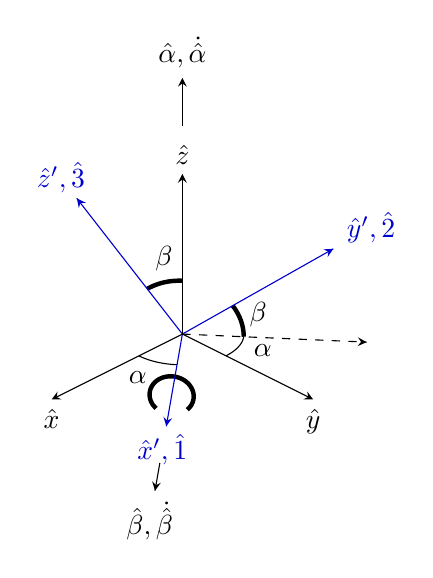
\begin{tikzpicture}
    \def\p{0.12}
    \def\q{0.667}
    \def\s{0.333}
    \def\Lx{1.2}
    \def\Ly{1.3}
    \def\Lo{1.6}
    \def\Lm{1.4}
    \def\Ln{1.7}
    \def\a{40}
    \def\b{35}
    \begin{axis}[
        scale=2.5,
        axis equal,
        axis lines=none,
        xtick=\empty,
        ytick=\empty,
        ztick=\empty,
        xmin=-\Lm,xmax=\Lm,
        ymin=-\Lm,ymax=\Lm,
        zmin=-\Lm,zmax=\Lm,
        view={135}{30},
        no markers,
        >=stealth,
        disabledatascaling,
        ]
       
        %beta vector 
        \addplot3+[black, postaction={decorate},
            decoration={markings,
                mark=at position 1.0 with {\arrow{stealth}},
            }]
            coordinates {(\Lm*cos(\a),\Lm*sin(\a),0) 
                (\Ln*cos(\a),\Ln*sin(\a),0)
            }
            node[pos=2.1] {$\hat{\beta},\dot{\hat{\beta}}$};
        %beta rotate arcs
        \addplot3+[black,ultra thick,variable=\t,
            domain=0:\b,smooth,samples=20,
            samples y=0]
            ({-\s*cos(\t)*sin(\a)},{\s*cos(\t)*cos(\a)},{\s*sin(\t)})
            node[pos=0.7,right] {$\beta$}
            ;
        \addplot3+[black, ultra thick,variable=\t,
            domain=90:90+\b,smooth,samples=20,
            samples y=0]
            ({-\s*cos(\t)*sin(\a)},{\s*cos(\t)*cos(\a)},{\s*sin(\t)})
            node[pos=0.5,above] {$\beta$}
            ;
        %beta rotate vec
        \addplot3+[black,solid,ultra thick,
            %postaction={decorate},
            %decoration={markings,
            %    mark=at position 1.0 with {\arrow{stealth}},
            %}, 
            variable=\t,
            domain=-45:225,smooth,samples=20,
            samples y=0]
            ({\q*cos(\a)-\p*cos(\t)*sin(\a)},
            {\q*sin(\a)+\p*cos(\t)*cos(\a)},{\p*sin(\t)})
            ;

        %alpha vector
        \draw [->] (axis cs:0,0,\Ly) -- (axis cs:0,0,\Lo) 
            node [above] {$\hat{\alpha},\dot{\hat{\alpha}}$};
        %alpha rotate arcs
        \addplot3+[black,solid,variable=\t,
            domain=0:\a,smooth,samples=20,
            samples y=0]
            ({\s*cos(\t)},{\s*sin(\t)},{0})
            node[pos=0.5,below left] {$\alpha$}
            ;
        \addplot3+[black,solid,variable=\t,
            domain=90:90+\a,smooth,samples=20,
            samples y=0]
            ({\s*cos(\t)},{\s*sin(\t)},{0})
            node[pos=1.1,below right] {$\alpha$}
            ;
   
        %z', 3
        \addplot3+[blue!80!black,solid,postaction={decorate},
            decoration={markings,
                mark=at position 1.0 with {\arrow{stealth}},
            }] 
            coordinates {(0,0,0) 
                ({sin(\a)*sin(\b)} ,{-cos(\a)*sin(\b)} ,{cos(\b)} )}
            node[pos=1.15] {$\hat{z}',\hat{3}$}
            ;
        %x',1,y',2
        \addplot3+[blue!80!black, solid, postaction={decorate},
            decoration={markings,
                mark=at position 1.0 with {\arrow{stealth}},
            }]
            coordinates {(0,0,0) (cos(\a),sin(\a),0)}
            node[pos=1.25] {$\hat{x}',\hat{1}$};
        \addplot3+[blue!80!black, solid, postaction={decorate},
            decoration={markings,
                mark=at position 1.0 with {\arrow{stealth}},
            }]
            coordinates {(0,0,0) 
                ({-sin(\a)*cos(\b)} , {cos(\a)*cos(\b)} , {sin(\b)} )
            } 
            node[pos=1.25] {$\hat{y}',\hat{2}$}
            ;
        \addplot3+[black, dashed, postaction={decorate},
            decoration={markings,
                mark=at position 1.0 with {\arrow{stealth}},
            }]
            coordinates {(0,0,0) (-sin(\a),cos(\a),0)} 
            %node[pos=1.25] {$\hat{y}',\hat{2}$}
            ;
 
        %Inertial coordinates
        \draw [->] (axis cs:0,0,0) -- (axis cs:1,0,0) 
            node[below] {$\hat{x}$}
            ;
        \draw [->] (axis cs:0,0,0) -- (axis cs:0,1,0)
            node[below] {$\hat{y}$}
            ;
        \draw [->] (axis cs:0,0,0) -- (axis cs:0,0,1)
            node[above] {$\hat{z}$}
            ;
    \end{axis}
\end{tikzpicture}
\end{minipage}
\begin{minipage}{0.49\textwidth}
%Rotated by gamma
\centering
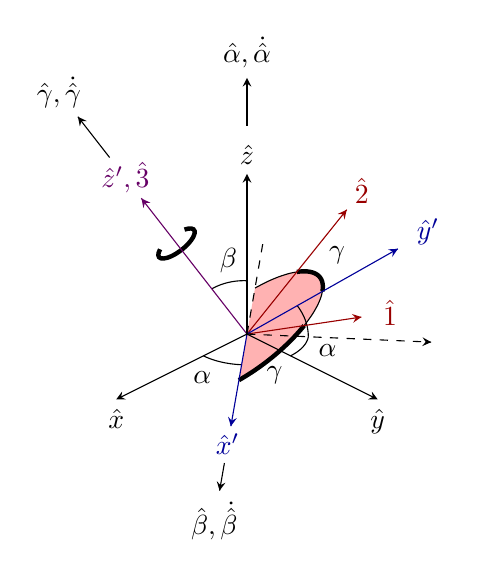
\begin{tikzpicture}
    \def\p{0.12}
    \def\h{0.5}
    \def\q{0.667}
    \def\s{0.333}
    \def\Lx{1.2}
    \def\Ly{1.3}
    \def\Lo{1.6}
    \def\Lm{1.4}
    \def\Ln{1.7}
    \def\a{40}
    \def\b{35}
    \def\g{55}
    \begin{axis}[
        scale=2.5,
        axis equal,
        axis lines=none,
        xtick=\empty,
        ytick=\empty,
        ztick=\empty,
        xmin=-\Lm,xmax=\Lm,
        ymin=-\Lm,ymax=\Lm,
        zmin=-\Lm,zmax=\Lm,
        view={135}{30},
        no markers,
        >=stealth,
        disabledatascaling,
        ]
       
        %gamma vector
        \addplot3+[black,solid,postaction={decorate},
            decoration={markings,
                mark=at position 1.0 with {\arrow{stealth}},
            }] 
            coordinates {({\Ly*sin(\a)*sin(\b)},{-\Ly*cos(\a)*sin(\b)},
                {\Ly*cos(\b)} )
                ({\Lo*sin(\a)*sin(\b)} ,{-\Lo*cos(\a)*sin(\b)} ,{\Lo*cos(\b)} )
            }
            node[pos=1.6] {$\hat{\gamma},\dot{\hat{\gamma}}$}
            ;
        %gamma rotate arc (180 deg)
        \addplot3+[black, solid, fill=red!30!white,
            variable=\t,domain=0:180,
            smooth,samples=20,samples y=0
            ]
            ({\h*cos(\a)*cos(\t)-\h*sin(\a)*cos(\b)*sin(\t)},
            {\h*sin(\a)*cos(\t)+\h*cos(\a)*cos(\b)*sin(\t)},
            {\h*sin(\b)*sin(\t)})
            ;
        \addplot3+[black, solid, ultra thick, 
            variable=\t,domain=90:90+\g,
            smooth,samples=20,samples y=0
            ]
            ({\h*cos(\a)*cos(\t)-\h*sin(\a)*cos(\b)*sin(\t)},
            {\h*sin(\a)*cos(\t)+\h*cos(\a)*cos(\b)*sin(\t)},
            {\h*sin(\b)*sin(\t)})
            node[pos=0.5,above right] {$\gamma$}
            ;
        \addplot3+[black, solid, ultra thick,
            variable=\t,domain=0:\g,
            smooth,samples=20,samples y=0
            ]
            ({\h*cos(\a)*cos(\t)-\h*sin(\a)*cos(\b)*sin(\t)},
            {\h*sin(\a)*cos(\t)+\h*cos(\a)*cos(\b)*sin(\t)},
            {\h*sin(\b)*sin(\t)})
            node[pos=0.5,below] {$\gamma$}
            ;
        %gamma rotate vec
        \addplot3+[black, solid, ultra thick,
            variable=\t,domain=-110:160,
            smooth,samples=20,samples y=0
            ]
            ({\q*sin(\a)*sin(\b)+\p*cos(\a)*cos(\t)-\p*sin(\a)*cos(\b)*sin(\t)},
            {-\q*cos(\a)*sin(\b)+\p*sin(\a)*cos(\t)+\p*cos(\a)*cos(\b)*sin(\t)},
            {\q*cos(\b)+\p*sin(\b)*sin(\t)})
            ;

        %beta vector 
        \addplot3+[black, solid, postaction={decorate},
            decoration={markings,
                mark=at position 1.0 with {\arrow{stealth}},
            }]
            coordinates {({\Lm*cos(\a)},{\Lm*sin(\a)},0) 
                (\Ln*cos(\a),\Ln*sin(\a),0)
            }
            node[pos=2.1] {$\hat{\beta},\dot{\hat{\beta}}$};
        %beta rotate arcs
        \addplot3+[black,solid,variable=\t,
            domain=0:\b,smooth,samples=20,
            samples y=0]
            ({-\s*cos(\t)*sin(\a)},{\s*cos(\t)*cos(\a)},{\s*sin(\t)})
            %node[pos=0.7,right] {$\beta$}
            ;
        \addplot3+[black,solid,variable=\t,
            domain=90:90+\b,smooth,samples=20,
            samples y=0]
            ({-\s*cos(\t)*sin(\a)},{\s*cos(\t)*cos(\a)},{\s*sin(\t)})
            node[pos=0.5,above] {$\beta$}
            ;

        %alpha vector
        \draw [->] (axis cs:0,0,\Ly ) -- (axis cs:0,0,\Lo) 
            node [above] {$\hat{\alpha},\dot{\hat{\alpha}}$};
        %alpha rotate arcs
        \addplot3+[black,solid,variable=\t,
            domain=0:\a,smooth,samples=20,
            samples y=0]
            ({\s*cos(\t)},{\s*sin(\t)},{0})
            node[pos=0.5,below left] {$\alpha$}
            ;
        \addplot3+[black,solid,variable=\t,
            domain=90:90+\a,smooth,samples=20,
            samples y=0]
            ({\s*cos(\t)},{\s*sin(\t)},{0})
            node[pos=1.1,below right] {$\alpha$}
            ;
   
        %z', 3
        \addplot3+[violet!80!black,solid,postaction={decorate},
            decoration={markings,
                mark=at position 1.0 with {\arrow{stealth}},
            }] 
            coordinates {(0,0,0) 
                ({sin(\a)*sin(\b)} ,{-cos(\a)*sin(\b)} ,{cos(\b)} )}
            node[pos=1.15] {$\hat{z}',\hat{3}$}
            ;
        %x',1,y',2
        \addplot3+[red!60!black, solid, postaction={decorate},
            decoration={markings,
                mark=at position 1.0 with {\arrow{stealth}},
            }]
            coordinates {(0,0,0) 
            ({cos(\a)*cos(\g)-sin(\a)*cos(\b)*sin(\g)},
            {sin(\a)*cos(\g)+cos(\a)*cos(\b)*sin(\g)},{sin(\b)*sin(\g)})}
            node[pos=1.25] {$\hat{1}$}
            coordinate[pos=0.5] (half1);
        \addplot3+[blue!60!black, solid, postaction={decorate},
            decoration={markings,
                mark=at position 1.0 with {\arrow{stealth}},
            }]
            coordinates {(0,0,0) (cos(\a),sin(\a),0)}
            node[pos=1.2] {$\hat{x}'$}
            coordinate[pos=0.5] (halfxp);
        \addplot3+[black, dashed]
            coordinates {(0,0,0) (-cos(\a),-sin(\a),0)}
            ;
        \addplot3+[red!60!black, solid, postaction={decorate},
            decoration={markings,
                mark=at position 1.0 with {\arrow{stealth}},
            }]
            coordinates {(0,0,0) 
                ({-cos(\a)*sin(\g)-sin(\a)*cos(\b)*cos(\g)},
                {-sin(\a)*sin(\g)+cos(\a)*cos(\b)*cos(\g)},{sin(\b)*cos(\g)})
            } 
            node[pos=1.15] {$\hat{2}$}
            coordinate[pos=0.5] (half2)
            ;
        \addplot3+[blue!60!black, solid, postaction={decorate},
            decoration={markings,
                mark=at position 1.0 with {\arrow{stealth}},
            }]
            coordinates {(0,0,0) 
                ({-sin(\a)*cos(\b)} , {cos(\a)*cos(\b)} , {sin(\b)} )
            } 
            node[pos=1.2] {$\hat{y}'$}
            coordinate[pos=0.5] (halfyp)
            ;
        \addplot3+[black, dashed, postaction={decorate},
            decoration={markings,
                mark=at position 1.0 with {\arrow{stealth}},
            }]
            coordinates {(0,0,0) (-sin(\a),cos(\a),0)} 
            %node[pos=1.25] {$\hat{y}',\hat{2}$}
            ;
        %\draw[thick,black,solid] (halfxp) -- (axis cs:0,0,0) -- (half1);
        %\draw[thick,black,solid] (halfyp) -- (axis cs:0,0,0) -- (half2);
 
        %Inertial coordinates
        \draw [->] (axis cs:0,0,0) -- (axis cs:1,0,0) 
            node[below] {$\hat{x}$}
            ;
        \draw [->] (axis cs:0,0,0) -- (axis cs:0,1,0)
            node[below] {$\hat{y}$}
            ;
        \draw [->] (axis cs:0,0,0) -- (axis cs:0,0,1)
            node[above] {$\hat{z}$}
            ;
    \end{axis}
\end{tikzpicture}
\end{minipage}
\end{center}
\end{figure}

The vector $\vec{\alpha}$ points along the 
$z$ axis, even after rotating the other angles. Second, $\vec{\beta}$ rotates 
the $z'$ and $3$ axes away from the $z$ axis, around the $x'$ axis, and 
always points along $x'$ axis even after the final rotation. Lastly, 
$\gamma$ rotates the $1$ and $2$ axes within the plane of $x'$ and $y'$. 
$z'$ and $3$ remain colinear so that $\vec{\gamma}$ points along these 
two axes. With these defined you can use the angles to relate the three 
coordinate systems and solve Euler's equations with torque. For compactness, 
I will abbreviate $\sin$ and $\cos$ of the angles as shown below.
\begin{align}
    c_\alpha &=\cos\alpha \quad c_\beta=\cos\beta \quad c_\gamma=\cos\gamma 
        \notag\\
    s_\alpha &= \sin\alpha \quad s_\beta=\sin\beta \quad s_\gamma=\sin\gamma 
        \notag\\
    \begin{bmatrix}
        \hat{x}' \\
        \hat{y}' \\
        \hat{z}'
    \end{bmatrix}
    &=
    \begin{bmatrix}
        c_\alpha & s_\alpha & 0 \\
        -s_\alpha c_\beta & c_\alpha c_\beta & s_\beta \\
        s_\alpha s_\beta & -c_\alpha s_\beta & c_\beta
    \end{bmatrix}
    \begin{bmatrix}
        \hat x \\
        \hat y \\
        \hat z
    \end{bmatrix}
    =
    \begin{bmatrix}
        c_\gamma &  -s_\gamma & 0 \\
        s_\gamma & c_\gamma & 0 \\
        0 & 0 & 1
    \end{bmatrix}
    \begin{bmatrix}
        \hat1 \\
        \hat2 \\
        \hat3
    \end{bmatrix}
    \notag\\
    \begin{bmatrix}
        \hat1 \\
        \hat2 \\
        \hat3
    \end{bmatrix}
    &=
    \begin{bmatrix}
        (c_\alpha c_\gamma - s_\alpha c_\beta s_\gamma) &
            (s_\alpha c_\gamma + c_\alpha c_\beta s_\gamma) &
            s_\beta s_\gamma \\
        -(c_\alpha s_\gamma+s_\alpha c_\beta c_\gamma) &
            -(s_\alpha s_\gamma-c_\alpha c_\beta c_\gamma) &
            s_\beta c_\gamma \\ 
        s_\alpha s_\beta & - c_\alpha s_\beta & c_\beta
    \end{bmatrix}
    \begin{bmatrix}
        \hat x\\
        \hat y\\
        \hat z
    \end{bmatrix}
    =
    \begin{bmatrix}
        c_\gamma & s_\gamma & 0 \\
        -s_\gamma & c_\gamma & 0 \\
        0 & 0 & 1
    \end{bmatrix}
    \begin{bmatrix}
        \hat{x}' \\
        \hat{y}' \\
        \hat{z}'
    \end{bmatrix}
    \notag\\
    \begin{bmatrix}
        \hat x\\
        \hat y\\
        \hat z
    \end{bmatrix}
    &=
    \begin{bmatrix}
        c_\alpha & -s_\alpha c_\beta & s_\alpha s_\beta \\
        s_\alpha & c_\alpha c_\beta & -c_\alpha s_\beta \\
        0 & s_\beta & c_\beta
    \end{bmatrix}
    \begin{bmatrix}
        \hat{x}' \\
        \hat{y}' \\
        \hat{z}'
    \end{bmatrix}
    =
    \begin{bmatrix}
        (c_\alpha c_\gamma - s_\alpha c_\beta s_\gamma) &
            -(c_\alpha s_\gamma+ s_\alpha c_\beta c_\gamma) &
            s_\alpha s_\beta \\
        (s_\alpha c_\gamma + c_\alpha c_\beta s_\gamma) &
            -(s_\alpha s_\gamma- c_\alpha c_\beta c_\gamma) &
            -c_\alpha s_\beta \\ 
        s_\beta s_\gamma & s_\beta c_\gamma & c_\beta
    \end{bmatrix}
    \begin{bmatrix}
        \hat1 \\
        \hat2 \\
        \hat3
    \end{bmatrix}
    \label{123toxyz}
\end{align}

These transformations can be acquired by looking at the projections of 
the different unit vectors onto the other frames' unit vectors, then 
making some substitutions. They can also be acquired through a composition of 
multiple rotations about the 3, then 1, then 3 axes by the different 
respective angles. I've put these transformations in the clearer matrix form, 
which also lets you see that the inverse transformation matrices are simply the 
transpose of each other, since all three coordinate systems are orthogonal.
Though I have cast it in terms of a vector of unit vectors, they can equally 
apply to the components of a vector in those coordinates. I will 
demonstrate this. Let $\overline{A}$ 
be the final matrix in Eq \ref{123toxyz} so that 
$\vec u(xyz)=\overline{A}\vec u(123)$, where $\vec u$ is the vector of unit
vectors in the coordinate system described. This relationship 
says the following is true for another vector, such as $\vec\omega$, 
which does not need to be modified for being in a rotating reference frame. 
Only its components change.
\begin{align*}
    \hat{x} &= A_{x1}\hat{1}+A_{x2}\hat{2}+A_{x3}\hat{3} \\
    \hat{y} &= A_{y1}\hat{1}+A_{y2}\hat{2}+A_{y3}\hat{3} \\
    \hat{z} &= A_{z1}\hat{1}+A_{z2}\hat{2}+A_{z3}\hat{3} \\
    \vec{\omega}&=\omega_x\hat{x}+\omega_y\hat{y}+\omega_z\hat{z} \\
    &=\omega_x\left(A_{x1}\hat{1}+A_{x2}\hat{2}+A_{x3}\hat{3} \right)
    +\omega_y\left(A_{y1}\hat{1}+A_{y2}\hat{2}+A_{y3}\hat{3}\right)
    +\omega_z\left(A_{z1}\hat{1}+A_{z2}\hat{2}+A_{z3}\hat{3}\right) \\
    &=\left(\omega_xA_{x1}+\omega_yA_{y1}+\omega_zA_{z1}\right)\hat 1
    +\left(\omega_xA_{x2}+\omega_yA_{y2}+\omega_zA_{z2}\right)\hat 2  
    +\left(\omega_xA_{x3}+\omega_yA_{y3}+\omega_zA_{z3}\right)\hat 3 \\
    &= \omega_1\hat 1 +\omega_2\hat 2 +\omega_3\hat 3 \\
    \begin{bmatrix}
        \omega_1 \\
        \omega_2 \\
        \omega_3
    \end{bmatrix}
    &=
    \begin{bmatrix}
        \omega_xA_{x1}+\omega_yA_{y1}+\omega_zA_{z1} \\
        \omega_xA_{x2}+\omega_yA_{y2}+\omega_zA_{z2} \\
        \omega_xA_{x3}+\omega_yA_{y3}+\omega_zA_{z3}
    \end{bmatrix}
    =
    \begin{bmatrix}
        A_{x1} & A_{y1} & A_{z1} \\
        A_{x2} & A_{y2} & A_{z2} \\
        A_{x3} & A_{y3} & A_{z3}
    \end{bmatrix}
    \begin{bmatrix}
        \omega_x \\
        \omega_y \\
        \omega_z
    \end{bmatrix}
    \\
    \vec{\omega}_{123} &= \overline{A}^T\vec{\omega}_{xyz} \\
    \vec{\omega}_{xyz} &= \overline{A}\vec{\omega}_{123}
\end{align*}

We need to relate these angles to the object's angular velocity and 
the angular velocity primed coordinate system. Imagine 
an infinitesimal rotation about some general direction, $d\vec\theta$. 
The angle vectors may not add to $\vec{\theta}$, but because we are using
infinitesimal vectors $(\vec{d\alpha},\vec{d\beta},\vec{d\gamma})$ will 
add to $\vec{d\theta}$. Dividing by the infinitesimal time interval, we get:
\begin{align}
    \vec\omega &= \dot{\vec{\alpha}}+\dot{\vec{\beta}}+\dot{\vec{\gamma}} \\
    \vec\omega' &= \dot{\vec{\alpha}}+\dot{\vec{\beta}}
\end{align}
$\vec\omega'$ should be interpreted as the rate of rotation of the 
$\hat{z}'$ axis and therefore the ($\hat{x}',\hat{y}',\hat{z}'$) coordinate 
system relative to the inertial one. It is not the rate of rotation 
around the $\hat{z}'$ axis, since that is clearly 
$\dot{\vec{\gamma}}$. Correspondingly, $\vec{\omega}$ is the rotation 
of the ($\hat1,\hat2,\hat3$) coordinate system relative to the 
inertial coordinate system. These will be useful for solving rotation problems.

Usually, 
an energy equation is used to find the three nutational modes (it is 
also possible there will be no nutation, with just 
precession or with a sleeping top). There may be a way to show this nutation 
using Euler's equations, 
but since they are nonlinear, it may be difficult. Also 
note that, since torque from gravity 
will always keep the $L_z$ and $L_{z'}$ components the same, nutation must 
be due to the fact that $\vec{\omega}$ doesn't point perfectly along the 
symmetry axis (which also occurs with zero torque - hence a poorly spiraled 
football) and
because $\vec{\omega}$ doesn't point along $\vec{L}$, 
since the rotation matrix would have to be proportional to 
an identity matrix, not even 
just diagonal, for $\vec{\omega}$ to be colinear with $\vec{L}$.

\subsubsection{Euler's Equations and Angles with a Gravitational Torque}

We can use the angle relationships above to find Euler's equations for a 
rotating object with cylindrical symmetry, like a bike wheel or top,
 attached at a single fixed point which is not the center 
of mass. Luckily the parallel axis theorem shows that once we start with 
a diagonal rotational inertia matrix, shifting from 
the center of mass origin to a new origin directly 
along one of the principal axes still 
yields a diagonal rotational inertia matrix. This is exactly what we want 
since the ideal example is a bike wheel or top fixed at one end, which 
has a symmetry axis (one principal axis) along the axle and, because of 
its cylindrical symmetry along that axis, we can pick any two 
perpendicular vectors as the others, see Eq \ref{isymshift}. The 
principal axes will still be aligned with the symmetry axes for the 
object in the center of mass frame. The components of the 
rotational inertia with the fixed point at the origin will use the following
variables, true for both the $(x',y',z')$ and $(1,2,3)$ reference frames
again because of the object's cylindrical symmetry:
\begin{equation*}
    \overline{I} = 
    \begin{bmatrix}
        I & 0 & 0 \\
        0 & I & 0 \\
        0 & 0 & I_s 
    \end{bmatrix}
\end{equation*}

Let's assume the object's total mass is $M$ and the axle has a length of 
$2L$ so that the center of mass is halfway along the axle.
Because the force of gravity points down, along the $\hat{z}$ axis, 
and $\hat{z}'$ and $\hat{3}$ point along the axle, the torque from 
gravity will be aligned with $\hat{x}'$ at all times:
\begin{align*}
    \vec{\tau} &= MgL\sin\beta\hat{x}' \\
        &= MgL\sin\beta(\cos\gamma\hat{1} -\sin\gamma\hat{2})
\end{align*}

Both the primed and body-fixed coordinates are noninertial so Euler's 
equations will involve the cross product with the angular velocity. Having 
already computed what this is for body-fixed coordinates, the 
$(1,2,3)$ frame's Euler's equations follow directly.
\begin{align*}
    \vec\omega &= (\dot\alpha\sin\beta\sin\gamma+\dot\beta\cos\gamma)\hat{1}
        +(\dot\alpha\sin\beta\cos\gamma-\dot\beta\sin\gamma)\hat{2} 
        +(\dot\alpha\cos\beta+\dot\gamma)\hat{3}\\
    \begin{bmatrix}
        \tau_{1} \\
        \tau_{2} \\
        \tau_{3} 
    \end{bmatrix}
    &=
    \begin{bmatrix}
        MgL\sin\beta\cos\gamma \\
       -MgL\sin\beta\sin\gamma \\
        0 
    \end{bmatrix}
    =
    \begin{bmatrix}
        I\dot{\omega}_{1} +\omega_{2}\omega_{3}(I_s-I) \\
        I\dot{\omega}_{2} +\omega_{3}\omega_{1}(I-I_s) \\
        I_s\dot{\omega}_{3}
    \end{bmatrix}
    =\\
    &
    \begin{bmatrix}
        I(\ddot\alpha\sin\beta\sin\gamma 
        + \dot\alpha\dot\beta\cos\beta\sin\gamma +
            \dot\alpha\dot\gamma\sin\beta\cos\gamma 
            + \ddot\beta\cos\gamma
            - \dot\beta\dot\gamma\sin\gamma) 
            +(\dot\alpha\sin\beta\cos\gamma-\dot\beta\sin\gamma)
            (\dot\alpha\cos\beta + \dot\gamma)(I_s-I) \\
        I(\ddot\alpha\sin\beta\cos\gamma 
            + \dot\alpha\dot\beta\cos\beta\cos\gamma 
            - \dot\alpha\dot\gamma\sin\beta\sin\gamma 
            - \ddot\beta\sin\gamma - \dot\beta\dot\gamma\cos\gamma)
            +(\dot\alpha\cos\beta+\dot\gamma)
            (\dot\alpha\sin\beta\sin\gamma+\dot\beta\cos\gamma)(I-I_s) \\
        I_s(\ddot\alpha\cos\beta-\dot\alpha\sin\beta +\ddot\gamma)
    \end{bmatrix}
\end{align*}
The latter relationships, Euler's equations in the ($1,2,3$) frame, 
are pretty hideous. The added information tracks the rotation by the 
angle $\gamma$ around the $\hat3$ axis, but the equations are 
complicated enough, as they without this information. I'll only pursue Euler's 
equations in the ($x',y',z'$) frame. 
Note that, since we aren't including any torque due to 
friction of the wheel moving around the axle, the expected 
gradual decrease in $\dot\gamma$ will not be there. 

Recall that $\vec{\omega}$ in Euler's equation (whose general form is 
repeated below) is the 
rotation of the coordinate system. It was derived using a body-fixed coordinate 
system, so that the rotation of the coordinate system told you the 
rotation of all particles in the object. Naively trying to transform Euler's 
equation in the finished form will lead to errors, since the first terms 
in Euler's equations involved $\vec{\omega}$ and the second terms 
involved both $\vec{\omega}'$ in the cross product, and $\vec{\omega}$ 
in the angular momentum. We can take advantage of how 
$\overline{I}$ is an identical diagonal matrix in both $(1,2,3)$ and 
$(x',y',z')$. The following shows what I mean and the 
correct way to do it, with all quantities in the $(x',y',z')$ basis:
\begin{align}
    \vec{\tau} &= \dot{\vec{L}} +\vec{\omega}'\times\vec{L} \notag\\
    \begin{bmatrix}
        L_{x'} \\
        L_{y'} \\
        L_{z'}
    \end{bmatrix}
    &= 
    \begin{bmatrix}
        I\omega_{x'} \\
        I\omega_{y'} \\
        I_s\omega_{z'}
    \end{bmatrix}
    \notag\\
    \begin{bmatrix}
        \tau_{x'} \\
        \tau_{y'} \\
        \tau_{z'}
    \end{bmatrix}
    &=
    \begin{bmatrix}
        I\dot{\omega}_{x'}+\omega'_{y'}\omega_{z'}I_s-\omega'_{z'}\omega_{y'}I\\
        I\dot{\omega}_{y'}+\omega'_{z'}\omega_{x'}I-\omega'_{x'}\omega_{z'}I_s\\
        I_s\dot{\omega}_{z'}+\omega'_{x'}\omega_{y'}I-\omega'_{y'}\omega_{x'}I
    \end{bmatrix}
\end{align}
The angular velocity vectors, for tracking the rotation of the 
primed coordinate system and motion of the object, itself, are:
\begin{align}
    \vec\omega' &= \dot\beta\hat{x}'+\dot\alpha\sin\beta\hat{y}'
        +\dot\alpha\cos\beta\hat{z}' \\
    \vec\omega &= \dot\beta\hat{x}'+\dot\alpha\sin\beta\hat{y}'
        +(\dot\alpha\cos\beta+\dot\gamma)\hat{z}' 
\end{align}
The angular momentum vector expanded in this basis is:
\begin{align}
    \begin{bmatrix}
        L_{x'} \\
        L_{y'} \\
        L_{z'}
    \end{bmatrix}
    &= 
    \begin{bmatrix}
        I\dot\beta \\
        I\dot\alpha\sin\beta \\
        I_s(\dot\alpha\cos\beta+\dot\gamma)
    \end{bmatrix}
    =
    \begin{bmatrix}
        I\dot\beta \\
        I\dot\alpha\sin\beta \\
        I_sS
    \end{bmatrix}
\end{align}
I defined the term $S$, as the component of the object's 
angular velocity along the primary axis, $\hat{z}'$:
\begin{equation}
    S = \omega_{z'}=\dot\alpha\cos\beta+\dot\gamma
\end{equation}
This will be useful because, as we'll see, $S$ is constant for this 
problem.

Noting that the only difference between $\vec{\omega}$ and $\vec{\omega}'$ 
is the $z'$-component, we can now 
put this together to get Euler's equations in the $(x',y',z')$ 
frame.
\begin{align}
    \begin{bmatrix}
        \tau_{x'} \\
        \tau_{y'} \\
        \tau_{z'} 
    \end{bmatrix}
    &=
    \begin{bmatrix}
        MgL\sin\beta \\
        0 \\
        0 
    \end{bmatrix}
    =
    \begin{bmatrix}
        I\dot{\omega}_{x'}+\omega'_{y'}\omega_{z'}I_s-\omega'_{z'}\omega_{y'}I\\
        I\dot{\omega}_{y'}+\omega'_{z'}\omega_{x'}I-\omega'_{x'}\omega_{z'}I_s\\
        I_s\dot{\omega}_{z'}
    \end{bmatrix}
    =
    \begin{bmatrix}
        I\ddot\beta +\dot\alpha\sin\beta SI_s 
            - \dot\alpha\cos\beta\dot\alpha\sin\beta I \\
        I(\ddot\alpha\sin\beta + \dot\alpha\dot\beta\cos\beta) 
            +\dot\alpha\dot\beta\cos\beta I
            -\dot\beta SI_s \\
        I_s\dot S 
    \end{bmatrix}
    \notag \\
    &=
    \begin{bmatrix}
        I\ddot\beta +I_sS\dot\alpha\sin\beta 
            - I\dot\alpha^2\sin\beta\cos\beta \\
        I\ddot\alpha\sin\beta + 2I\dot\alpha\dot\beta\cos\beta 
            -I_sS\dot\beta \\
        I_s\dot S 
    \end{bmatrix}
\end{align}

The third term of Euler's equation, the $z'$-component is:
\begin{align*}
    0 &= I_s\dot S = \dot{L}_{z'} \\
    I_sS &= constant
\end{align*}
This says that the component of angular momentum along the 
$\hat{z}'$-direction is constant, which is understandable since torque 
from gravity points perpendicular to $\hat{z}'$. It also points 
perpendicular to $\hat{z}$, so we should expect this angular 
momentum components is constant, too. To see if this is true, I'll 
need to transform into those coordinates and pull out the $\hat{z}$-component
 of $\vec{\omega}$ and $\vec{L}$.
\begin{align*}
    \vec\omega = &\dot\beta\hat{x}'+\dot\alpha\sin\beta\hat{y}'
        +(\dot\alpha\cos\beta+\dot\gamma)\hat{z}' \\
    = &\dot\beta(\cos\alpha\hat{x}+\sin\alpha\hat{y}) 
        +\dot\alpha\sin\beta(-\sin\alpha\cos\beta\hat{x}
        +\cos\alpha\cos\beta\hat{y} + \sin\beta\hat{z})\\
        &+(\dot\alpha\cos\beta+\dot\gamma)(\sin\alpha\sin\beta\hat{x} 
        -\cos\alpha\sin\beta\hat{y}+\cos\beta\hat{z}) \\
    = &\left(\dot\beta\cos\alpha
        -\dot\alpha\sin\beta\sin\alpha\cos\beta
        +(\dot\alpha\cos\beta+\dot\gamma)\sin\alpha\sin\beta\right)\hat{x} \\
        &+\left(\dot\beta\sin\alpha
        +\dot\alpha\sin\beta\cos\alpha\cos\beta
        -(\dot\alpha\cos\beta+\dot\gamma)\cos\alpha\sin\beta\right)\hat{y}\\
        &+\left(\dot\alpha\sin\beta\sin\beta
        +(\dot\alpha\cos\beta+\dot\gamma)\cos\beta\right)\hat{z} \\
    = &\left(\dot\beta\cos\alpha
        +\dot\gamma\sin\alpha\sin\beta\right)\hat{x} 
        +\left(\dot\beta\sin\alpha
        -\dot\gamma\cos\alpha\sin\beta\right)\hat{y}
        +\left(\dot\alpha+\dot\gamma\cos\beta\right)\hat{z} \\
    \omega_z = &\dot\alpha + \dot\gamma\cos\beta
\end{align*}

This component of angular velocity makes sense from a geometric perspective, 
just by looking at the figures showing Euler's angles. 
Since $\vec{L} = \overline{I}\vec{\omega}$, I either have to transform 
$\overline{I}$, as well, or notice the following change of basis 
relationship:
\begin{align*}
    \vec{L} &= \overline{I}\vec{\omega} \\
    \overline{P}\vec{L} &= \overline{P}\overline{I}\vec{\omega} \\
    \overline{P}\vec{L} &= 
        \overline{P}\overline{I}
        \left(\overline{P}^T\overline{P}\right)\vec{\omega} \\
    \overline{P}\vec{L} &=
        \left(\overline{P}\overline{I}\overline{P}^T\right)
        \left(\overline{P}\vec{\omega}\right)
\end{align*}
Here, $\overline{P}$ is the matrix transforming 
($x',y',z'$) into ($x,y,z$).
The approach of transforming $\overline{I}$ to the new coordinate system 
comes from the last line, but our way around this step comes from the 
second line. We can just left-multiply $\overline{I}\vec{\omega}$ by 
the change of basis matrix, which is essentially what I 
did to $\vec\omega$ to get $\omega_z$ a moment ago. Since $\overline{I}$ is 
diagonal and we only need the $L_z$-component, one might naively think 
that left-multiplying 
$\overline{I}\vec{\omega}$ by $\overline{P}$ is equivalent to just multiplying 
$\omega_z$ by $I_s$:
\begin{equation*}
    L_z = \left(\overline{P}
        \left(\overline{I}\vec{\omega}\right)\cdot\hat{z}\right) \neq 
        I_s(\dot\alpha + \dot\gamma\cos\beta)
\end{equation*}
The last relationship is not the correct form for $L_z$ 
because different terms in $\overline{I}\vec{\omega}$ simplified to make
our form for $\omega_z = \dot\alpha+\dot\gamma\cos\beta$. 
I'll compute the full form for $\vec\omega$ and $\overline{I}$ in the 
($x,y,z$) basis. Note that $\overline{P}$ is the matrix taking the 
column vector ($x',y',z'$) to ($x,y,z$) from our transformation matrices 
above, as you would intuitively expect, since our 
goal is to take vectors in the former basis to the latter basis. 
Starting from vectors and matrices in ($x',y',z'$):
\begin{align}
    \vec{L} = \overline{I}\vec{\omega} &=
    \begin{bmatrix}
        I\omega_{x'} \\
        I\omega_{y'} \\
        I_s\omega_{z'}
    \end{bmatrix}
    =
    \begin{bmatrix}
        I\dot\beta \\
        I\dot\alpha\sin\beta \\
        I_s(\dot\alpha\cos\beta+\dot\gamma)
    \end{bmatrix}
    =
    \begin{bmatrix}
        I\dot\beta \\
        I\dot\alpha\sin\beta \\
        I_sS
    \end{bmatrix}
    \notag \\
    \overline{P} &= 
    \begin{bmatrix}
        \cos\alpha & -\sin\alpha\cos\beta & \sin\alpha\sin\beta \\
        \sin\alpha & \cos\alpha\cos\beta & -\cos\alpha\sin\beta \\
        0 & \sin\beta & \cos\beta
    \end{bmatrix}
     \\
   \overline{P}\vec{L}=\overline{P}(\overline{I}\vec{\omega}) &=
    \begin{bmatrix}
        I\dot\beta\cos\alpha-I\dot\alpha\sin\beta\sin\alpha\cos\beta 
            +I_s(\dot\alpha\cos\beta+\dot\gamma)\sin\alpha\sin\beta \\
        I\dot\beta\sin\alpha+I\dot\alpha\sin\beta\cos\alpha\cos\beta
            -I_s(\dot\alpha\cos\beta+\dot\gamma)\cos\alpha\sin\beta \\
        I\dot\alpha\sin\beta\sin\beta
            +I_s(\dot\alpha\cos\beta+\dot\gamma)\cos\beta
    \end{bmatrix}
    \notag \\
    \vec{L}_{(x,y,z)}&=
    \begin{bmatrix}
        I\dot\beta\cos\alpha+(I_sS
            -I\dot\alpha\cos\beta)\sin\alpha\sin\beta \\
        I\dot\beta\sin\alpha+(I\dot\alpha\cos\beta
            -I_sS)\cos\alpha\sin\beta \\
        I\dot\alpha\sin^2\beta +I_sS\cos\beta
    \end{bmatrix}
    \\
    &=
    \begin{bmatrix}
        I\dot\beta\cos\alpha+(I_s-I)\dot\alpha\sin\alpha\sin\beta\cos\beta 
            +I_s\dot\gamma\sin\alpha\sin\beta \\
        I\dot\beta\sin\alpha+(I-I_s)\dot\alpha\cos\alpha\sin\beta\cos\beta
            -I_s\dot\gamma\cos\alpha\sin\beta \\
        \dot\alpha(I\sin^2\beta+I_s\cos^2\beta)+I_s\dot\gamma\cos\beta
    \end{bmatrix}
    \\
    \vec{\omega}_{(x,y,z)}&=
    \begin{bmatrix}
        \dot\beta\cos\alpha +\dot\gamma\sin\alpha\sin\beta \\
        \dot\beta\sin\alpha-\dot\gamma\cos\alpha\sin\beta \\
        \dot\alpha+\dot\gamma\cos\beta
    \end{bmatrix}
\end{align}
The result in the second to last line is $\vec{L}$ in the ($x,y,z$) basis.
The last line is $\vec{\omega}$ in the ($x,y,z$) basis, which I included 
for easy future comparison. For sake of completeness, I will calculate 
$\overline{I}$ in the ($x,y,z$) basis:
\begin{align}
    \overline{P}\overline{I}\overline{P}^T &=
    \begin{bmatrix}
        \cos\alpha & -\sin\alpha\cos\beta & \sin\alpha\sin\beta \\
        \sin\alpha & \cos\alpha\cos\beta & -\cos\alpha\sin\beta \\
        0 & \sin\beta & \cos\beta
    \end{bmatrix}
    \begin{bmatrix}
        I & 0 & 0 \\
        0 & I & 0 \\
        0 & 0 & I_s
    \end{bmatrix}
    \begin{bmatrix}
        \cos\alpha & \sin\alpha & 0 \\
        -\sin\alpha\cos\beta & \cos\alpha\cos\beta & \sin\beta \\
        \sin\alpha\sin\beta & -\cos\alpha\sin\beta & \cos\beta
    \end{bmatrix}
    \notag\\
    &=
    \begin{bmatrix}
        \cos\alpha & -\sin\alpha\cos\beta & \sin\alpha\sin\beta \\
        \sin\alpha & \cos\alpha\cos\beta & -\cos\alpha\sin\beta \\
        0 & \sin\beta & \cos\beta
    \end{bmatrix}
    \begin{bmatrix}
        I\cos\alpha & I\sin\alpha & 0 \\
        -I\sin\alpha\cos\beta & I\cos\alpha\cos\beta & I\sin\beta \\
        I_s\sin\alpha\sin\beta & -I_s\cos\alpha\sin\beta & I_s\cos\beta
    \end{bmatrix}
    \notag \\
    \overline{I}_{(x,y,z)}&=
    \begin{bmatrix}
        I\cos^2\alpha + \sin^2\alpha(I\cos^2\beta +I_s\sin^2\beta)
            & \sin\alpha\cos\alpha(I-I\cos^2\beta-I_s\sin^2\beta)
            & (I_s-I)\sin\alpha\sin\beta\cos\beta \\
        \sin\alpha\cos\alpha(I - I\cos^2\beta - I_s\sin^2\beta)
            & I\sin^2\alpha+\cos^2\alpha(I\cos^2\beta+I_s\sin^2\beta)
            & (I-I_s)\cos\alpha\sin\beta\cos\beta \\
        (I_s-I)\sin\alpha\sin\beta\cos\beta 
            & (I-I_s)\cos\alpha\sin\beta\cos\beta
            & I\sin^2\beta+I_s\cos^2\beta
    \end{bmatrix}
\end{align}
Notice that $\overline{I}_{(x,y,z)}$ is still symmetric, as it should be. Our 
primary goal in doing this transformation was to see if 
the $z$-component of $\vec{L}$ is constant with Euler's equations 
for our rotating bike wheel under gravity scenario. This component and 
its derivative are:
\begin{align*}
    L_z &=\dot\alpha(I\sin^2\beta+I_s\cos^2\beta)+I_s\dot\gamma\cos\beta 
        =I\dot\alpha\sin^2\beta+I_s\dot\alpha\cos^2\beta
        +I_s\dot\gamma\cos\beta \\
    \dot{L}_z &=
        I\ddot\alpha\sin^2\beta+2I\dot\alpha\dot\beta\sin\beta\cos\beta
        +I_s\ddot\alpha\cos^2\beta-2I_s\dot\alpha\dot\beta\sin\beta\cos\beta
        +I_s\ddot\gamma\cos\beta -I_s\dot\beta\dot\gamma\sin\beta
\end{align*}
Written in terms of the spin, $S$, these become:
\begin{align}
     L_z &=I\dot\alpha\sin^2\beta +I_sS\cos\beta \\
     \dot{L}_z&=I\ddot\alpha\sin^2\beta+2I\dot\alpha\dot\beta\sin\beta\cos\beta 
            + I_s\dot S\cos\beta - I_sS\dot\beta\sin\beta \notag\\
        &=I\ddot\alpha\sin^2\beta+2I\dot\alpha\dot\beta\sin\beta\cos\beta 
            - I_sS\dot\beta\sin\beta
\end{align}
The very last line follows from what we previously determined, that
the angular momentum $z'$-component is constant, which means $\dot S=0$.
Let's compare this to the $y'$-component of Euler's equation:
\begin{align*}
    \tau_{y'} = 0 &= 
        I\ddot\alpha\sin\beta + 2I\dot\alpha\dot\beta\cos\beta 
            -I_sS\dot\beta \\
    0\sin\beta= 0 &=
        I\ddot\alpha\sin^2\beta + 2I\dot\alpha\dot\beta\sin\beta\cos\beta 
            -I_sS\dot\beta\sin\beta = \dot{L}_z
\end{align*}
The $z$-component of angular momentum is, indeed, constant.

Looking back at $\vec{L}_{(x',y',z')}$ and $\vec{\omega}_{(x',y',z')}$, 
notice that they must point in different directions, due to $I$ and $I_s$
being different values. The angle between these 
two vector quantities, along with the angles 
between $\vec{\omega}$ and $\hat{z}'$ and between $\vec{L}$ and $\hat{z}'$
turn out to be quite hideous. The most useful way to approach this 
is with conservation of energy, but that is not what I wish this 
document to be about. The relevant sections of Analytical Mechanics by 
Fowles and Cassiday, 6th ed. include include section 9.8 and the previous 
sections to establish their notation.

I can assume an initial condition for the angular velocity and 
momentum. If the bike wheel is started at some nonzero angle 
$\beta_o$ from the $z$-axis, with initial conditions:
\begin{align*}
    \dot\alpha_o &=0 \\
    \dot\beta_o&=0 \\
    \dot\gamma_o &> 0 \\
    \Rightarrow S &= \dot\alpha\cos\beta + \dot\gamma = \dot\gamma_o
\end{align*}
Since $S$ was determined in our general analysis to be constant, then 
it will always remain this value, which is why I did not give it a subscript 
specifying this as its initial state. Euler's equations become:
\begin{align}
    \begin{bmatrix}
        MgL\sin\beta \\
        0 \\
        0 
    \end{bmatrix}
    &=
    \begin{bmatrix}
        I\ddot\beta +I_sS\dot\alpha\sin\beta 
            - I\dot\alpha^2\sin\beta\cos\beta \\
        I\ddot\alpha\sin\beta + 2I\dot\alpha\dot\beta\cos\beta 
            -I_sS\dot\beta \\
        I_s\dot S 
    \end{bmatrix}
    =
    \begin{bmatrix}
        I\ddot\beta +(I_s-I)\dot\alpha^2\sin\beta\cos\beta 
            +I_s\dot\alpha\dot\gamma\sin\beta \\
        I\ddot\alpha\sin\beta + (2I-I_s)\dot\alpha\dot\beta\cos\beta 
            -I_s\dot\beta\dot\gamma \\
        I_s\dot S 
    \end{bmatrix} \notag\\
    \begin{bmatrix}
        MgL\sin\beta_o \\
        0 \\
        0 
    \end{bmatrix}_{t=0}
    &=
    \begin{bmatrix}
        I\ddot\beta \\
        I\ddot\alpha\sin\beta \\
        I_s\dot S 
    \end{bmatrix}_{t=0}
\end{align}
This seems to say that, the first moment the wheel is released from 
rest, the axle drops slightly ($\beta$ accelerates in the positive 
direction). The initial angular velocity and angular momentum are:
\begin{align*}
    \begin{bmatrix}
        \omega_{x'} \\
        \omega_{y'} \\
        \omega_{z'}
    \end{bmatrix}
    &=
    \begin{bmatrix}
        \dot\beta \\
        \dot\alpha\sin\beta \\
        \dot\alpha\cos\beta + \dot\gamma
    \end{bmatrix}
    =
    \begin{bmatrix}
        \dot\beta \\
        \dot\alpha\sin\beta \\
        S
    \end{bmatrix}
    \\
    \begin{bmatrix}
        \omega_{x'} \\
        \omega_{y'} \\
        \omega_{z'}
    \end{bmatrix}_{t=0}
    &=
    \begin{bmatrix}
        0 \\
        0 \\
        \dot\gamma_o
    \end{bmatrix}_{t=0}
    =
    \begin{bmatrix}
        0 \\
        0 \\
        S
    \end{bmatrix}_{t=0}
    \\
    \begin{bmatrix}
        L_{x'} \\
        L_{y'} \\
        L_{z'}
    \end{bmatrix}
    &=
    \begin{bmatrix}
        I\omega_{x'} \\
        I\omega_{y'} \\
        I_s\omega_{z'}
    \end{bmatrix}
    =
    \begin{bmatrix}
        I\dot\beta \\
        I\dot\alpha\sin\beta \\
        I_s(\dot\alpha\cos\beta+\dot\gamma)
    \end{bmatrix}
    =
    \begin{bmatrix}
        I\dot\beta \\
        I\dot\alpha\sin\beta \\
        I_sS
    \end{bmatrix}
    \\
    \begin{bmatrix}
        L_{x'} \\
        L_{y'} \\
        L_{z'}
    \end{bmatrix}_{t=0}
    &=
    \begin{bmatrix}
        0 \\
        0 \\
        I_s\dot\gamma_o
    \end{bmatrix}_{t=0}
    =
    \begin{bmatrix}
        0 \\
        0 \\
        I_sS
    \end{bmatrix}_{t=0}
\end{align*}
Both vectors are fully aligned with the $\hat{z}'$ axis in the initial state. 
Let's look a moment later:
\begin{align*}
    \begin{bmatrix}
        MgL\sin\beta \\
        0 \\
        0 
    \end{bmatrix}_{t=\epsilon}
    &=
    \begin{bmatrix}
        I\ddot\beta \\
        I\ddot\alpha\sin\beta - I_sS\dot\beta\\
        I_s\dot S 
    \end{bmatrix}_{t=\epsilon}
    \\
    \begin{bmatrix}
        \omega_{x'} \\
        \omega_{y'} \\
        \omega_{z'}
    \end{bmatrix}_{t=\epsilon}
    &=
    \begin{bmatrix}
        \dot\beta \\
        0 \\
        \dot\gamma
    \end{bmatrix}_{t=\epsilon}
    =
    \begin{bmatrix}
        \dot\beta \\
        0 \\
        S
    \end{bmatrix}_{t=\epsilon}
    \\
    \begin{bmatrix}
        L_{x'} \\
        L_{y'} \\
        L_{z'}
    \end{bmatrix}_{t=\epsilon}
    &=
    \begin{bmatrix}
        I\dot\beta \\
        0 \\
        I_s\dot\gamma
    \end{bmatrix}_{t=\epsilon}
    =
    \begin{bmatrix}
        I\dot\beta \\
        0 \\
        I_sS
    \end{bmatrix}_{t=\epsilon}
\end{align*}
$\beta$ continues to increase, as does $\dot\beta$. 
Now also, $\alpha$ begins to acquire some positive velocity, because its value 
for acceleration is positive: 
\begin{equation*}
    \ddot{\alpha} = \frac{I_sS\dot\beta}{I\sin\beta}
\end{equation*}
The angular velocity and angular momentum are no longer 
aligned with the $\hat{z}'$ axis. Both have some component in the 
positive $\hat{x}'$ direction, at this instant. Which one points farther 
from the $\hat{z}'$ direction depends on whether $I$ is less than or greater 
than $I_s$. We'll see later that, for approximate values involved in a 
bike wheel demonstration, $\vec{L}$ always points farther from the $\hat{z}'$ 
axis than does $\vec\omega$.

Another moment later we have:
\begin{align*}
    \begin{bmatrix}
        MgL\sin\beta \\
        0 \\
        0 
    \end{bmatrix}_{t=2\epsilon}
    &=
    \begin{bmatrix}
        I\ddot\beta +I_sS\dot\alpha\sin\beta 
            - I\dot\alpha^2\sin\beta\cos\beta \\
        I\ddot\alpha\sin\beta + 2I\dot\alpha\dot\beta\cos\beta 
            -I_sS\dot\beta \\
        I_s\dot S 
    \end{bmatrix}_{t=2\epsilon}
    =
    \begin{bmatrix}
        I\ddot\beta +(I_s-I)\dot\alpha^2\sin\beta\cos\beta 
            +I_s\dot\alpha\dot\gamma\sin\beta \\
        I\ddot\alpha\sin\beta + (2I-I_s)\dot\alpha\dot\beta\cos\beta 
            -I_s\dot\beta\dot\gamma \\
        I_s\dot S 
    \end{bmatrix}_{t=2\epsilon}
    \\
    \begin{bmatrix}
        \omega_{x'} \\
        \omega_{y'} \\
        \omega_{z'}
    \end{bmatrix}_{t=2\epsilon}
    &=
    \begin{bmatrix}
        \dot\beta \\
        \dot\alpha\sin\beta \\
        \dot\alpha\cos\beta+\dot\gamma
    \end{bmatrix}_{t=2\epsilon}
    =
    \begin{bmatrix}
        \dot\beta \\
        \dot\alpha\sin\beta \\
        S
    \end{bmatrix}_{t=2\epsilon}
    \\
    \begin{bmatrix}
        L_{x'} \\
        L_{y'} \\
        L_{z'}
    \end{bmatrix}_{t=2\epsilon}
    &=
    \begin{bmatrix}
        I\dot\beta \\
        I\dot\alpha\sin\beta \\
        I_s(\dot\alpha\cos\beta+\dot\gamma)
    \end{bmatrix}_{t=2\epsilon}
    =
    \begin{bmatrix}
        I\dot\beta \\
        I\dot\alpha\sin\beta \\
        I_sS
    \end{bmatrix}_{t=2\epsilon}
\end{align*}
Now we have the full Euler's equation for our scenario. Recognizing 
that $\dot\alpha>0$, $\dot\beta>0$, and $\beta>0$, the 
bike wheel's axis of symmetry will begin to move 
in a more complicated pattern. The angular 
velocity and momentum both have components in both the $\hat{x}'$ and 
$\hat{y}'$ directions. Since we know the $z'$-component of angular momentum is 
constant throughout this process, it may end up precessing around the 
$\hat{z}'$ axis, or not. It is not clear from these equations. We 
can find the angle that the 
angular velocity and angular momentum vectors make from the $\hat{x}'$ axis:
\begin{align}
    \frac{\omega_{y'}}{\omega_{x'}} &= \tan\Theta_{\omega,x'} = 
        \frac{\dot\alpha\sin\beta}{\dot\beta} \notag \\
    \frac{L_{y'}}{L_{x'}} &= \tan\Theta_{L,x'} =
        \frac{I\dot\alpha\sin\beta}{I\dot\beta} = 
        \frac{\dot\alpha\sin\beta}{\dot\beta} \label{xangles}
\end{align}
This is true for this problem, in general, not at 
specific times. The two vectors make the same 
angle from $\hat{x}'$, meaning that the extra vector deviation
from the $\hat{z}'$, is always colinear for $\vec{\omega}$ and $\vec{L}$. 
This vector deviation and $\hat{z}'$ form a plane that contains the 
bike wheel's axis of symmetry, the angular velocity, and the 
angular momentum vectors. 

Since $\dot\alpha$, $\beta$, and $\dot\beta$ can 
and often do change, this angle will change. Again, 
whether these vectors precess around the $\hat{z}'$ axis
 is not obvious. If $\dot\alpha$ and $\dot\beta$ oscillate and 
with the same frequency, as appears to happen with nutation, then it is 
possible that the angle made from the $\hat{x}'$ axis is constant 
if they also oscillate with the same phase. In order 
for the vector to precess around the $\hat{z}'$ symmetry axis, 
it seems the tangent of this angle would go to infinity, and indeed it would 
if the term were oscillating and $\dot\beta$ was going to zero. However, 
I should point out that because the $\hat{z}'$ axis is itself oscillating,
$\vec\omega$ making a constant angle with the $\hat{x}'$ is not a 
sort of passive oscillation of $\vec\omega$ around the $\hat{z}'$ axis 
because $\omega_{x'}$ would change sign if this was to happen.

In one phase in nutational motion, it seems $\dot\alpha$ is roughly 
constant and $\dot\beta$ is oscillating. Another 
mode appears to have the two out of phase, possibly by 90 degrees. Yet 
another appears they may be in phase, but $\dot\alpha$ may actually 
have half the frequency of $\dot\beta$. This means, in all these 
nutational modes, it seems that the $\vec\omega$ and $\vec{L}$ vectors 
do precess around the $\hat{z}'$ symmetry axis.

If $\dot\alpha$ is constant and $\dot\beta$ is 
very small or zero, as with non-nutating precession, then Equations 
\ref{xangles} approache infinity meaning that the angle from the $\hat{x}'$ 
axis approaches 90 degrees. This is positive if $\dot\alpha$ is positive and 
would mean the angular velocity and angular momentum vectors are 
pointing in the $\hat{z}$ direction, upward, and not precessing around 
the $\hat{z}'$ symmetry axis.

We can look at the deviation 
of the angular velocity and angular momentum vectors from the $\hat{z}'$ axis 
by recognizing that the $x'$ and $y'$ components of each 
vector can add to a single vector perpendicular to $\hat{z}'$, and the 
angle that $\vec{\omega}$ and $\vec{L}$ make from the $\hat{z}'$ axis 
are given by:
\begin{align}
    \tan\Theta_{\omega,z'} &= 
        \frac{|\vec{\omega}_{x'}+\vec{\omega}_{y'}|}{\omega_{z'}} = 
        \frac{\sqrt{\dot\alpha^2\sin^2\beta+\dot\beta^2}}{S} 
        \notag \\
    \tan\Theta_{L,z'} &= 
        \frac{|\vec{L}_{x'}+\vec{L}_{y'}|}{L_{z'}} = 
        \frac{I}{I_s}\frac{\sqrt{\dot\alpha^2\sin^2\beta+\dot\beta^2}}{S} 
        \notag \\
    \frac{\tan\Theta_{L,z'}}{\tan\Theta_{\omega,z'}} &=\frac{I}{I_s} 
        \label{zangles}
\end{align}
Again, this is true for this problem, in general, not just for a 
specific time. It is clear that the individual angles do change as 
$\dot\alpha$, $\beta$, and $\dot\beta$ change, but the ratio of these 
angles is always constant for this rigid body. We will see that 
for a typical bike wheel demonstration, the angular momentum points 
farther from the $\hat{z}'$ axis, the axis of symmetry, than the 
angular velocity does. Notice also that, 
since $S$ is constant but $\dot\alpha>0$ and $\beta>0$, then $\dot\gamma$ 
must have decreased slightly, since:
\begin{equation*}
    \dot\gamma = S - \dot\alpha\cos\beta
\end{equation*}

I will stray away from forces and torques momentarily. 
Though it is not obvious, this makes some sense
from an energy perspective, because the kinetic energy was entirely 
due to rotation around the axis, initially. However, as the entire 
bike wheel gains kinetic energy from rotating in the $\hat{\alpha}$ and 
$\hat{\beta}$ directions, those particles that were not 
moving before are now, and this kinetic energy has to come from somewhere.
It could come from the very slight drop in height of those particles, 
and therefore, a drop in gravitational potential energy. A more thorough 
analysis of the energy, using work due to the force of gravity, 
should reveal more insight but I will not pursue this here.

At this point, it seems the future motion of $\alpha$, and $\beta$ depend 
more carefully on the particular values of $I$, $I_s$, and $\beta$. 
Some light could be shed on this by approximating a real bike wheel to see 
which moment of inertia term is greater. Recall the entire 
bike wheel apparatus has mass $M$ and length $2L$ with a center of 
mass at $L$ from the origin. If the wheel part is 
approximated as a thin, uniform disk with radius $R$, a small
thickness $d$, and mass $m\lesssim M$, and the axle which does not 
spin with the wheel has length $2L\approx2R$, mass $\mu\ll m\lesssim M$, and 
very small radius $\rho$, then we could either calculate or just look 
up the values for the rotational inertia terms for each part of the 
bike wheel. Recall that, since the rotational inertia involes 
a sum or integral, the total rotational inertia is the sum of the component 
rotational inertia terms.
\begin{align*}
    \overline{I}_{cm} &= \overline{I}_{wheel,cm} + \overline{I}_{axle,cm} \\
    \overline{I}_{wheel,cm} &=
    \begin{bmatrix}
        \frac{m}{12}(3R^2+d^2) & 0 & 0 \\
        0 & \frac{m}{12}(3R^2+d^2) & 0 \\
        0 & 0 & \frac{m}{2}R^2
    \end{bmatrix}
    \approx
    \begin{bmatrix}
        \frac{m}{4}R^2 & 0 & 0 \\
        0 & \frac{m}{4}R^2 & 0 \\
        0 & 0 & \frac{m}{2}R^2
    \end{bmatrix}
    \\
    \overline{I}_{axle,cm} &=
    \begin{bmatrix}
        \frac{\mu}{12}(3\rho^2+4L^2) & 0 & 0 \\
        0 & \frac{\mu}{12}(3\rho^2+4L^2) & 0 \\
        0 & 0 & 0
    \end{bmatrix}
    \approx
    \begin{bmatrix}
        \frac{\mu}{3}L^2 & 0 & 0 \\
        0 & \frac{\mu}{3}L^2 & 0 \\
        0 & 0 & 0
    \end{bmatrix}
    \\
    \overline{I}_{cm} &\approx
    \begin{bmatrix}
        \frac{m}{4}R^2+\frac{\mu}{3}L^2 & 0 & 0 \\
        0 & \frac{m}{4}R^2+\frac{\mu}{3}L^2 & 0 \\
        0 & 0 & \frac{m}{2}R^2
    \end{bmatrix}
    \approx
    \begin{bmatrix}
        \frac{M}{4}R^2 & 0 & 0 \\
        0 & \frac{M}{4}R^2 & 0 \\
        0 & 0 & \frac{M}{2}R^2
    \end{bmatrix}
    \\
    \overline{I} &=
    \begin{bmatrix}
        I & 0 & 0 \\
        0 & I & 0 \\
        0 & 0 & I_s
    \end{bmatrix}
    \approx
    \begin{bmatrix}
        \frac{M}{4}R^2+ML^2 & 0 & 0 \\
        0 & \frac{M}{4}R^2+ML^2  & 0 \\
        0 & 0 & \frac{M}{2}R^2
    \end{bmatrix}
    \\
    I &\approx \frac{M}{4}R^2+ML^2 \approx \frac{5M}{4}R^2 \\
    I_s &\approx \frac{M}{2}R^2 \approx \frac{2}{5}I
\end{align*}
So for typical bike wheels for a demonstration like this, $I$ is 
significantly greater than $I_s$, due to having to rotate 
the entire apparatus about its endpoint. This result supports 
the point that for a typical bike wheel precessing about the 
end point, the angle that the angular momentum makes from the $\hat{z}'$ 
axis, the axis of symmetry, is greater than that made by the angular velocity, 
though they always lie in the same plane containing themselves 
and the $\hat{z}'$ axis. Specifically, we found previously that:
\begin{equation*}
    \frac{\tan\Theta_{L,z'}}{\tan\Theta_{\omega,z'}} = \frac{I}{I_s}
        \approx\frac{5}{2}
\end{equation*}
These angles depend on $\dot\alpha$, $\beta$, and $\dot\beta$, as shown 
in Equations \ref{zangles}.

What we know so far is consistent with the notion that the bike wheel 
will precess in the positive $\hat{\alpha}$ direction, which matches 
simpler scenario of a bike wheel at $\beta=90^\circ=\pi/2$. We saw from 
Equation \ref{xangles} that when this happens, the angular velocity and 
angular momentum vectors point vertically up (if $\dot\alpha>0$).
I know from energy considerations in other sources
that giving the bike wheel a sharp push forward and backward 
($\dot\alpha >0, \dot\alpha<0$, respectively) can yield two different 
nutational modes. Another mode occurs when $\dot\alpha=0$ initially, 
when the bike wheel has the correct spin, and angle $\beta$. 
During nutation in general, we saw from Equations 
\ref{xangles} that $\vec\omega$ and $\vec L$ can wobble in 
more complicated but interesting ways, as the $\dot\alpha$ and $\dot\beta$ 
angles oscillate. This includes precession of $\vec\omega$ and $\vec L$
around the $\hat{z}'$ symmetry axis. While this occurs, the fixed 
components of angular momentum ($L_{z'}$ and $L_z$) 
will not oscillate, despite the oscillation of 
the symmetry axis of the bike wheel, and the angular velocity.

I could pursue this further to find $\alpha$, $\beta$, and 
$\gamma$ with time. Some insight can be made by using the graph method for 
analyzing nonlinear differential equations, defining the rates of change of 
each Euler angle's velocity so it becomes a system of four equations and four 
variables, but each equation is only a first order autonomous differential 
equation. Then one could identify the stable points by setting the 
various rates to zero, perhaps linearizing, and looking at different 
regimes. This yields a slight bit of insight like the condition for 
stable precession when $\dot\beta=0$ and $\ddot\alpha=0$, 
but the real interesting behavior appears outside of these stable point 
regimes, during nutation. Instead, I prefer to refer 
the reader, to the relevant sections of Analytical Mechanics by 
Fowles and Cassiday, 6th ed. include include section 9.8 and the previous 
sections to establish their notation, or another analytical mechanics book.

Computer simulation would be a better tool for analyzing this rotational 
motion further. This is greatly helped by modifying 
Euler's equations for quaternions. It significantly simplifies 
problems for computation and clarity, with no down sides that I know of. See 
the introduction to quaternions with an applciation to rigid body dynamics. 
A particular  unit-length quaternion can be used for rotation and 
its conditions are very simple which one can find with 5 minutes of 
Googling. There are relationships between quaternion 
multiplication (which is noncommutative, like matrix multiplication) and 
vector dot and cross products. Quaternion use for rotation has the 
benefits of being more numerically stable, less computationally 
expensive (because you need to compute fewer terms), is immune to 
gimbal lock which occurs with matrix multiplication, and finally its 
representation of rotation around some generic vector in three dimensions by 
a certain angle is much simpler than rotation matrices, which 
require either a change of basis to align the rotation axes with a generic 
vector or a hideous single $3\times3$ matrix. 

\subsection{Quaternion use for Euler's Equations Simulation}

Quaternions were invented by William Rowan Hamilton in 1843 as a generalization 
of complex numbers. Where $i=\sqrt{-1}$ and $i^2=-1$, and a complex number 
can be made of a real and imaginary part: $a + bi$, a quaternion has 
three different imaginary-like parts: $a+bi+cj+dk$. These imaginary numbers 
obey the following multiplication rules:
\begin{align}
    ijk&=-1, \\
    i^2=j^2&=k^2=-1.
\end{align}
From these, you can derive the following multiplication table and you 
discover that quaternions are non-commutative, as this multiplication 
table is neither symmetric nor anti-symmetric:
\begin{center}
    $
    \begin{tabular}[h!]{c || c | c | c | c}
         & 1 & i & j & k \\
        \hline
        \hline
        1 & 1 & i & j & k \\
        \hline
        i & i & -1 & k & -j \\
        \hline
        j & j & -k & -1 & i \\
        \hline
        k & k & j & -i & -1 
    \end{tabular}
    $
\end{center}
While quaternion multiplication is not commutative, it is associative. 

There is a simpler way to represent quaternions and quaternion multiplication:
\begin{align}
    q &= (a, \vec b) \\
    q_1q_2 &= (a_1a_2-\vec b_1\cdot\vec b_2,a_1\vec b_2+a_2\vec b_1
        +\vec b_1\times\vec b_2 )
\end{align}
Quaternions can have a conjugate and inverse like so:
\begin{align}
    q^c &= (a,-\vec b) \\
    q^{-1} &= \frac{(a,-\vec b)}{qq^c}
\end{align}
The denominator can be thought of as the norm of a quaternion because 
the result is always real and the result is consistent with the idea of the
norm of a scalar and a vector, the quaternion's constituents:
\begin{equation}
    qq^c = q^cq = (a^2 + |b|^2,0) = a^2 + |b|^2
\end{equation}
This means if you want to normalize a quaternion, you can apply the following:
\begin{equation}
    q' = \frac{q}{\sqrt{qq^c}}
\end{equation}

A particular unit-length quaternion can be used for rotation, 
as can the product of multiple similar quaternions. If an object rotates by 
$\theta$ around a unit-vector $\hat n$, the rotation quaternion would be:
\begin{equation}
    q = (\cos(\theta/2),\sin(\theta/2)\hat n)
\end{equation}
The inverse of this rotation quaternion undoes the rotation:
\begin{equation*}
    q^{-1} = q^c = (\cos(\theta/2),-\sin(\theta/2)\hat n)
\end{equation*}
It would be applied to another vector $\vec{x}$ made into a 
pure-imaginary quaternion like so:
\begin{equation}
    q(0,\vec{x})q^{-1} \label{qrotate}
\end{equation}
The resultant imaginary part gives the rotated vector. Multiple rotations 
around different axes and with different angles, 
can be composed into a single quaternion, with the first rotation on the right.
The Euler equations are simplest to solve in the 123-coordinate system, but 
to visualize, we need to convert it to the $xyz$ system. To solve 
the Euler equations numerically, and do so while avoiding gimbal lock which 
happens when axes overlap and a degree of freedom is lost, I need 
to maintain the quaternion to rotate/transform the angular velocity components 
in the 123 system back to the $xyz$ system. 

Recall my particular 
Euler angles come from a 3-1-3 sequence. The transformation matrix from 
Eq \ref{123toxyz} is equivalent to taking a product of rotations, 
in the 123 basis, by $-\gamma$ about the 3 axis, then $-\beta$ about the 
1 axis, then $-\alpha$ about the 3 axis. Because these are orthogonal matrices
and the transpose is the inverse, a negative transpose of a rotation 
matrix about a simple axis is the same as the original. 
This inspired the idea of taking the product of rotation quaternions, 
from right to left, by the positive angles: $\gamma$, $\beta$, $\alpha$. 
For simplicity, I will adopt similar abbreviations as Eq \ref{123toxyz}.
\begin{align}
    c_a &=\cos(\alpha/2)\quad c_b=\cos(\beta/2)\quad c_g=\cos(\gamma/2)\notag\\
    s_a &=\sin(\alpha/2)\quad s_b=\sin(\beta/2)\quad s_g=\sin(\gamma/2)\notag\\
    q &= (c_a,0,0,s_a)(c_b,s_b,0,0)(c_g,0,0,s_g) \\
     &= 
    \begin{bmatrix}
        (c_ac_g - s_as_g)c_b \\
        (c_ac_g + s_as_g)s_b \\
        (s_ac_g - c_as_g)s_b \\
        (s_ac_g + c_as_g)c_b
    \end{bmatrix} \label{q123toxyz}    
\end{align}
Notice how symmetric this quaternion's form is, compared to the 
transformation matrices of Eq \ref{123toxyz}. 

To update the quaternion after 
a change in angle of $\vec d\theta_{123}=\vec{\omega}_{123}dt$, 
right multiply this quaternion by:
\begin{equation}
    dq = (\cos(d\theta/2),\sin(d\theta/2)d\hat{\theta})
\end{equation}
Note that this is equivalent to left-multiplying by the quaternion in the 
$xyz$-coordinate system. It makes sense that we need to right-multiply by 
this $dq$ to construct a quaternion that will 
take vectors in the 123 frame to the $xyz$ frame. The quaternion in Eq 
\ref{q123toxyz} is a composite of rotations from right to left, in the 
opposite order in which they occured. This $dq$ is the last rotation to 
occur so it must be the first to be undone when applied to vectors 
for converting bases. The $\vec{\omega}$ vector in the 
$xyz$-coordinate system is acquired by applying $q$ from Eq \ref{q123toxyz}
in the manner prescribed by Eq \ref{qrotate}. You do the same thing 
to rotate the vectors defining the orientation of your object.

The last thing to note is how to get the 3-1-3 Euler angles from the 
quaternion in Eq \ref{q123toxyz}. With the quaternion as written, 
the following relationship gives the set of angles. Use the $\text{atan2}$ 
function as described below 
to allow for the full domain for each angle. This relationship uses 
the form $q=(q_0,q_1,q_2,q_3)$ and note that if you take 
$q_2\rightarrow-q_2$, this switches $\alpha$ and $\gamma$:
\begin{align}
    \alpha &=\text{atan2}\left\{2(q_1q_3+q_0q_2),2(q_0q_1-q_2q_3)\right\}
        \notag \\
    \beta &= \text{acos}\left\{(q_3^2 - q_2^2)+(q_0^2-q_1^2)\right\} \notag \\
    \gamma &= \text{atan2}\left\{2(q_1q_3-q_0q_2),2(q_0q_1+q_2q_3)\right\}
\end{align}
The products of 2 in the $\text{atan2}$ functions are superfluous, since 
they cancel, and can therefore be left out, but they demonstrate the use of 
the double angle formulas for verifying these relationships. Otherwise, 
terms have been associated for better numerical stability. I have 
implemented these quaternion methods in two simulations of rotational motion at 
www.glowscript.org/\#/user/owendix/.

\section{Appendix} 
\subsection{Reference for the Basics}\label{apx:ref}

\begin{itemize}
    \item All position, velocity, and acceleration values, as well as 
    all quantities derived from them, assume some inertial
    coordinate system has been chosen. An inertial coordinate system is one 
    where objects moving without external forces move with a constant velocity.
    \item Vectors are written like $\vec{a}$, while scalars, including the 
    magnitudes of  vectors, are written like $a$.
    \item Dot notation is used to mean the full time derivative of a quantity, 
    which is distributive over addition and constant factors can be 
    effectively factored out of a derivative, because the derivative of the 
    factor is zero when expanded with the product rule (here $m$ is constant):
    \begin{equation*}
        \frac{d}{dt}(\vec{a}+m\vec{b}) = \dot{\vec{a}}+\frac{d}{dt}(m\vec{b}) 
        = \dot{\vec{a}}+\dot{m}\vec{b} + m\dot{\vec{b}} 
        = \dot{\vec{a}}+m\dot{\vec{b}}
    \end{equation*}
    \item The position vector of some object is $\vec{r}$
    \item The object's velocity, $\vec{v} = d\vec{r}/dt$ is written as 
    $\dot{\vec{r}}$
    \item The object's acceleration is 
    $\vec{a} = d\vec{v}/dt=d^2\vec{r}/dt^2=\ddot{\vec{r}}$
    \item The momentum of an object is $\vec{p}=m\vec{v}=m\dot{\vec{r}}$
    \item The angular momentum of an object is $\vec{L}=\vec{r}\times\vec{p}$,
    where $\times$ indicates the vector cross product. 
    \item The cross product $\vec{a}=\vec{b}\times\vec{c}$ yields a vector 
    $\vec{a}$ perpendicular to the plane of $\vec{b}$ and $\vec{c}$ 
    in a right-handed sense (which is only a plane if they are not colinear) 
    and having magnitude $a=bc\sin\alpha$, where $\alpha$ is the angle 
    between the vectors $\vec{b}$ and $\vec{c}$, found by translating them so 
    their tails are placed at the same point. Note if $\vec{b}$ and $\vec{c}$
    are colinear then $\alpha=0$ or $\pi$ and $a=0$. The components of 
    $\vec{a} = (a_x,a_y,a_z)$ can be calculated with a $3\times3$ determinant
    with rows equal to $(\hat{x},\hat{y},\hat{z})$, $\vec{b}$, and $\vec{c}$, 
    respectively. This yields:
    \begin{equation} \label{cross}
        \vec{a}=(a_x,a_y,a_z) = (b_yc_z - b_zc_y, b_zc_x - b_xc_z, 
        b_xc_y-b_yc_x)
    \end{equation}
    \item You can verify from the above expression that scalar multiplication
    of vectors can be factored out of a cross product, so
    $(m\vec{a})\times\vec{b} = \vec{a}\times(m\vec{b}) = m(\vec{a}\times{b})$.
    Cross products are also distributive over addition of vectors
    $\vec{a}\times(\vec{b}+\vec{c})=\vec{a}\times\vec{b}+\vec{a}\times\vec{c}$, 
    and 
    $(\vec{a}+\vec{b})\times\vec{c}=\vec{a}\times\vec{c}+\vec{b}\times\vec{c}$
    and are anti-commutative so
    $\vec{b}\times\vec{c} = - \vec{c}\times\vec{b}$. The distributive
    property means that, 
    if a vector is not explicitly dependent on the index of a summation, 
    its cross product with other vectors can be pulled out of the sum.
    \item The torque due to some force $\vec{F}$ that acts on a particle 
    at point $\vec{r}$ (relative to the origin of the coordinate system)
    is written as $\vec{\tau}=\vec{r}\times\vec{F}$.
    \item The center of mass of an object, 
    which is a weighted average of the how the mass of the object is 
    distributed, with particles $k=1,2,\ldots,K$ and total mass
    $M=\sum_{k=1}^K m_k$ is given by:
    \begin{equation} \label{rcm}
        \vec{r}_{cm} = \frac{\sum_{k=1}^K m_k\vec{r}_k}{M}
    \end{equation}
    \item You can get two somewhat obvious but significant ideas by shifting
    the position vector $\vec{r}_i$, relative to some generic origin 
    so a new one has its origin at 
    the center of mass, itself: $\vec{r}_i = \vec{r}_{cm}+\vec{r}_{i\,cm}$. 
    Read $\vec{r}_{i\,cm}$ as the position of the 
    $i$-th particle relative to the center of mass. Substituting this:
    \begin{align}
        \vec{r}_{cm} &= \frac{\sum_{k=1}^K m_k(\vec{r}_{cm}+\vec{r}_{k\,cm})}{M}
            = \frac{\sum_{k=1}^K m_k\vec{r}_{cm}
            + \sum_{k=1}^K m_k\vec{r}_{k\,cm}}{M} = 
            \vec{r}_{cm} + \frac{\sum_{k=1}^K m_k\vec{r}_{k\,cm}}{M} \notag \\
        \vec{r}_{cm} &= \vec{r}_{cm} + \vec{r}_{cm\,cm} \notag \\
        0 & = \vec{r}_{cm\, cm} = \frac{\sum_{k=1}^K m_k\vec{r}_{k\,cm}}{M} 
            \label{rcmcm}\\
        0 & = \dot{\vec{r}}_{cm\,cm} = M\dot{\vec{r}}_{cm\,cm} = 
            \vec{p}_{cm\,cm} = \sum_{k=1}^K m_k\dot{\vec{r}}_{k\,cm}
            \label{pcmcm}
    \end{align}

    $\vec{r}_{cm\,cm}$ should be read as the position of the 
    center of mass, relative to the center of mass. 
    The second to last line means that with the center of mass at the 
    origin of the system, the center of mass of the system is at the origin 
    (obviously). The first step in the 
    last line of equations follows by taking the time 
    derivative of all sides. This means that the velocity of the 
    center of mass, relative to the center of mass is zero, and therefore, 
    the total momentum of the system, relative to the center of mass, 
    (and its rate of change) are zero too. 
    These ideas are significant, and will come up later. 
    
\end{itemize}

\subsection{NonInertial Reference Frames}

An inertial coordinate system is one where Newton's 1st law holds: 
where objects move in a straight line, as measured by that coordinate system.
A noninertial coordinate system is one where this does not hold. If the 
origin of a coordinate system is accelerating through space, 
it is easy to see, that 
measurements of a particle under no external forces, will not match that for 
a particle moving in a straight line with a constant speed. Also if the 
basis vectors of a coordinate system are rotating, even with a constant 
speed and orientation, the measured position for a particle will not match 
that for a straight line, either. What will happen, precisely?

Any vector, $\vec{A}$, exists independent of its coordinate system 
but measurements of its direction and size need to be relative to something, 
and a coordinate system serves that purpose. The vector $\vec{A}$ can be 
expanded in terms of its degree of overlap with each basis vector in the 
coordinate system:

\begin{equation}
    \vec{A} = \sum_\mu A_\mu \hat{e}_\mu = \sum_\mu A'_\mu\hat{e}'_\mu
\end{equation}

Here the two sets of unit-length,
basis vectors for the different primed and unprimed 
coordinate systems are given by $\hat{e}_\mu$ and $\hat{e}'_\mu$, respectively,
and $\mu$ runs over the different coordinate bases. 
The degree of overlap of $\vec{A}$ with each coordinate system is given 
by the following, $A_\mu = \vec{A}\cdot\hat{e}_\mu$ and 
$A'_\mu = \vec{A}\cdot\hat{e}'_\mu$. In 
the language of differential geometry, 
the basis vectors (not unit length) for a coordinate system 
are given by differentials of different coordinates 
and partial derivatives with respect to coordinates (for 
contravariant and covariant vectors), and the dot product is computed 
using the metric. The basis vectors are like a directional derivative of your 
space with respect to each coordinate.
I'll be using the simpler, less generalized unit vectors 
and the dot product will be computed in flat space (the metric is the identity
tensor). 

The differential geometric way does give us a quick way to find the 
unit vectors for a change of basis with a 
system of spatial coordinates: take the derivative with respect to the 
new coordinates of the position vector (written in terms of the new 
coordinates), then normalize. Here's an example of a change of basis from 
2-dimensional cartesian coordinates 
$\{\hat{e}_x,\hat{e}_y\}=\{\hat{x},\hat{y}\}$ 
to 2-dimensional polar coordinates 
$\{\hat{e}_r,\hat{e}_\theta\}=\{\hat{r},\hat{\theta}\}$
(cylindrical coordinates in 3-dimensions but setting $z=0$). 
\begin{align}
    \vec{r} &= x\hat{x} + y\hat{y} \notag\\
    \vec{r} &= r\cos\theta\hat{x} + r\sin\theta\hat{y} \notag\\
    \hat{e}_r = \left|\frac{\partial \vec{r}}{\partial r}\right|^{-1} 
        \frac{\partial \vec{r}}{\partial r} &= \cos\theta\hat{x} + 
        \sin\theta\hat{y} \\
    \hat{e}_\theta = \left|\frac{\partial \vec{r}}{\partial\theta}\right|^{-1} 
        \frac{\partial \vec{r}}{\partial\theta} &= -\sin\theta\hat{x} + 
        \cos\theta\hat{y} 
\end{align}

Let's consider the unprimed coordinate to be constant, fixed in space, 
and the primed coordinate system to generally be varying (though I won't 
assume how just yet).
\begin{align}
    \frac{d\vec{A}}{dt} = \dot{\vec{A}} &= \sum_\mu \dot{A}_\mu\hat{e}_\mu \\
    \dot{\vec{A}} &= \sum_\mu \dot{A}'_\mu\hat{e}'_\mu + 
        A'_\mu\dot{\hat{e}}'_\mu 
\end{align}

In the previous example, the cartesian coordinates may be the unprimed 
system, fixed 
in space, and the polar coordinates, since their direction depends on their 
location in space, could be the primed coordinates. This is not the only way 
to have variable coordinates; we could define coordinates as being fixed to 
a body as it moves and rotates through space. The first term in the 
second line, for the primed system, is in correspondence 
to the unprimed system. The second term is clearly the difference.
To know how the primed system's basis vectors change with time, 
we need to compare them to another coordinate system. It turns out most 
productive to expand this term in the primed basis vectors, since 
we ultimately want a relation between one side of an equation with 
one basis and the other side with the other basis.
\begin{equation}
    \dot{\hat{e}}'_\mu = \sum_\nu 
        \left(\dot{\hat{e}}'_\mu\cdot\hat{e}'_\nu\right)\hat{e}'_\nu
\end{equation}
The term in parentheses is an antisymmetric tensor, it switches sign when 
$\mu$ and $\nu$ are exchanged, which can be seen by 
the following given that $\hat{e}'_\mu\cdot\hat{e}'_\nu = \delta'_{\mu\nu}$:
\begin{align*}
    0 = \frac{d}{dt}\left(\hat{e}'_\mu\cdot\hat{e}'_\nu\right) &= 
        \dot{\hat{e}}'_\mu\cdot\hat{e}'_\nu + 
        \hat{e}'_\mu\cdot\dot{\hat{e}}'_\nu \\
    \dot{\hat{e}}'_\mu\cdot\hat{e}'_\nu &= -\hat{e}'_\mu\cdot\dot{\hat{e}}'_\nu
\end{align*}

Now, regardless of whether the primed system is rotating or translating or 
both, the dot product between two vectors requires they be associated with the 
same point. 
This means that no translation of the two coordinate systems 
can affect this dot product, whether that translation is inertial or not. 
In flat space, vectors can be parallel transported without changing 
the direction of the vector and in a way that is independent of the path taken 
to transport the vector. In curved space, this may pose a problem, but we 
are working in flat space, here. 
If you define:
\begin{align}
    \left(\dot{\hat{e}}'_\mu\cdot\hat{e}'_\nu\right) 
        &= \sum_\sigma\epsilon_{\mu\nu\sigma}\dot{\Omega}'_\sigma \\
    \omega_\sigma &= \dot{\Omega}'_\sigma \notag\\
    A'_\mu\dot{\hat{e}}'_\mu &= A'_\mu\sum_\nu\sum_\sigma\epsilon_{\mu\nu\sigma}
        \omega_\sigma\hat{e}'_\nu\notag\\
    \dot{\vec{A}} = \sum_\mu \dot{A}'_\mu\hat{e}'_\mu + 
        A'_\mu\dot{\hat{e}}'_\mu &= \sum_\mu \dot{A}'_\mu\hat{e}'_\mu + 
           \sum_\mu A'_\mu\sum_\nu\sum_\sigma\epsilon_{\mu\nu\sigma}
            \omega_\sigma\hat{e}'_\nu
\end{align}
The second line, defining the angular velocity, can be seen by noting that, 
if rotation is all that affects the 
dot product of the change in the prime basis vectors with the basis vector 
itself, and these unit vectors do not change length, then rotation is 
all that will affect it. Defining the angular velocity proportional to 
their degree of rotation with this levi-cevita symbol is perfectly natural.

Let's explicitly right out the different components of the second term in 
$\dot{\vec{A}}$, where the only nonzero terms come from $\mu\neq\nu\neq\sigma$:
\begin{align*}
    A'_1(\epsilon_{123}\omega_3\hat{e}'_2 + \epsilon_{132}\omega_2\hat{e}'_3) 
        & = A'_1(\omega_3\hat{e}'_2 - \omega_2\hat{e}'_3) \\
    A'_2(\epsilon_{231}\omega_1\hat{e}'_3 + \epsilon_{213}\omega_3\hat{e}'_1) 
        & = A'_2(\omega_1\hat{e}'_3 - \omega_3\hat{e}'_1) \\
    A'_3(\epsilon_{312}\omega_2\hat{e}'_1 + \epsilon_{321}\omega_1\hat{e}'_2) 
        & = A'_3(\omega_2\hat{e}'_1 - \omega_1\hat{e}'_2) 
\end{align*}

The vector is actually the sum of these and we wish to see the components 
that line up with the $\{\hat{e}'_j\}$ basis vectors, so lets add and combine 
these:

\begin{align}
    \sum_\mu A'_\mu\dot{\hat{e}}'_\mu &= 
        (\omega_2 A'_3 - \omega_3 A'_2)\hat{e}'_1 + 
        (\omega_3 A'_1 - \omega_1 A'_3)\hat{e}'_2 + 
        (\omega_1 A'_2 - \omega_2 A'_1)\hat{e}'_3 \notag\\
    &= \vec{\omega}\times\vec{A}' \notag\\
    \dot{\vec{A}} &= \dot{\vec{A}}' + \vec{\omega}\times\vec{A}
\end{align}

The $\vec{A}$ in the cross product term can be represented in any coordinate 
system, as I will soon argue. 
This is true for any vector, comparing its change in an inertial or 
noninertial (primed) coordinate system. The primed coordinate system 
could be translating or rotating and the angular velocity may change with 
time. Note the angular velocity does not have a prime because, since it is 
the rotation of the primed coordinate system itself and 
not the rotation of something within it, 
it is represented in both coordinate systems the same. The following 
supports that:

\begin{equation}
    \dot{\vec{\omega}} = \dot{\vec{\omega}}' + \vec{\omega}\times\vec{\omega} =
        \dot{\vec{\omega}}'
\end{equation}

The cross product of $\vec{\omega}$ with itself will always be zero. 
Recall a vector is independent of its coordinate representation, just what 
numbers you have aligned with each basis depends on the coordinate choice. This 
means that the cross product term can be computed in either coordinate system, 
because the two vectors and the result are independent of coordinates. Only 
the time derivative needs to be computed in the primed basis. Of course, 
when you add the two terms together, you need a common basis.

It had bothered me, previously, that when adding angular momenta of the 
orbit and spin of an object, they could simply be added directly. In a fixed 
coordinate system, perhaps it shouldn't have, but the rotations are about 
different points. This result may help alleviate some of that unease but 
I think it doesn't really relate. The real help may be that, since we can 
mentally consider only part of the system, say the spinning part, its angular 
momenta will be conserved (in that it can only change from an angular impulse 
from a net torque acting for a period of time) and the same is true if we 
mentally expand our system to include all parts. Then again, perhaps it 
does help. I'll know when I apply these results to conservation of angular 
momentum.

Let's apply this to a position vector to see how velocity and acceleration 
change a changing coordinate basis. Then I'll shift
I'll use primes to represent quantities that use the noninertial system.
\begin{align}
    \dot{\vec{r}} &= \dot{\vec{r}}^{\,\prime} 
        + \vec{\omega}\times\vec{r} \notag\\
    \dot{\vec{r}} 
        &= \left(\frac{d}{dt}\middle|_\prime + \vec{\omega}\times\right)\vec{r}
\end{align}

Again, the $\vec{\omega}$ cross product can be computed in 
either coordinate system, but just convert the result to the 
primed system afterward to be able to add this vector to the other 
term. The second line writes the equation like a linear operator. 
Applying two operators:
\begin{align}
    \ddot{\vec{r}}
        &= \left(\frac{d}{dt}\middle|_\prime + \vec{\omega}\times\right)
        \left(\frac{d}{dt}\middle|_\prime + \vec{\omega}\times\right)\vec{r} 
        \notag\\
    \ddot{\vec{r}} 
        &= \ddot{\vec{r}}^{\,\prime} + \dot{\vec{\omega}}\times\vec{r} + 
        2\vec{\omega}\times\dot{\vec{r}}^{\,\prime} + 
        \vec{\omega}\times(\vec{\omega}\times\vec{r})
\end{align}

Now let's shift the vector, showing a translating origin. This could not 
be done for a general vector because the units of the length-shift do not 
match the units of the other vector. Angular momentum has already been done 
in the main section, for the center of mass frame with the result that 
fictitious torques do not appear from translation to the center of mass-origin.
I'll use the shift $\vec{\rho}=\vec{R}+\vec{r}$ so that $\vec{\rho}$ is the 
position of the particle in an inertial frame, $\vec{R}$ is the 
position of the noninertial frame, relative to the inertial frame, and 
$\vec{r}$ is the position of the particle in the noninertial frame, making 
it the only noninertial position vector. This vector $\vec{r}$
 will be expanded using the noninertial relationships derived above.
\begin{align}
    \dot{\vec{\rho}} &= \dot{\vec{R}} + \dot{\vec{r}}^{\,\prime}
        +\vec{\omega}\times\vec{r} \notag\\
    \ddot{\vec{\rho}} 
        &= \ddot{\vec{R}} + \ddot{\vec{r}}^{\,\prime} +
        \dot{\vec{\omega}}\times\vec{r} + 
        2\vec{\omega}\times\dot{\vec{r}}^{\,\prime} + 
        \vec{\omega}\times(\vec{\omega}\times\vec{r})
\end{align}

We can find the fictitious forces by multiplying the second 
line by the total mass of the system, $M$:

\begin{align}
    M\ddot{\vec{\rho}} 
        &= M\ddot{\vec{R}} + M\ddot{\vec{r}}^{\,\prime} +
        M\dot{\vec{\omega}}\times\vec{r} + 
        2M\vec{\omega}\times\dot{\vec{r}}^{\,\prime} + 
        M\vec{\omega}\times(\vec{\omega}\times\vec{r}) \\
    &M\dot{\vec{\omega}}\times\vec{r} \tag{transverse ``force''} \\
    &2M\vec{\omega}\times\dot{\vec{r}}^{\,\prime} \tag{coriolis ``force''} \\
    &M\vec{\omega}\times(\vec{\omega}\times\vec{r}) \tag{centrifugal ``force''}
\end{align}


\subsection{Motion in a Circle}\label{apx:motioncircle}

\begin{figure}[H]
\begin{center}
\begin{tikzpicture}[scale=2]
    \draw [thick,->] (-1.5,0) -- (1.5,0) node[below]{$x$};
    \draw [thick,->] (0,-1.5) -- (0,1.5) node[right]{$y$};
    %\draw [thin,dashed,->] (-2,2) -- (-0.5,0.5) node[midway,above]{$v$};
    \draw [thin] (+0.4,0) arc (0:30:0.4); 
    \draw (0,0) circle (1);
    \draw [->] (0,0) -- (0.866025,0.5) node[midway,above]{$\vec{r}$};
    \draw (0.5,0.15) node {$\theta$};
    \draw [->] (0.866025,0.5) -- (1.2990375,.75) node [right]{$\hat{r}$};
    \draw [->] (0.866025,0.5) -- (0.616025,.9330125) node [above]{$\hat{s}$};
    %\node at (0,0) [label={below:(overhead view)}] {};
\end{tikzpicture}
\end{center}
\end{figure}

Refer to the picture above and 
start from the equation for arclength, with angle $\theta$ measured 
in radians (defining the radians), then take the derivative of both sides, 
assuming the particle is confined to a perfect circle:
\begin{align}
    \ell &= r\theta \\
    \vec{v} &= r\omega\hat{s}
\end{align}

Taking another derivative, with constant $r$, we get:
\begin{align}
    \vec{a} &= r\dot{\omega}\hat{s} + r\omega\dot{\hat{s}} \notag\\
    &= r\alpha\hat{s} + r\omega\dot{\hat{s}}
\end{align}

The first term contains the magnitude of the angular acceleration. The second 
term is nonzero because the tangent vector $\hat{s}$ does change with 
time as the particle rotates. The change in $\hat{s}$ must be 
perpendicular to $\hat{s}$ because its length does not change, visually 
you can see that $\hat{s}$ will point in the negative $\hat{r}$ direction 
as $\theta$ increases. More explicitly, though, we can expand $\hat{s}$ and 
$\hat{r}$ in terms of the fixed $\hat{x}$ and $\hat{y}$, then take 
the derivative of $\hat{s}$:
\begin{align*}
    \hat{r} &= \cos\theta\hat{x} + \sin\theta\hat{y} \\
    \hat{s} &= -\sin\theta\hat{x} + \cos\theta\hat{y} \\
    \dot{\hat{s}} &= -\omega\cos\theta\hat{x} - \omega\sin\theta\hat{y} \\
    &= -\omega(\cos\theta\hat{x} + \sin\theta\hat{y}) \\
    &= -\omega\hat{r}
\end{align*}

We end up with,
\begin{equation}
    \vec{a} = r\alpha\hat{s} - \omega^2r\hat{r} = r\alpha\hat{s} - 
        \frac{v^2}{r}\hat{r}
\end{equation}

We can do this a bit more rigorously, since we want rotational motion 
vectors to have direction and magnitude.
If we define the vector $\vec{\theta}$ as out of the plane, it would 
be convenient because it would use a constant direction characterizing the 
plane of rotation, which actually helps relate to quaternion rotation, nicely. 
Doing this:
\begin{equation}
    \hat{\theta} = \hat{r}\times\hat{s} = \hat{\omega}
\end{equation}
where the final equality follows because the particle is confined to 
a fixed circle. Note what we did previously, setting the derivative 
of the angular speed to get the angular acceleration, is still valid since 
the direction of angular velocity does not change for motion in a fixed 
circle. 

We can substitute for $\hat{s} = \hat{\omega}\times\hat{r}$, 
because:
\begin{equation}
    \hat{\omega}\times\hat{r} = (\hat{r}\times\hat{s})\times\hat{r} = 
        - \hat{r}\times(\hat{r}\times\hat{s}) = \hat{s}(\hat{r}\cdot\hat{r}) 
        - \hat{r}(\hat{r}\cdot\hat{s}) = \hat{s}
\end{equation}
Then the velocity of any particle moving in a circle will be given by the 
following, with $\vec{r}$ relative to the center of the circle:
\begin{align}
    \vec{v} &= \vec{\omega}\times\vec{r} \label{vomegar} \\
    &= r\omega\hat{s}
\end{align}

A derivative of the Eq \ref{vomegar} 
will yield the acceleration of a particle moving 
in a circle, with $\vec{r}$ relative to the center:
\begin{align}
    \vec{a} & = \dot{\vec{\omega}}\times\vec{r} + 
        \vec{\omega}\times\dot{\vec{r}} \notag\\
    &= \dot{\vec{\omega}}\times\vec{r} + 
        \vec{\omega}\times(\vec{\omega}\times\vec{r}) \notag\\
    &= \vec{\alpha}\times\vec{r} + 
        \vec{\omega}\times(\vec{\omega}\times\vec{r}) \label{aalphar} \\
    &= \alpha r\hat{s} - \omega^2 r\hat{r}
\end{align}
This is consistent with our previous attempt using magnitudes.

Note that Eq \ref{vomegar} and Eq \ref{aalphar}
are consistent with the results of explicitly relating an inertial 
and noninertial coordinate system, as it should be. 
Here, polar coordinates can be considered fixed to the 
particle as it moves through space, then the angular velocity of the 
particle is the angular velocity of the coordinate system since its orientation
changes keeping $\hat{r}$ always pointed away from the origin of the 
cartesian coordinate system.
I'll use primes to represent quantities that use the polar, noninertial system.
\begin{align}
    \dot{\vec{r}} &= \dot{\vec{r}}^{\,\prime} 
        + \vec{\omega}\times\vec{r}  \notag\\
        &= \left(\frac{d}{dt}\middle|_\prime + \vec{\omega}\times\right)\vec{r}
\end{align}
The result of the 
cross product with $\vec{\omega}$ is independent of coordinate choice, 
since the $\vec{\omega}$ and the vector are both 
independent of coordinate choice.
Applying two operators:

\begin{align}
    \ddot{\vec{r}}
        &= \left(\frac{d}{dt}\middle|_\prime + \vec{\omega}\times\right)
        \left(\frac{d}{dt}\middle|_\prime + \vec{\omega}\times\right)\vec{r} 
        \notag\\
    &= \ddot{\vec{r}}^{\,\prime} + \dot{\vec{\omega}}\times\vec{r} + 
        2\vec{\omega}\times\dot{\vec{r}}^{\,\prime} + 
        \vec{\omega}\times(\vec{\omega}\times\vec{r})
\end{align}

The vector $\vec{r}$ pointing from the origin 
of the fixed frame to the particle does not change in the polar coordinate 
system. It always points along $\hat{r}$ and has constant length. So,
\begin{align}
    \vec{v}&=\dot{\vec{r}} = \vec{\omega}\times\vec{r} \\
    \vec{a}&=\dot{\vec{\omega}}\times\vec{r} + 
        \vec{\omega}\times(\vec{\omega}\times\vec{r}) \notag\\
        &= \vec{\alpha}\times\vec{r} + 
        \vec{\omega}\times(\vec{\omega}\times\vec{r})
\end{align}

Which is, again, consistent with previous results.

\subsection{The Spiral from a Rotating Sprinkler in Space}

Imagine a sprinkler at the origin of a coordinate system rotates in the 
positive angular velocity direction at a constant speed, $\Omega_o = 2\pi/T$, 
where $T$ is its period of rotation. As it rotates, it fires 
water (or any particle, really) radially outward 
at a constant rate so that these 
particles leave the origin at the same constant speed
$v_o$ for all ejected particles. The pattern of water made 
should be some sort of spiral; let's compare to two different possible spirals.

An archimedian spiral in polar coordinates and then 
cartesian coordinates, respectively, has the equations:
\begin{align}
    r &= a + b\theta \\
    x & = r\cos\theta = (a + b\theta)\cos\theta \\
    y & = r\sin\theta = (a + b\theta)\sin\theta
\end{align}

\begin{figure}[H]
\begin{center}
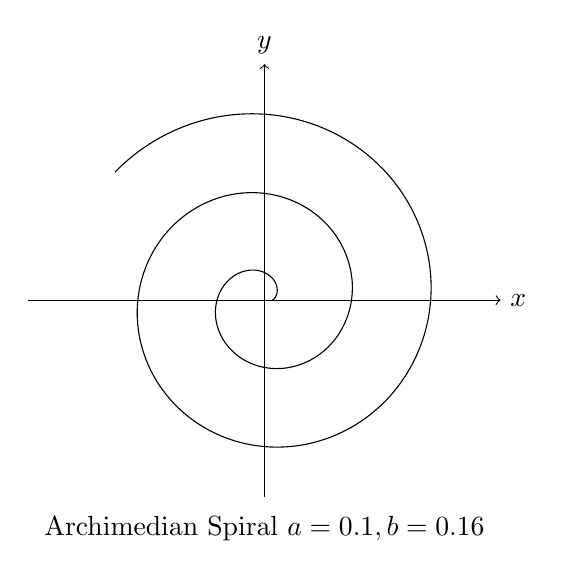
\begin{tikzpicture}
    \draw [domain=0:15,variable=\t,smooth,samples=500]
        plot ({\t r}: {0.1+0.16*\t});
    \draw [->] (-3,0) -- (3,0) node[right] {$x$};
    \draw [->] (0,-2.5) -- (0,3) node[above] {$y$};
    \node at (0,-2.5) [label={below:Archimedian Spiral $a=0.1,b=0.16$}] {};
\end{tikzpicture}
\end{center}
\end{figure}
This is the most general spiral where each branch is equally spaced with 
the next closer or farther branch at the same $\theta$.

A logarithmic spiral has the equations:
\begin{align}
    r &=a e^{b\theta} \\
    x &= a e^{b\theta}\cos\theta \\
    y &= a e^{b\theta}\sin\theta
\end{align}

\begin{figure}[H]
\begin{center}
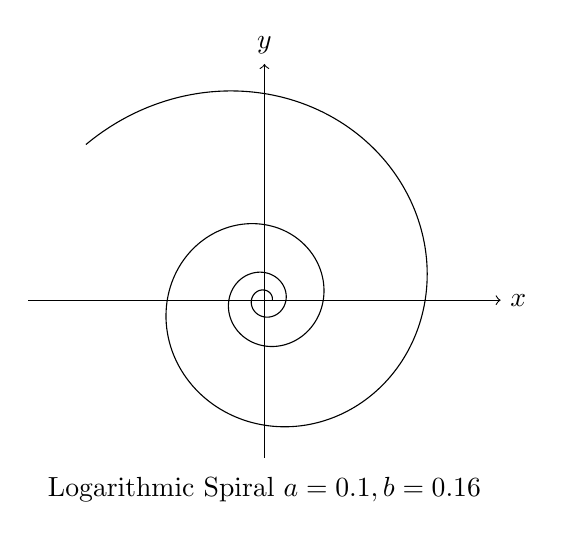
\begin{tikzpicture}
    \draw [domain=0:21.28,variable=\t,smooth,samples=500]
        plot ({\t r}: {0.1*exp(0.16*\t)});
    \draw [->] (-3,0) -- (3,0) node[right] {$x$};
    \draw [->] (0,-2) -- (0,3) node[above] {$y$};
    \node at (0,-2) [label={below:Logarithmic Spiral $a=0.1,b=0.16$}] {};
\end{tikzpicture}
\end{center}
\end{figure}
This spiral has the feature that the radial change with $\theta$ at a given 
point $(r,\theta)$ is proportional the value of $r$ at that point.

For our scenario, the radial distance from the origin will depend on 
the speed and time from when it was ejected, call it $t_e = t_e(\theta)$ 
which can be depend on the angle within the spiral we are looking at.
\begin{equation}
    r = v_o[t - t_e]
\end{equation}

I really want $r$ to be a function of $\theta$ only, so I need to find 
$t_e(\theta)$. If the sprinkler starts ($t=0$) at $\theta=0$, then 
$t_e$ is given by:
\begin{equation}
    t_e(\theta) = \theta/\Omega_o
\end{equation} 

This makes the radial distance:
\begin{equation}
    r = v_o[t - \theta/\Omega_o]
\end{equation}
Now, when we view a spiral of sprinkler, we are seeing a series of snapshots
with fixed $t$. So consider $t$ to be some fixed parameter, and we can 
analyze the shape of this spiral at this fixed time. This makes 
the equation above that for an archimedian spiral (in polar coordinates), 
with parameters $a = v_ot$ and $b = -v_o\Omega_o$. The negative sign in $b$
affects the direction of rotation of the spiral snapshot.

Compare the shape of an archimedian spiral generated by ejecting mass at a 
constant speed from an object rotating at a constant rotation rate to 
the Spiral over Norway (2009) which has several youtube videos. 


\begin{figure}[H]
\begin{center}
    \includegraphics[scale=1.4948454]{spiralNorway2009.png}
    \includegraphics{spiralNorway2009_2.png}
\end{center}
\end{figure}


The 
middle of the spiral is difficult to make out with how thick the spiral 
lines are, as you look farther from the center, it appears to match 
much closer to an archimedian spiral than a logarithmic one, since 
the spiral lines separate at a pretty constant spacing, the key signature 
of an archimedian spiral. The spiral appears to be rotating clockwise, 
making $b$ a positive number. We can estimate the $\Omega_o$ at roughly
1 revolution every 2-3 seconds or $\Omega_o\approx2.5 rad/s$, but not 
the $v_o$ for the rate that matter leaves the rocket. This would depend 
on properties of the leak, like the hole size, the pressure 
in the tank, etc. which we cannot know.

It is not clear whether the fuel is ignited. 
Other evidence points to a rocket, spinning and ejecting fuel 
at a roughly constant rate, being a good explanation. There is a 
Wikipedia entry for this event. At the end, the blackness 
expands because the fuel stream stops and is not replenished 
by the previously constant stream.

\begin{figure}[H]
\begin{center}
    \includegraphics[scale=1.581522]{spiralNorway2009_3.png}
    \includegraphics[scale=1.5]{spiralNorway2009_4.png}
\end{center}
\end{figure}

Two factors may affect the accuracy of our assumptions of a rotating 
source of matter. We assumed constant rotation and that the matter 
traveled outward at a constant rate. The two factors in question, 
to the degree that they matter - which is possibly quite slight, seem to 
cancel so that an apparently archimedian spiral should still 
fit the shape of this exhaust. The rocket loses mass as it spins 
which would tend to increase its angular velocity with time, however 
if the mass is not lost very fast this will be minimal. This perhaps slight 
increase in its rotation rate with time would tend to condense the spirals 
closer to the rocket compared to those that are formed by matter released 
a little while earlier, making it appear a bit more logarithmic. Again, 
if this is a slow enough loss compared to its rotational inertia which it 
quite possibly is, it 
may not be visible over a time scale of the life of the matter in the spiral 
at any given time. The other factor is that the matter being ejected won't expand outward at a constant velocity, exactly, since there is atmosphere in the 
way and gravity pulling it down. However, just like how air in a room is 
relatively homogeneous over those length scales, and roughly behaves the 
ideal gas law (meaning interactions are minimal), this would have a minimal 
effect. It would condense the entire spiral and if the ejected matter was 
actually brought to a rough halt, may make the outer part of the spiral seem to 
condense the most. Air resistance on small particles like gas is roughly 
linear with velocity, not quadratic like for larger objects, 
so its effects would not be seen the most at the inside of the spiral. Again, 
though, these two effects seem to be quite small. So we should still expect an 
archimedian spiral. For a demonstration of this, see my simulations at 
www.glowscript.org/\#/user/owendix/.

\end{document}
